\chapter{Animation Line-art Vectorization}
\label{ch:alg}

\begin{figure}
    \centering
    \begin{subfigure}{.45\textwidth}
        \includegraphics[width=\textwidth]{graphics/outputs/tonari-full_42.png}
        \caption{The clean animation frame in raster format as input.}
        \label{fig:tonari-42.input}
    \end{subfigure}
    \begin{subfigure}{.45\textwidth}
        \includegraphics[width=\textwidth]{graphics/outputs/marked/512-0.512/tonari-full_42.pdf}
        \caption{The output vector image of the line-art image vectorization method.}
        \label{fig:tonari-42-output}
    \end{subfigure}
    \begin{subfigure}{.45\textwidth}
        \includegraphics[width=\textwidth,trim={200px 57px 140px 175px},clip]{graphics/outputs/tonari-full_42.png}
        \caption{Region of the input image.}
        \label{fig:tonari-42.input.zoom}
    \end{subfigure}
    \begin{subfigure}{.45\textwidth}
        \includegraphics[width=\textwidth,trim={14em 4em 10em 12em},clip]{graphics/outputs/marked/512-0.512/tonari-full_42.pdf}
        \caption{Region of the predicted vectorization.}
        \label{fig:tonari-42-output.zoom}
    \end{subfigure}
    \caption{Sample output vector image of the developed line-art image vectorization method based on the raster clean animation frame provided by Tonari Animation as input. Zooming into the image reveals structural differences.}
    \label{fig:input.output.example}
\end{figure}

This chapter describes our work, which attempts to answer the research question posed in \Cref{sec:intro.goals}, i.e., to what extent it is possible to automatically
vectorize clean animation frame line art in a manner that is semantically meaningful. In order to answer this question, a method to automatically vectorize clean animation frame line art is developed based on previous works, which is described in \Cref{sec:model} and depicted in \Cref{fig:input.output.example}. This method is trained on a dataset detailed in \Cref{sec:dataset}. We then evaluate, both qualitatively and quantitatively, the extent to which this method and comparable works can automatically vectorize clean animation frame line art on this dataset in \Cref{sec:eval}. Finally, in \Cref{sec:ablation}, we describe alternative model architectures explored and provide an ablation study evaluating different configurations of the method.

\section{Method}
\label{sec:model}
\begin{figure}
    \centering
    \begin{subfigure}{\textwidth}
        \includegraphics[width=\textwidth]{graphics/abstract_overview.pdf}
        \caption{The method unrolled at time step $t=0$}
    \end{subfigure}
    \begin{subfigure}{\textwidth}
        \includegraphics[width=\textwidth]{graphics/abstract_overview_2.pdf}
        \caption{The method unrolled at time step $t+1$}
    \end{subfigure}
    \caption{Overview of the proposed method. The method iteratively reconstructs a given raster line-art image as a vector image. At time step $t=0$, an algorithm identifies a new curve to reconstruct and places a marker on it. This information is then passed to a learned marked-curve reconstruction model to reconstruct the curve in vector format using cubic bezier curve parameters. This output is added to a canvas, which is taken into account when identifying the curve to reconstruct at $t+1$.}
    \label{fig:model.arch}
\end{figure}

In this section we describe a method to automatically convert line-art raster images into vector images. The method is visualized in \Cref{fig:model.arch} and consists of two parts: the main part is a learned model that takes as input a raster line-art image and a mark on a curve in this image and outputs a cubic bezier curve which fits the marked curve. The second part is a lightweight algorithm that uses this model iteratively to reconstruct all curves in an image. The marked-curve reconstruction model is described in \Cref{subsec:model.arch}, while the iterative curve reconstruction algorithm is described in \Cref{subsec:model.infer}.

To motivate this architecture, recall that a line-art image consists of a set of bezier curves. The amount of bezier curves is considerably large (see \Cref{sec:dataset}). Following this, the task of line-art image vectorization is decomposed into two non-trivial sub-tasks:
%
\begin{itemize}
    \item curve identification: given a line-art raster image and an image of already reconstructed curves (i.e., a \textit{canvas} image), sample a point that lies on a curve (i.e., a \textit{marker}), and
    \item curve reconstruction: given a line-art raster image and a point lying on a curve (i.e., the marker), reconstruct the marked curve.
\end{itemize}
%
Decomposing the task into these two subtasks with a more narrow objective reduces the space of possible solutions of the algorithm, thereby aiding the design of the algorithm. Furthermore, this architecture allows the curve reconstruction and identification to be independent of the number of curves, further decreasing the solution space. Additionally, this structure is more amenable to manual fixing of the output (as described in \Cref{sec:challenges,subsec:cleanframes}), since missing curves can easily be reconstructed by invoking the curve reconstruction part with a marker on the curve in question.

Of the two subtasks, curve reconstruction is the more complex part and is handled by the learned marked-curve reconstruction model introduced in \Cref{subsec:model.arch}. On the other hand, curve identification is considerably easier to solve for the data primarily considered in this work (i.e., clean line-art raster images). The curve identification algorithm is described as part of the iterative curve reconstruction algorithm in \Cref{subsec:model.infer} and simply samples a pixel belonging to a curve of a grayscale line-art raster image. Since the background is white and the curves are colored, this pixel will be black (i.e., closer to 0 than to 1) in a grayscale version of the line-art image. Notice that this curve identification algorithm is both tailored to clean line-art images and not differentiable. Hence, if the input image is in a different domain or a fully differentiable algorithm is needed (such as in the cross-domain line-art image vectorization proposed as an extension of this work in \Cref{sec:challenges}), it is necessary to replace the proposed curve identification algorithm with a more suitable alternative. While this is an orthogonal problem, \Cref{subsec:model.infer} also describes a potential alternative.

\subsection{Marked-Curve Reconstruction Model}
\label{subsec:model.arch}

This section details the architecture of the marked-curve reconstruction model, which is depicted in \Cref{fig:marked.model.arch}. The model takes as input a line-art raster image with a mark placed on a curve in it, and outputs the bezier curve parameters fitting the marked curve. This model was designed by following the principle that reducing the complexity of the task the model needs to solve increases the probability that the model actually converges to a suitable state. As an example of a widely used model architecture that follows this principle, diffusion models \citep{DBLP:conf/icml/Sohl-DicksteinW15,DBLP:conf/cvpr/RombachBLEO22} attempt to accomplish image generation by iteratively taking small denoising steps instead of generating the whole image at once.

This is achieved by three design decisions. The most important design decision is to have the model reconstruct only a \textit{single} curve instead of all curves per invocation. Since the amount of curves in clean frame images is quite high (see \Cref{sec:dataset}), this significantly reduces the space of possible solutions of the model. The other two decisions are based on the input and the output of the model and are explained below.

\subsubsection{Input and Output}
\label{subsec:io}

The input of the model is a line-art raster image. Additionally, this image contains one pixel of a different color from the curves and the background lying on a curve. This pixel is the marker indicating which curve to reconstruct. Importantly, this means that the \textit{location} of the curve is already established. This information can be used to reduce the task complexity for the model by centering the input image on the mark. This way, the model can be trained on the assumption that the center pixel has to lie on the reconstructed curve, avoiding the need for the model to learn to reconstruct the curve at the correct location. Furthermore, note that the centering of the input image on the mark obviates the need to provide the mark location explicitly to the model, since it will be on the center for all input images and is thus implicitly provided. This includes both appending the mark location to the input vector and displaying the mark using a different color on the input image. Hence, the depiction of the mark in the raster image is kept purely for illustrative purposes.

The raster input images are represented using the \gls{rgb} color model, i.e., each pixel is represented using three numbers in $[0,255]$. In order to not let multiplications and gradients in the architecture explode, the numbers are divided (i.e., scaled) by the maximum 255 to be in $[0,1]$. Furthermore, the model is trained and evaluated using clean line-art images only, i.e., images which can be binarized into black and white images, where the curves are black and the background is white. These images could be represented using a single color channel per pixel, which would slightly reduce the model size. However, as there was no difference in model performance between \gls{rgb} and monochrome input images, the input images are kept in \gls{rgb} format. This way, no assumption of monochrome input images is baked into the model and it can also handle non-monochrome input images.

The output of the model is defined as the parameters of a cubic bezier curve with a fixed stroke width. The parameters are defined by the start point, the end point and two control points, resulting in a vector of length 8. This output structure is sufficient to represent the output data domain considered in this work, i.e., clean animation frames. Recall that clean frames consist of quadratic and cubic bezier curves with fixed stroke width of predefined colors, as described in \Cref{subsec:cleanframes}. Furthermore, the restrictive nature of the output structure reduces the task complexity in three ways. Firstly, the model does not need to learn to use different primitives other than the cubic bezier curve. This can be achieved since clean frames only consist of quadratic and cubic bezier curves, and the possibility of representing quadratic bezier curves as cubic bezier curves. Secondly, the model does not need to learn the correct stroke width of the reconstructed curve, since it is a constant that can be defined for the whole image. Thirdly, the model does not need to learn the correct color of the reconstructed curve, since color follows a predefined schema that can be handled by preprocessing the image.

\subsubsection{Model Architecture}

\begin{figure}
    \centering
    \includegraphics[width=\textwidth]{graphics/mcrm.pdf}
    \caption{Architecture overview of the marked-curve reconstruction model. Note that for brevity, lines with two points are shown instead of cubic bezier curves with four points.}
    \label{fig:marked.model.arch}
\end{figure}

The architecture of the marked-curve reconstruction model is depicted in \Cref{fig:marked.model.arch}. Due to the nature of the task requiring the model to generate complex output based on high-dimensional input, it is designed as an encoder-decoder architecture. That is, it consists of an encoder neural network that turns the input image $\mathbf{x}$ into a latent vector $\mathbf{z}$ of predefined length $L$, and a decoder neural network that turns this latent vector into cubic bezier curve parameters $\mathbf{o}$. In general, the model is designed to be as small and simple as possible and follows standard practices. Note that a small model size has considerable benefits, such as faster computation and less memory requirements, while aiding regularization (see \Cref{subsec:bg.nn.reg}).

Since the input is an image, the encoder is a convolutional neural network. As described in \Cref{subsec:bg.cnn}, convolutional layers have an inductive bias for images. Furthermore, they are locally connected to the input and therefore work for varying input image sizes (i.e., resolutions). The encoder consists of 6 blocks, where each block is formed by a 2-dimensional convolutional layer, followed by 2-dimensional batch normalization and \gls{relu} activation. The architecture is designed following standard practices such that the image size is halved and the channel size is doubled at every convolutional layer.

A disadvantage of using stacked convolutional layers is that the output is a 3-dimensional matrix, which does not satisfy the structure needed as latent vector to be input to the decoder. In order to arrive at a latent vector of predefined length $L$ independent of the input image size, the global pooling technique (see \Cref{p:pooling} is used). That is, the last convolutional layer has a filter size corresponding to the latent vector length $L$. Following this, a global average pooling layer is used to reduce the space dimensions of the resulting output, leading to a 1-dimensional latent vector of length $L$.

The hyperparameters of the encoder layers are displayed in \Cref{tab:encoder.summary}. Each convolutional layer doubles the filter size of the previous layer and has a stride of 2 and a padding of 1. The last convolutional layer has a stride of 1. Note that the batch normalization following each convolutional layer is not displayed. They follow the same size as their preceding convolutional layer output and are parameterized with $\epsilon=10^{-5}$ and a momentum of $\mu=0.1$.

Note that, as described above, the encoder architecture is designed to handle variably sized input, with these variables being denoted in \Cref{tab:encoder.summary}. The batch size $B$ is used to process multiple observations in parallel and increase the effectiveness of batch normalization by decreasing the variance (see \Cref{subsec:bg.nn.batchnorm}). The image width $W$ and height $H$ need to be a multiple of 2, but can be otherwise freely chosen. The latent vector length $L$ needs to correspond to the length used for the input vector of the decoder. For this work, the hyperparameters are set to $B=32$,  $W=H=512$ and $L=128$. Note that the width and height do deliberately not correspond to the exact resolution of clean animation frames in the dataset (see \Cref{sec:dataset}). This is done to show that the model does not overfit to a specific resolution. As an aside, \glspl{cnn} are typically trained on significantly smaller $W$ and $H$ \citep{DBLP:conf/cvpr/HeZRS16}, especially when trained for image classification. However, these small image resolutions would compress the clean animation frame beyond a reasonable possibility of detecting individual curves.

\begin{table}[h]
    \centering
    \begin{tabular}{c|l|r|r|r|r|r}
         layer & output shape & \# params & filter size & kernel size & stride & padding \\
         \hline
         2-d conv & ($B$, 32, $W/2$, $H/2$) & 896 & 32 & 3 & 2 & 1 \\
         2-d conv & ($B$, 64, $W/4$, $H/4$) & 18496 & 64 & 3 & 2 & 1 \\
         2-d conv & ($B$, 128, $W/8$, $H/8$) & 73856 & 128 & 3 & 2 & 1 \\
         2-d conv & ($B$, 256, $W/16$, $H/16$) & 295168 & 256 & 3 & 2 & 1 \\
         2-d conv & ($B$, 512, $W/32$, $H/32$) & 1180160 & 512 & 3 & 2 & 1 \\
         2-d conv & ($B$, $L$, $W/32$, $H/32$) & 589952 & $L$ & 3 & 1 & 1 \\
         avg pool + squeeze & ($B$, $L$) & 0 & $L$ & $W/32$ & - & - \\
    \end{tabular}
    \caption{Summary of the layers of the encoder neural network of the marked-curve reconstruction model.}
    \label{tab:encoder.summary}
\end{table}

The decoder is a 2-layer \gls{mlp}, which turns the latent vector of length $L$ into a vector of length $P*2$, where $P$ is the number of cubic bezier curve parameters. Since cubic bezier curves are parameterized by a start point, an end point and two control points, $P=4$. With only one hidden layer, the decoder is as shallow as possible. The hidden layer is introduced to enable the decoder to learn non-linear transformations of the latent vector. It is followed by batch normalization, which is parameterized with $\epsilon=10^{-5}$ and a momentum of $\mu=0.1$ as in the encoder and a \gls{relu} activation. The output layer outputs a vector of length $2P$. Intuitively, this could directly be used as output. However, these numbers are unbounded and could theoretically go towards $\infty$. Hence, the output is restricted to $[0,1]$ using the sigmoid activation function (see \Cref{eq:sigmoid}). The x coordinates of the cubic bezier curve points are then scaled with the image width, while the y coordinates are scaled with the image height.

\begin{table}[h]
    \centering
    \begin{tabular}{c|l|r|r}
         layer & output shape & \# params & size  \\
         \hline
         linear & ($B$, $L/2$) & 8256 & $L/2$  \\
         batch norm & ($B$, $L/2$) & $2(L/2)$ & \\
         \gls{relu} & ($B$, $2P$) &  &  \\
         linear & ($B$, $2P$) & 520 & $2P$  \\
         sigmoid & ($B$, $2P$) & 520 &  \\
    \end{tabular}
    \caption{Summary of the layers of the encoder neural network of the marked-curve reconstruction model.}
    \label{tab:decoder.summary}
\end{table}

\Cref{tab:encoder.summary,tab:decoder.summary} show the numbers of learnable parameters of the model. In total, the model has 2,169,672 learnable parameters. The distribution of these learnable parameters indicates that the model is encoder-heavy, with a large portion of them assigned to the convolutional layers. Since the encoder does the heavy lifting, more complex encoder architectures such as the ResNet \citep{DBLP:conf/cvpr/HeZRS16} and ConNeXt \citep{DBLP:conf/cvpr/0003MWFDX22} were tried as alternatives. For these architectures, encoder weights which were pretrained on larger image datasets such as ImageNet \citep{ILSVRC15} are available, obviating the need to train an encoder from scratch. However, they did not perform significantly better than the simple encoder architecture introduced here. Hence, they are not used in order to keep the model as small and simple as possible.


\subsubsection{Training}
\label{subsubsec:model.training}

The model is trained to generate a curve that resembles the ground truth (i.e., the gold standard) curve both visually and in its semantic topology. For this reason, a combination of a raster-based loss for visual similarity and a vector-based loss for semantic correctness is used to train the model. Intuitively, the raster-based loss is used to optimize the model to output a curve that covers the pixels of the original line as closely as possible. The vector-based loss is then used to optimize the model to output semantically correct curve parameters. Furthermore, the vector loss is multiplied with a weight of 100 to not let the raster-based loss dominate the combined loss. This task-derived loss combination is an important distinction from related work \citep{DBLP:conf/cvpr/Reddy21,mo2021virtualsketching,DBLP:conf/eccv/EgiazarianVAVST20}.

The vector loss follows \citep{DBLP:conf/eccv/EgiazarianVAVST20} and is an even combination of \gls{mae} and \gls{mse}. It is defined in \Cref{eq:model.loss}, where $\mathbf{o}$ is the model output, $\mathbf{y}$ are the ground truth cubic bezier curve parameters and $L_1$ and $L_2$ are defined in \Cref{eq:mae,eq:mse}, respectively. The loss is closely related to the Huber loss defined in \Cref{eq:huber}. Intuitively, since the \gls{mae} and the \gls{mse} have their advantages and disadvantages, the loss simply uses both using the same weight (see \Cref{p:losses.regression}).

\begin{equation}
    \label{eq:model.loss}
    L(\mathbf{o},\mathbf{y})=0.5*L_1(\mathbf{o},\mathbf{y})+0.5*L_2(\mathbf{o},\mathbf{y})
\end{equation}

Defining a raster-based loss is more difficult, since the model outputs the cubic bezier curve in vector format, which needs to be rasterized. As described in \Cref{subsec:bg.vector}, rasterization is trivial and can be done deterministically. However, for the loss it is crucial that the rasterization is differentiable (see \Cref{subsec:bg.nn.optim}). Hence, the differentiable rasterizer introduced by \citet{Li:2020:DVG} is used to rasterize the cubic bezier curve parameters. This raster output image is then compared to the raster input image, with all curves aside from the marked curve removed.

A typical choice for comparing two raster images is to simply use the \gls{mse} (or, less commonly the \gls{mae}). However, the rasterized curve image exhibits a significant class imbalance, since most of the image is white with only the curve being black. Hence, as described in \Cref{p:dice.loss}, the dice loss defined in \Cref{eq:dice} is a better choice than \gls{mse}. Accordingly, the performance of the model is evaluated using the \gls{iou} defined in \Cref{eq:iou} of the output and the ground truth curve raster image.

The model is trained using the widely used Adam \citep{DBLP:journals/corr/KingmaB14} optimizer with a learning rate of $\eta=5*10^{-4}$. The other hyperparameters are set to the default PyTorch \citep{Paszke_PyTorch_An_Imperative_2019} values, i.e., no weight decay, $\beta_1=0.9$, $\beta_2=0.999$ and $\epsilon=1*10^{-8}$.

\begin{figure}
    \centering
    \begin{subfigure}{.45\textwidth}
        \includegraphics[width=\textwidth]{graphics/work-artifacts/marked/server/train_loss.pdf}
        \caption{The training loss.}
    \label{fig:model.train.progress.loss}
    \end{subfigure}
    \begin{subfigure}{.45\textwidth}
        \includegraphics[width=\textwidth]{graphics/work-artifacts/marked/server/val_iou_step.pdf}
        \caption{The validation single curve \gls{iou}.}
    \label{fig:model.train.progress.iou}
    \end{subfigure}
    \caption{Training progress of a model measured using the loss on the training dataset and the single curve \gls{iou} on the validation dataset per iteration.}
    \label{fig:model.train.progress}
\end{figure}

To visualize the training process, figure \Cref{fig:model.train.progress.loss} shows the loss per iteration, where one iteration indicates one batch of the data being processed. After all batches are processed, the training continues again starting from the first batch. The batch size is set to $B=32$, which is the largest size possible given available dedicated \gls{gpu} memory. \Cref{fig:model.train.progress.iou} shows the performance of the model on the validation dataset provided by Tonari Animation (described in \Cref{sec:eval.setup}). The performance is measured using the \gls{iou} of one reconstructed curve and the ground-truth curve (see \Cref{subsec:ablation.limitation}). It converges to a single curve \gls{iou} of 0.62.

\subsection{Iterative Curve Reconstruction Algorithm}
\label{subsec:model.infer}

\begin{figure}
    \centering
    \includegraphics[width=\textwidth]{graphics/icra.pdf}
    \caption{Overview of the iterative curve reconstruction algorithm. This overview goes into more detail regarding the curve identification and reconstruction than \Cref{fig:model.arch}.}
    \label{fig:icra}
\end{figure}

The marked-curve reconstruction model introduced in \Cref{subsec:model.arch} is the main part of the line-art image vectorization method, but reconstructs only a single curve without color or stroke width information given a marked curve on the line-art raster image. In order to vectorize an entire line-art raster image, an algorithm has to be defined around the model that performs three tasks: 

\begin{enumerate}
    \item handles color (and stroke width) information,
    \item given the input image and a canvas of already reconstructed curves, computes markers identifying curves to reconstruct, and
    \item invokes the marked-curve reconstruction model using the input image and a marker of an identified curve and places the output on the canvas.
\end{enumerate}

The algorithm is depicted in \Cref{fig:icra} and explained in the following.

\subsubsection{Color and Stroke Width}
\label{subsubsec:colorstroke}

For the first task, recall that the marked-curve reconstruction model does not output color information. Since color carriers significant meaning in clean frames (see \Cref{subsec:cleanframes}), it is necessary for the algorithm to produce the correct color information for all predicted curves. This can be done using simple pre-processing and post-processing steps, which both reduces the task complexity of the model and ensures that the output is correct.

In detail, note that the color schema of clean animation frames is known a priori, as defined in \Cref{fig:bg.color-schema}. Hence, it is possible to segment the input image according to these colors (see \Cref{subsubsec:classification}). \Cref{fig:segment.ex} exemplifies this. Then, the curve colors of each segment are set to black and each segment is individually input into the marked-curve reconstruction model. The output of the marked-curve reconstruction model contains no color information, but since the true color of the segment is known, the color of the output can be set to the segment color.%Note, that, in order to provide consistent comparability, all input and output images of the method are displayed using black curves unless otherwise noted.

In the same vein, the marked reconstruction model does not output stroke width information. However, since all curves in a clean animation frame share the same stroke width, it suffices to define one constant stroke width for the input image and to apply this to all reconstructed curves. The stroke width can either be defined by the user or inferred from the input image.

\begin{figure}
\begin{subfigure}{.5\textwidth}
    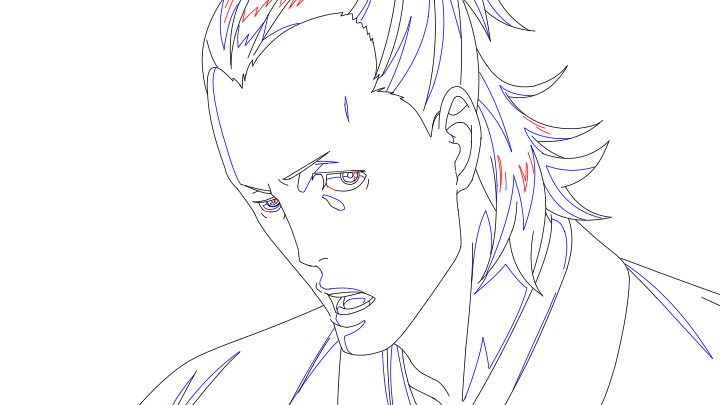
\includegraphics[width=\textwidth]{graphics/douga/49.pdf}
    \caption{Full clean animation frame.}
    \label{fig:segment.ex.full}
\end{subfigure}%
\begin{subfigure}{.5\textwidth}
    \includegraphics[width=\textwidth]{graphics/douga/49_black.pdf}
    \caption{Black segment of the clean animation frame.}
\end{subfigure}
\begin{subfigure}{.5\textwidth}
    \includegraphics[width=\textwidth]{graphics/douga/49_blue.pdf}
    \caption{Blue segment of the clean animation frame.}
\end{subfigure}%
\begin{subfigure}{.5\textwidth}
    \includegraphics[width=\textwidth]{graphics/douga/49_red.pdf}
    \caption{Red segment of the clean animation frame.}
\end{subfigure}%
    \caption{Example of a clean animation frame provided by Tonari Animation segmented by color.}
    \label{fig:segment.ex}
\end{figure}

\subsubsection{Curve Identification}
\label{subsubsec:curve.ident}

In order to indicate to the marked-curve reconstruction model which curve needs to be reconstructed, the second task consists of sampling a pixel lying on a curve not already reconstructed given the input image (more specifically an input image segment, as described in \Cref{subsubsec:colorstroke}) and a canvas image containing already reconstructed curves. In the case of clean line-art images considered in this work, this can simply be done by sampling a random black pixel, where a pixel is considered black if it is closer to 0 than to 1. This pixel is guaranteed to lie on a curve. As an aside, a potential improvement to this algorithm is to always sample the pixel from the largest contiguous area of black pixels, in order to reconstruct the longest curves first. However, this has not been implemented in order to keep the algorithm as simple as possible.

In order to ensure that only curves that have not yet been reconstructed are identified, the canvas image is subtracted from the input image whenever a new curve is added to the canvas and before the marker pixel is sampled. This also helps the marked-curve reconstruction model to not output duplicate curves.

Both the curve identification by sampling black pixels and the subtraction of the canvas image from the input image have the assumption of clean line-art images. Thus, when the line-art vectorization is applied to input images of different domains, these two parts have to be adapted. If there exists a binarization algorithm of considerable quality for this domain (e.g. \citet{DBLP:conf/das/SuLT10}), then simply binarizing images with this algorithm will suffice. Otherwise, one alternative is to train a curve identification model. This alternative would render the entire line-art image vectorization method end-to-end differentiable. The curve identification model would take as input both the input line-art image and the canvas image, where the latter could be appended as a fourth color channel to the former. The output would a vector containing two elements, constrained by the sigmoid function to lie in $[0,1]$, indicating the coordinates of the marker. Then, the architecture would be a convolutional neural network with global average pooling on a filter size of 2 at the end. There are multiple candidates for loss functions. One possibility is to calculate the distance of the marker to all ground truth curves that are not present in the canvas image and taking the minimum. This would require the training images to also be available in vector format.

\subsubsection{Marked-Curve Reconstruction Model Invocation}
\label{subsubsec:model.invok}

In order to vectorize the entire line-art image, the marked-curve reconstruction model has to be invoked iteratively until all curves are reconstructed. This is done in multiple steps, which are laid out in \Cref{alg:iterative.recon}. In this algorithm, the remaining image is the raster image containing curves that are not yet reconstructed. The canvas image is stored as vector image using the \gls{svg} format. It is rasterized when being used to update the remaining curves image.


\begin{algorithm}
  \caption{Iterative Curve Reconstruction.}
  \label{alg:iterative.recon}
  \KwIn{A raster line-art image.}
  \KwOut{A vector line-art image.}
  Segment input image by color\;
  \ForEach{image segment}
  {
  canvas = an empty vector image of the same size as the input image\;
  remaining = image segment\;
  \While{number of black pixels in remaining > $T$;}
  {
  Compute marker by applying curve identification on the remaining image\;
  Centered image = center the remaining image on the marker\;
  reconstructed curve = invoke the marked-curve reconstruction model using the centered image\;
  Inverse the center location of the curve by using the mark location\;
  Add the reconstructed curve to the canvas image\;
  remaining = remaining - rasterized canvas image\;
  }
  Set color of all curves in the canvas image to the segment color\;
  }
  Merge the canvas images\;
  \Return{Merged canvas images}
\end{algorithm}

Note, that Line 5 in \Cref{alg:iterative.recon} constitutes an intuitive stopping criterion enabled by the progressive canvas image subtraction from the remaining image. The curve reconstruction is iteratively applied until the number of black pixels (i.e., the number of possible markers) in the remaining image is greater than some threshold $T$. If the curve identification and reconstruction worked perfectly, the difference between the rasterized canvas image and the remaining image would reach 0 at some point. In this case, the threshold should be set to $T=1$. However, since errors in the reconstructed curves are to be expected, there will remain a number of black pixels that are part of an already reconstructed curve that does not fully cover the curve in the input image. Repeatedly invoking the marked-curve reconstruction model on such pixel artifacts will lead to worse results. Since missing a few curves is not a significant issue, it is tolerable to set the threshold to a low number of black pixels greater than 1. For this algorithm, the threshold is set to $T=\lfloor B*0.1 \rceil$, where $B$ is the number of black pixels in the original image.

\subsubsection{Advantages and Limitations}
\label{subsec:method.limitations}

The theoretical runtime complexity of the algorithm as defined in \Cref{alg:iterative.recon} is in $\mathcal{O}(p)$, where $p$ is the number of black pixels in the input image, which is connected to the number of curves $n$. As the performance of the marked-curve reconstruction model increases, the runtime will be approximately linear in $n$. However, it is possible to significantly reduce the runtime  by processing a batch of curves $b<n$ concurrently, instead of one curve at a time. For this, the curve identification algorithm described in \Cref{subsubsec:curve.ident} can be adapted to sample $b$ black pixels instead of a single black pixel. To decrease the probability of multiple marks belonging to the same curve being sampled, the image should be divided in $b$ patches, with a single mark being sampled in each patch. The marked-curve reconstruction model does not need to be adapted, since it possesses the ability to processes a batch of inputs, which is already done at training time. Note that this adaptation increases the memory requirement by roughly $b$ times. However, since the test dataset is rather small (see \Cref{sec:dataset}), this parallel version of the algorithm has not been implemented.

Furthermore, an advantage of this algorithmic structure is that it significantly eases the effort required to manually fix an output image. While identification of missing curves is a trivial task for humans, fixing wrongly reconstructed curves is tedious. Following this, the algorithm is designed to maximize the former in lieu of the latter. On the one hand, it allows to post-hoc reconstruct curves that were missed by the first run of the algorithm without affecting the rest of the output by simply placing a mark on a random point of the curve in question and invoking the marked-curve reconstruction model. On the other hand, by letting the learned model focus on reconstruction of a single curve, its reconstruction results will be at least better than a model that needs to perform reconstruction and identification of all curves, thereby reducing the need to fix reconstructed curves.

Lastly, there are two issues associated with overlapping curves, i.e., pixels which are part of multiple curves. Firstly, this directly affects the iterative curve reconstruction algorithm. Suppose the marked-curve reconstruction model outputs one of the multiple overlapping curves, then this curve will be placed on the canvas image and removed from the input image. In this process, the overlapping pixels will also be removed, leaving behind a hole in the remaining curves, effectively splitting them. Hence, if the hole is large enough, the curve reconstruction model will reconstruct only one part of the split curve instead of the whole curve. Secondly, the curve reconstruction model will receive ambiguous information on which curve to reconstruct during training in these cases, hampering its ability to derive meaningful gradients at all in the worst case. However, both of these issues are negligible since the amount of overlapping curves is small, as the calculation in \Cref{sec:dataset} shows.


\section{Dataset}
\label{sec:dataset}

The dataset used to train and evaluate the line-art vectorization method consists of two parts: a human-generated and a synthetic dataset. Both datasets contain clean line-art images as vector images using the \gls{svg} file format, with a uniform color for the background (white) and the curves (black). An example indicating the vector primitives used can be seen in \Cref{fig:douga.alternating}, with each primitive represented using a mutually exclusive color. The first part is described in \Cref{subsec:dataset.human} and consists of line-art images drawn by professional and amateur artists. The synthetic part is described in \Cref{subsec:dataset.synthetic}. \Cref{subsec:dataset.limitations} notes irregularities and limitations of the assembled dataset. Steps taken to deal with these irregularities and further processing steps are described in \Cref{subsec:dataset.processing}.

\subsection{Human-generated Dataset}
\label{subsec:dataset.human}
\begin{figure}[h]
    \centering
        \includegraphics[width=\textwidth]{graphics/douga/49-alternating}
    \caption{A clean animation keyframe in vector format with all outline (i.e., black) curves indicated by alternating colors. Original keyframe provided by Tonari Animation.}
    \label{fig:douga.alternating}
\end{figure}

The human-generated data is the most important part of the dataset, since it enables the marked-curve reconstruction model to reconstruct curves in a semantically meaningful way. It consists 20564 vector images from three sources displayed in \Cref{tab:data.subsets}. As noted in \Cref{sec:challenges}, a small dataset of 139 real-world clean animation frames is provided by Tonari Animation, which is detailed in \Cref{subsec:dataset.douga}. While it forms the heart of this dataset, the amount of data is rather limited, necessitating additional sources of data. Two additional sources are used: One of these comes from a sketch cleanup benchmark by \citet{Yan:2020:ABR} and is explained in \Cref{subsec:dataset.sketchbench}. Since this is also rather limited in size, a collection of amateur sketches by \citet{eitz2012hdhso} is used as additional dataset of medium-to-low quality but large quantity.

\begin{table}[]
    \centering
    \begin{tabular}{lrr}
\toprule
 & images & images with overlapping curves \\
\midrule
tonari & 139 & 138 \\
sketchbench & 425 & - \\
tuberlin & 20000 & - \\
\bottomrule
\end{tabular}

    \caption{Summary of the subsets of dataset.}
    \label{tab:data.subsets}
\end{table}

\subsubsection{Tonari Clean Animation Frames}
\label{subsec:dataset.douga}
\Cref{fig:douga.example.clean} shows one of 194 clean animation frames in raster format provided by Tonari Animation for an earlier work by \citet{Kugler-2021}. Since they are not vector images, they cannot be used for this work. However, for 50 of these clean animation frames, the original Clip Studio \citep{clipstudio} files used to draw the images were still available, enabling access to the underlying vector primitives. Additionally, Clip Studio files of 4 sample animation sequences were provided, from which 89 clean animation keyframes and inbetweens could be extracted. An example of this additional data can be seen in \Cref{fig:sample-animation-ex}. In total, this leads to a dataset of 139 clean animation frames in vector format provided by Tonari Animation. Note that inbetweens are very similar to each other (see \Cref{sec:anime.prod}), thus containing a high amount of redundant information, limiting their usefulness to train the model. Still, due to the low amount of available data, all inbetweens are used.

\begin{figure}
    \centering
    \includegraphics[width=\textwidth]{graphics/douga/007AD_DOU_27.pdf}
    \caption{An example of a clean animation frame from a sample animation sequence depicted in \Cref{fig:multiple-douga}, provided by Tonari Animation.}
    \label{fig:sample-animation-ex}
\end{figure}

Since the Clip Studio files provided by Tonari Animation are in a format which cannot be used to train or evaluate the marked-curve reconstruction model, the vector primitives have to be manually extracted from these files. For this, the trial version of Clip Studio version 1.10.5  \citep{clipstudio} was used on a Windows 10 machine. Using the Export Vectors function, each of the 139 clean animation frames was exported as \gls{svg} file. \Cref{fig:clean-frame-vec} shows the result of this extraction on the example in \Cref{fig:douga.example.clean}. The color of the curves is preserved according to the schema defined in \Cref{fig:bg.color-schema}. This information is used by the iterative curve reconstruction algorithm as noted in \Cref{subsubsec:colorstroke}. Note that only curves could be exported, with filled color regions missing from the output. However, as mentioned in \Cref{subsec:cleanframes}, they can trivially be added by bucket filling and are thus not an integral part of the clean animation frame. Hence, only the curves are considered for this work.

It is important to note that while images are available in vector format and can be theoretically displayed at all resolutions, they are generally drawn with a target resolution of 720x405px by Tonari Animation.

\subsubsection{SketchBench}
\label{subsec:dataset.sketchbench}

The rough sketch cleanup benchmark by \citep{Yan:2020:ABR} provides public high-quality line-art vector images. These are sourced from a varied and balanced amount of domains and artists and processed according to a workflow depicted in \Cref{fig:sketchbench.example}. First, 151 sketches of the genres freeform, fashion, products, logos and architecture drawn by various artists are retrieved online. These sketches were drawn on paper or digitally and are only available in raster format. Then, up to 3 out of 7 contracted artists per sketch trace clean vector versions of the rough sketch raster image, yielding 425 \gls{svg} images. These traced vector images contain curves indicating shadows, textures and scaffolds, which are removed to produce clean vector versions of the original rough sketch raster image. Furthermore, the curves are normalized to a constant stroke width.

\begin{figure}[h]
\centering
    \begin{subfigure}{.3\textwidth}
        \includegraphics[width=\textwidth]{graphics/sketchbench/Art_freeform_AG_03.png}
        \caption{A rough sketch drawn on paper as raster image.}
    \end{subfigure}
    \hspace{.01\textwidth}
    \begin{subfigure}{.3\textwidth}
        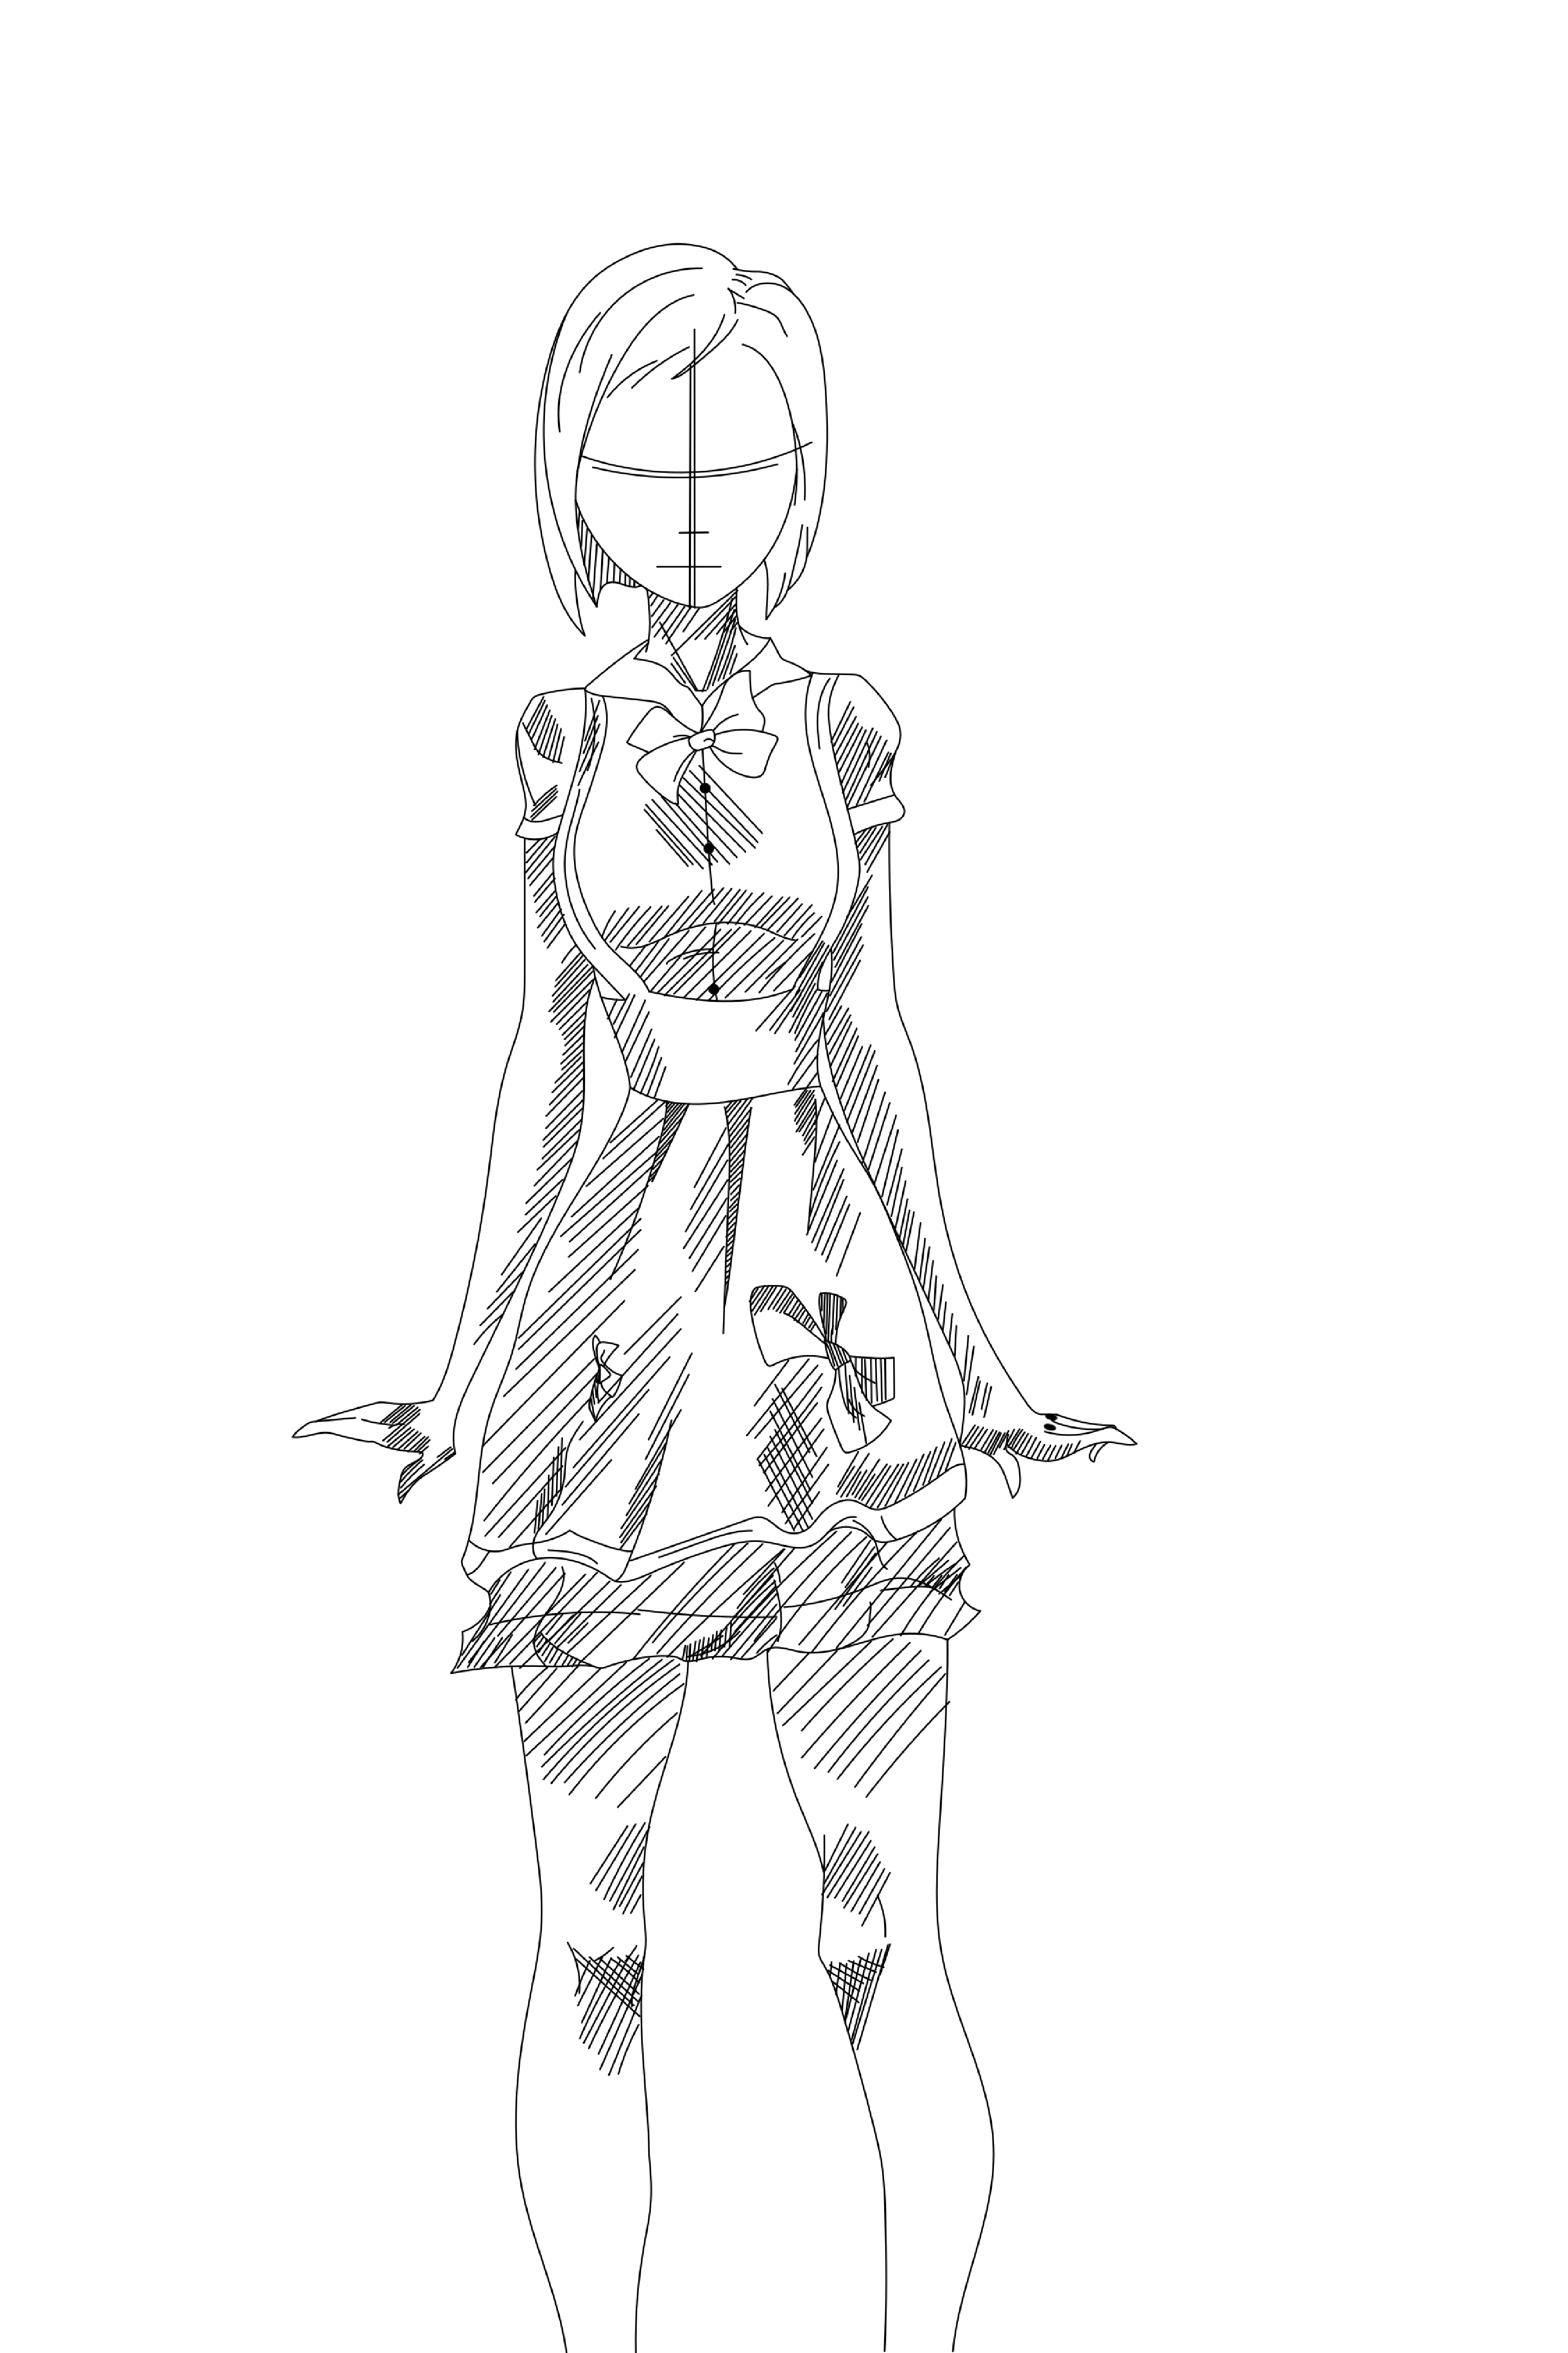
\includegraphics[width=\textwidth]{graphics/sketchbench/Art_freeform_AG_03_Branislav Mirkovic.pdf}
        \caption{Full vector tracing of the original rough sketch.}
    \end{subfigure}
    \hspace{.01\textwidth}
    \begin{subfigure}{.3\textwidth}
        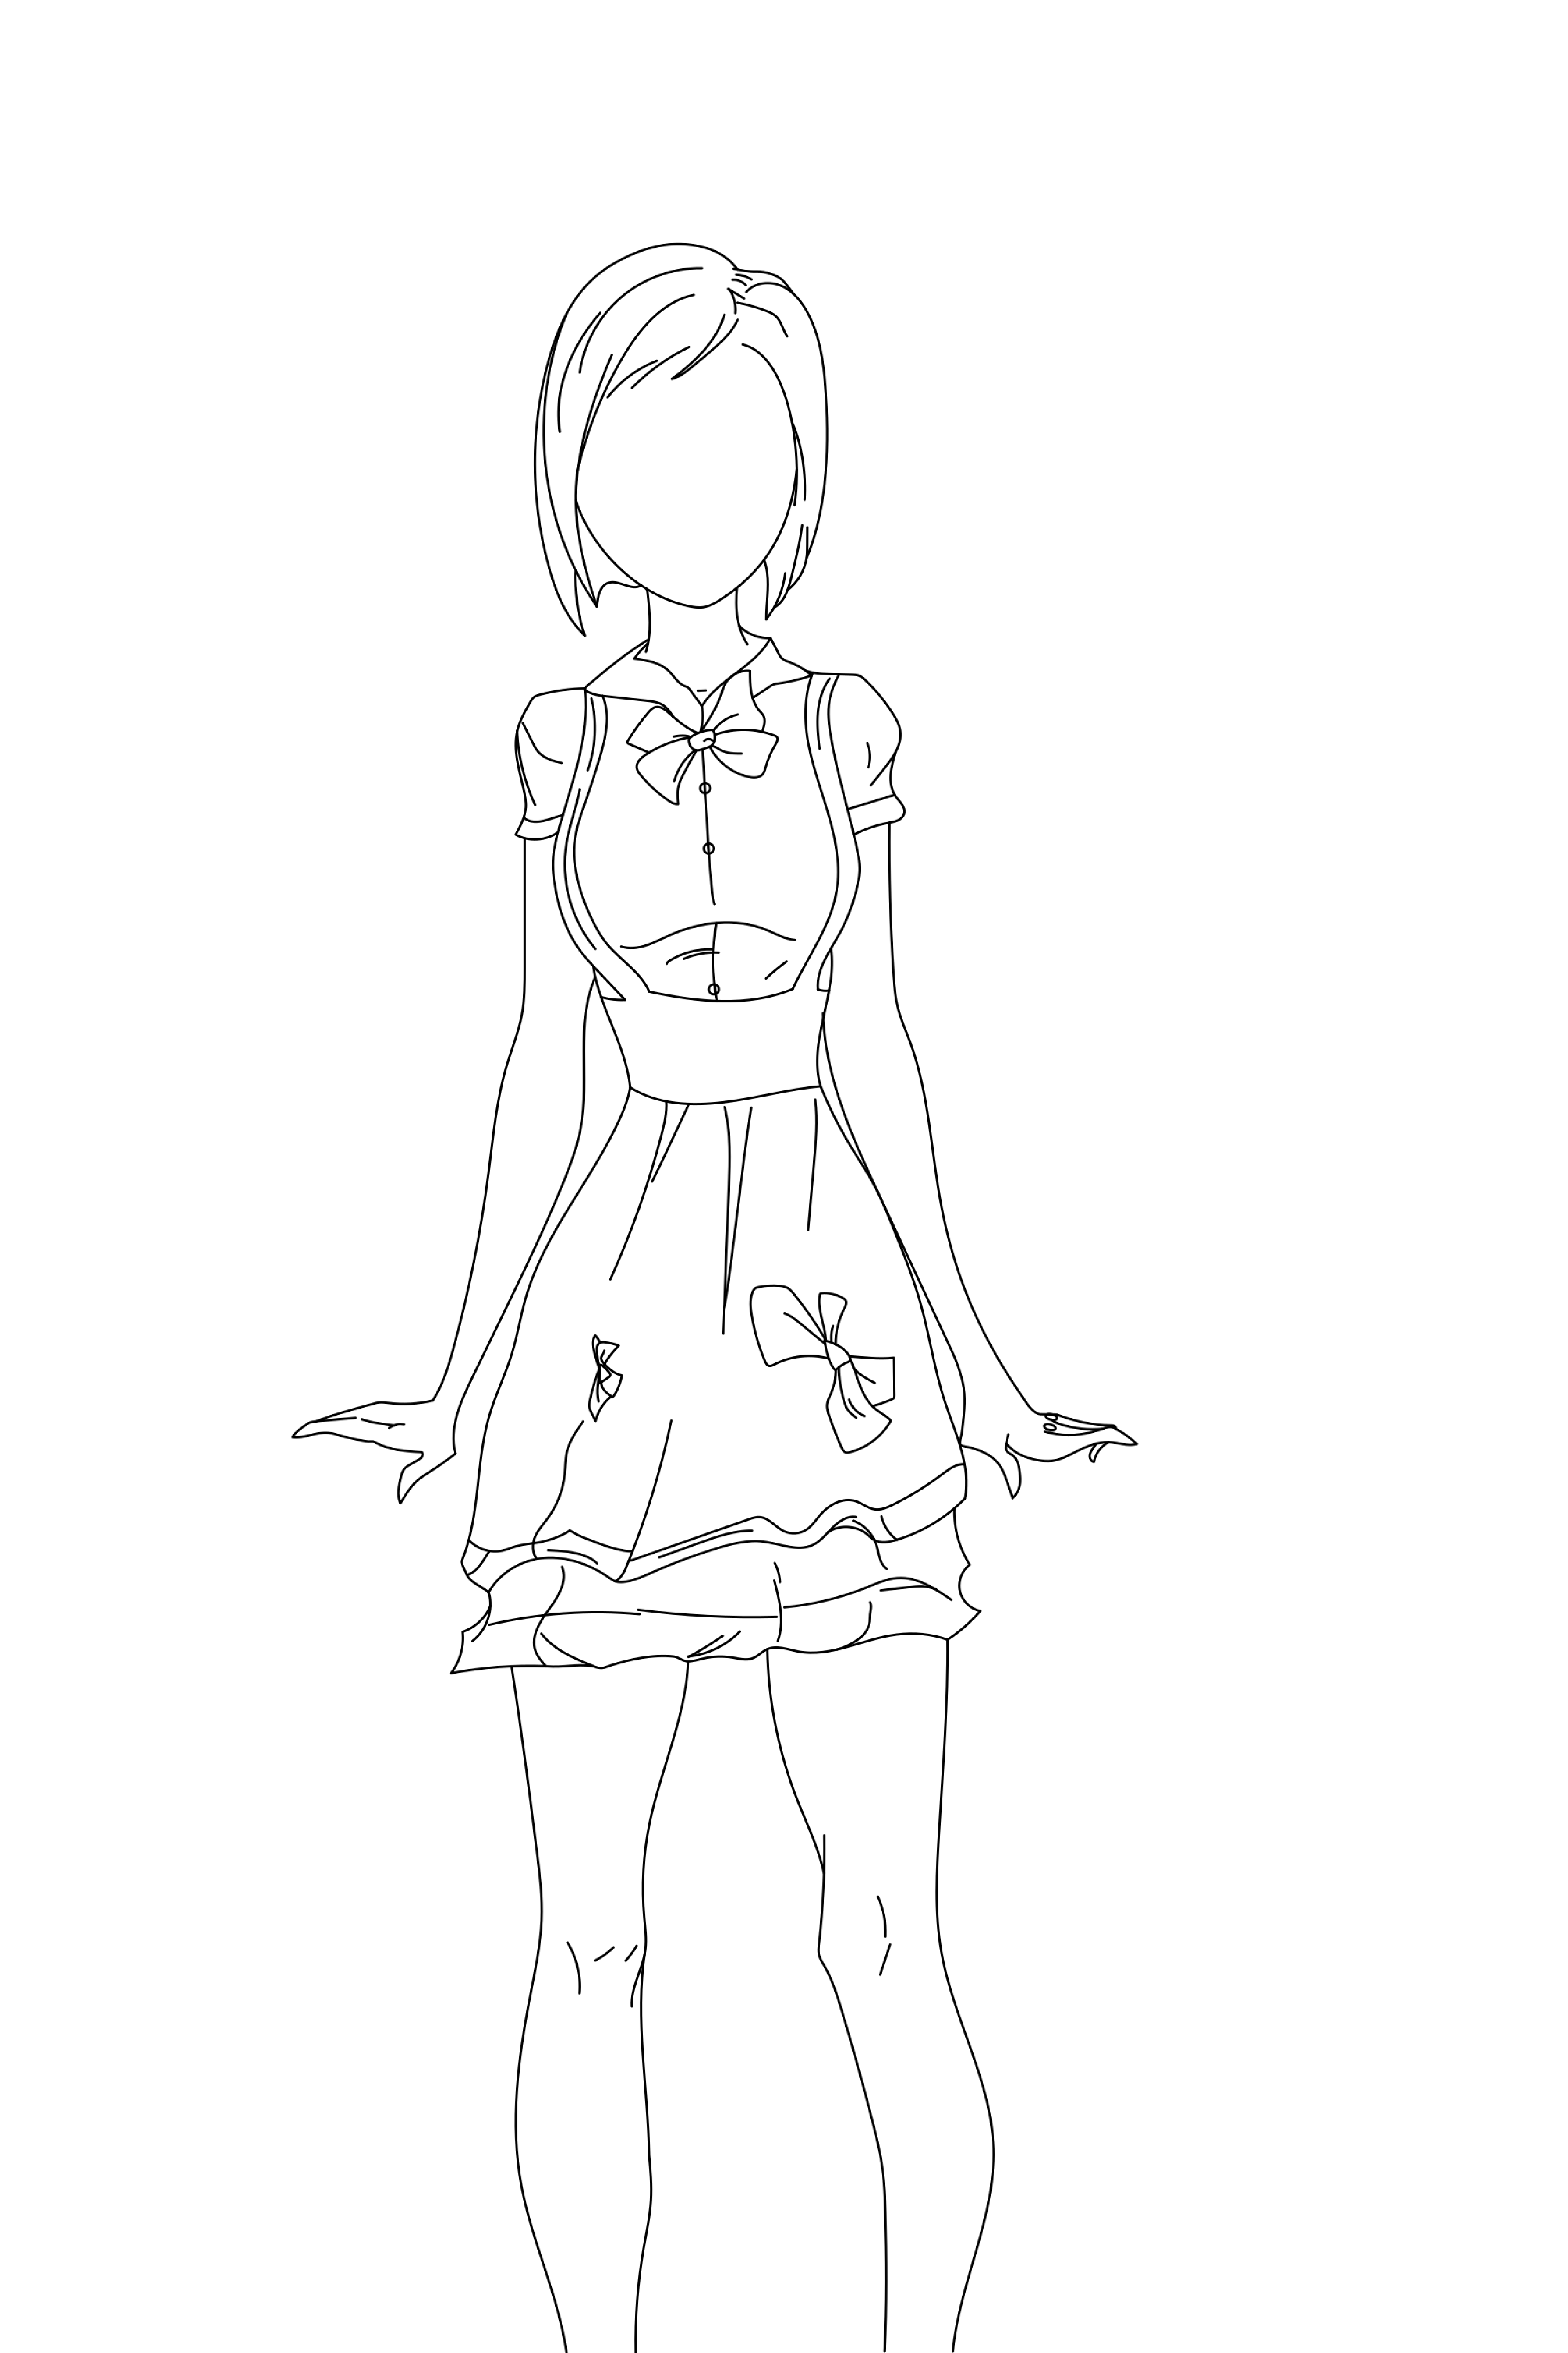
\includegraphics[width=\textwidth]{graphics/sketchbench/Art_freeform_AG_03_Branislav Mirkovic_norm_cleaned.pdf}
        \caption{Normalized and cleaned version of the vector trace.}
    \end{subfigure}
    \caption{Available versions of an example freeform sketch in the SketchBench dataset \citep{Yan:2020:ABR}.}
    \label{fig:sketchbench.example}
\end{figure}

Only clean line-art images are used to train the marked-curve reconstruction model. Hence, the rough raster images and the traces before cleanup are removed, with only the normalized and cleaned versions of the traced sketches remaining in dataset. These images are indicated by the \texttt{norm\_cleaned.svg} suffix of their filename. In total, this leads to a dataset of 425 vector images.

The dataset resembles the Tonari clean animation frames closely, containing only quadratic and cubic bezier curves with a constant stroke width. However, it differs in some respects. Out of the images, sketches of the freeform genre are overrepresented and most closely resemble clean animation frames. However, due to a general lack of data, sketches of all genres are used for this work. Furthermore, there are only black curves in this dataset. Hence, the segmentation noted in \Cref{subsubsec:colorstroke} does not need to be performed on this data.

\subsubsection{TU Berlin amateur sketch collection}

In order to increase the size of the human-generated dataset, the amateur sketch collection by \citet{eitz2012hdhso} is also used. The sketches were collected by TU Berlin for the purpose of creating a classification model. Hence, the dataset contains in total \num{20000} amateur sketches of 250 pre-defined categories. The categories are derived from the LabelMe dataset \citep{DBLP:journals/ijcv/RussellTMF08} and contain objects such as airplanes, houses, and fishes. Examples are displayed in \Cref{fig:tuberlin.example}. The sketches are drawn by \num{1350} amateur artists contracted using Amazon Mechanical Turk. They contain only outlines and are drawn without a reference image, with a median drawing time of 86 seconds. The images are also available in the \gls{svg} format, which can be readily used for this method.

\begin{figure}
    \centering
    \begin{subfigure}{.3\textwidth}
        \includegraphics[width=\textwidth]{graphics/tuberlin/3.pdf}
        \caption{An amateur sketch of the airplane category.}
    \end{subfigure}
    \begin{subfigure}{.3\textwidth}
        \includegraphics[width=\textwidth]{graphics/tuberlin/8801.pdf}
        \caption{An amateur sketch of the house category.}
    \end{subfigure}
    \begin{subfigure}{.3\textwidth}
        \includegraphics[width=\textwidth]{graphics/tuberlin/6561.pdf}
        \caption{An amateur sketch of the fish category.}
    \end{subfigure}
    \caption{Example of the TU Berlin amateur sketch collection by \citet{eitz2012hdhso}.}
    \label{fig:tuberlin.example}
\end{figure}

There exist other collections of amateur sketch vector images such as Quick, Draw! \citep{DBLP:conf/iclr/HaE18}). These could also be added in order to increase the overall dataset size. However, the TU Berlin dataset is already dominating the other, high-quality sources by number of images. If the Quick, Draw! dataset was added, the marked-curve reconstruction model would be even more biased to amateur sketches, to the detriment of performance on professional line art. Hence, other amateur sketch collections are not considered in this work.

\subsubsection{Statistics}
\label{subsec:dataset.stats}

\begin{table}[]
    \centering\begin{tabular}{llrrr}
\toprule
 &  & tonari & sketchbench & tuberlin \\
\midrule
\multirow[t]{2}{*}{paths} & median & 495.00 & 44.00 & 13.00 \\
 & \acrshort{iqr} & 210.00 & 96.00 & 15.00 \\
\cline{1-5}
\multirow[t]{2}{*}{curves} & median & 1476.00 & 156.00 & 78.00 \\
 & \acrshort{iqr} & 1041.00 & 381.00 & 72.00 \\
\cline{1-5}
\multirow[t]{2}{*}{curves / path} & median & 1.00 & 2.00 & 4.00 \\
 & \acrshort{iqr} & 2.00 & 1.00 & 4.00 \\
\cline{1-5}
\multirow[t]{2}{*}{path length} & median & 65.61 & 219.82 & 176.01 \\
 & \acrshort{iqr} & 29.90 & 327.81 & 223.20 \\
\cline{1-5}
\multirow[t]{2}{*}{curve length} & median & 9.60 & 67.82 & 32.17 \\
 & \acrshort{iqr} & 6.83 & 106.37 & 19.42 \\
\cline{1-5}
\multirow[t]{2}{*}{overlap curves} & median & 10.00 & - & - \\
 & \acrshort{iqr} & 10.00 & - & - \\
\cline{1-5}
\bottomrule
\end{tabular}

    %{\tiny \begin{tabular}{llrrr}
\toprule
 &  & tonari & sketchbench & tuberlin \\
\midrule
\multirow[t]{2}{*}{paths} & median & 495.00 & 44.00 & 13.00 \\
 & \acrshort{iqr} & 210.00 & 96.00 & 15.00 \\
\cline{1-5}
\multirow[t]{2}{*}{curves} & median & 1476.00 & 156.00 & 78.00 \\
 & \acrshort{iqr} & 1041.00 & 381.00 & 72.00 \\
\cline{1-5}
\multirow[t]{2}{*}{curves / path} & median & 1.00 & 2.00 & 4.00 \\
 & \acrshort{iqr} & 2.00 & 1.00 & 4.00 \\
\cline{1-5}
\multirow[t]{2}{*}{path length} & median & 65.61 & 219.82 & 176.01 \\
 & \acrshort{iqr} & 29.90 & 327.81 & 223.20 \\
\cline{1-5}
\multirow[t]{2}{*}{curve length} & median & 9.60 & 67.82 & 32.17 \\
 & \acrshort{iqr} & 6.83 & 106.37 & 19.42 \\
\cline{1-5}
\multirow[t]{2}{*}{overlap curves} & median & 10.00 & - & - \\
 & \acrshort{iqr} & 10.00 & - & - \\
\cline{1-5}
\bottomrule
\end{tabular}
}
    \caption{Summary statistics for the human-generated subsets of the dataset}
    \label{tab:dataset.statistics}
\end{table}

All images in the human-generated dataset are clean line-art images in vector format. The images contain a uniform background and cubic bezier curves, which are grouped together to form \textit{paths}. \Cref{tab:dataset.statistics} shows statistics of the dataset and its subsets. Note that the median is used as robust location estimate and \gls{iqr} as robust scale estimate. This is due to the assumption that there are outliers in the data, which can have an outsized influence due to the limited size (excluding the TU Berlin subset). \Cref{fig:stats-49} shows the left skewed nature of distributions of the example clean animation frame depicted in \Cref{fig:segment.ex.full} and corroborates this assumption.

\begin{figure}
    \centering
    \begin{subfigure}{.5\textwidth}
    \centering
    \includegraphics[width=\textwidth]{graphics/data_stats/path_len.pdf}
    \caption{Histogram of the length of each path.}
    \label{fig:path_len}
\end{subfigure}%
    \begin{subfigure}{.5\textwidth}
    \centering
    \includegraphics[width=\textwidth]{graphics/data_stats/curve_len.pdf}
    \caption{Histogram of the length of each curve.}
    \label{fig:curve_len}
\end{subfigure}
    \begin{subfigure}{.5\textwidth}
    \centering
    \includegraphics[width=\textwidth]{graphics/data_stats/no_curve_per_path.pdf}
    \caption{Histogram of the number of curves per path.}
    \label{fig:no_curve_per_path}
\end{subfigure}
    \caption{Statistics of the clean animation frame depicted in \Cref{fig:segment.ex.full}.}
    \label{fig:stats-49}
\end{figure}

The statistics displayed in \Cref{tab:dataset.statistics} help with deciding on which level of graphic primitives the method should be based. There are two options: basing the method on \textit{curves}, which gives more flexible and fine control over the vector output and reduces the complexity for the model by only requiring to reconstruct a single primitive, or \textit{paths}, which can be considered more semantically meaningful but would require the model to reconstruct a group of curves at a time. 

\Cref{tab:dataset.statistics}  shows that the average number of curves per path for the high-quality subsets is very small. To exemplify this, \Cref{fig:no_curve_per_path} shows the distribution of the number of curves per path in the image depicted in \Cref{fig:segment.ex.full}. There seems to be a bimodal distribution, with most paths either consisting of a single curve or more than 2 curves. It is clear that the overwhelming majority of paths belongs to the former, making this higher-level primitive somewhat redundant. Interestingly, both the average and the variance of the number of curves per path in the TU Berlin subset is significantly higher than in the high-quality subsets, indicating that a significant amount of amateur artists made more use of this primitive than professional artists. However, since the focus of the method should lie on the high-quality subsets, it is decided to base the method on curves and to discard path information.

Another important information for the decision between curves and paths is the average length of each, which is measured in pixels. Interestingly, \Cref{tab:dataset.statistics} shows that the average curve length of Tonari clean animation frames is significantly lower than the other two subsets, with SketchBench images having the longest curves on average. The same finding is maintained for the average path length. Furthermore, the ratio of curve length by path length is similar for the Tonari and TU Berlin subsets, with the SketchBench subset having roughly double the ratio. In general, and even for the Tonari clean animation frames, curves seem on average to be long enough to be independently recognized and restored, further corroborating the use of curves as graphical primitive. Still, due to the high variance of curve and path lengths and the seemingly bimodal distribution of the amount of curves per path, using paths as base graphical primitive is also a legitimate avenue.

Furthermore, when looking at the statistics, two peculiarities in the data become apparent. Firstly, \Cref{tab:dataset.statistics,tab:data.subsets} show that there exists a significant amount of overlapping curves, where two curves are considered overlapping if they have more than one intersection and there is at least one intersection that is not at the start or the end point, with a tolerance of $0.1$. This calculation is computationally expensive, as this requires comparing every curve with every other curve. Hence, this information is only provided for the important Tonari subset. Interestingly, the average number of overlapping curves per image is $36\pm36$ with the average number of overall curves per image being $1476\pm1041$. This suggests that most images contain only a little amount of overlapping curves. However, since nearly all images have at least one curve overlapping another, this needs to be accounted for when dealing with these images.

\subsection{Synthetic Dataset}
\label{subsec:dataset.synthetic}
Since the human-generated part of the dataset is limited in size, the dataset also includes synthetic data. While automatic vectorization of existing clean line-art raster images is not yet possible (as this is the whole purpose of this work), the reverse, i.e., the rasterization of vector line-art images is trivial, as described in \Cref{sec:vec}. Hence, for the synthetic data, line-art vector images are automatically generated and rasterized. However, automatic generation of line-art vector images is challenging. Since automatically generating high-quality line-art vector images such as the Tonari clean animation frames is still an open research question, one has to resign oneself to a lower quality of the generated images. Due to this low quality, the synthetic dataset is combined with the human-generated dataset at a 1 to 5 ratio at train time, i.e., for every training epoch, the human-generated vector images are topped up with synthetic vector images matching a fifth of their amount.

The generation algorithm defined for this work simply produces a low number of random cubic bezier curves for a vector image. The main hyperparameter of the algorithm is the curve amount range, which is set to $[3,8]$ unless otherwise stated. This means that the algorithm produces at least 3 and at most 8 curves per image, with the actual number being chosen randomly. The generation is restricted to this low amount in order to minimize the probability of overlapping curves, which otherwise would need to be detected and removed in a computationally costly manner. The curves themselves are generated by sampling 8 random numbers independently from the uniform distribution with interval $[0,1)$. These numbers constitute the coordinates of the 4 points needed to parameterize a cubic bezier curve. Since the synthetic image needs to have the same size as the human-generated images, the x-coordinates and y-coordinates of the random points are scaled by the image width and image height chosen by the human-generated dataset, respectively.

\begin{figure}
\centering
    \begin{subfigure}{.45\textwidth}
        \includegraphics[width=\textwidth]{graphics/synth-3.pdf}
        \caption{Image with 3 random cubic bezier curves.}
    \end{subfigure}
    \begin{subfigure}{.45\textwidth}
        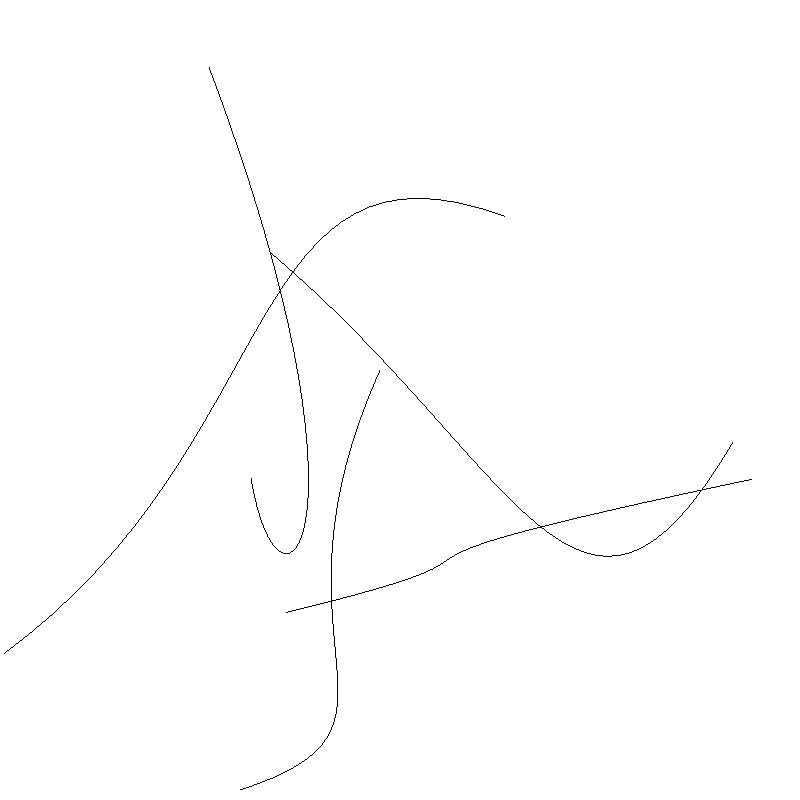
\includegraphics[width=\textwidth]{graphics/synth-5.pdf}
        \caption{Image with 5 random cubic bezier curves.}
    \end{subfigure}
    \caption{Example images of the synthetic dataset. Note the apparent low quality in comparison with other example images in \Cref{fig:sample-animation-ex,fig:sketchbench.example,fig:tuberlin.example}.}
    \label{fig:synthetic-example}
\end{figure}

\Cref{fig:synthetic-example} shows examples of synthetic line-art images. It can be seen that they differ in quality from the human-generated dataset. Furthermore, they contain significantly fewer curves. In combination, the curves in the human-generated dataset form recognizable objects, while the random synthetic curves do not represent shapes that can be found in clean animation frames. Hence, it is clear that the synthetic dataset is not similar to the clean animation frames (on which the method is intended to be used on) and is wholly insufficient to train the marked-curve reconstruction model. However, by being used in combination with the human-generated dataset, it can serve another purpose: it provides new learning signals to the model. Importantly, the human-generated dataset contains a limited amount of semantic objects to the visual presence of which the model could theoretically overfit. On the other hand, the synthetic images contain only curves that are \textit{guaranteed} to not be in a semantic relationship with each other. Therefore, the synthetic dataset forces the model to focus on reconstructing a single curve correctly when no semantic visual indications are present. Furthermore, the synthetic data likely contains curve shapes not present in the human-generated data. Fitting the model to this data can be useful when the model is applied to images containing objects and curves that are visually very different from the ones in the human-generated dataset. Keep in mind, however, that this is only beneficial to the model if the semantics-free data forms but a small part of the entire dataset.

To optimize the runtime of the algorithm, a batch of points is directly created on the \gls{gpu} per invocation. The images are synthesized on-line instead of precomputed, i.e., the generation algorithm is run concurrently to the training process, generating new data for each training iteration. Another possibility is to run the generation algorithm beforehand and to save a large amount of precomputed random images on disk. These could then be loaded at training time. The on-line variant is chosen because it has three advantages: firstly, it ensures that every batch generated consists of new data, preventing overfitting if the model is run for a long time. Secondly, it requires no disk space, while the disk space required for the precomputed images can be considerably large. Thirdly, it makes changes to the generation algorithm easier, since the images do not have to be precomputed after every change. Furthermore, the runtime difference between generating a batch of 8 random numbers directly on the \gls{gpu} versus loading the images from disk to the \gls{gpu} is negligible.

\subsection{Limitations}
\label{subsec:dataset.limitations}
The dataset assembled for this work is of considerable quality, but still comes with a range of limitations. It is important to note that these significantly affect the model training and the evaluation.

Since publicly available clean animation frames in vector format are rather limited, the amount of high-quality data in the dataset is considerably small. This is a major limitation of the dataset, as training a deep learning model usually requires a large amount of data. While the synthetic data introduced in \Cref{subsec:dataset.synthetic} increases the dataset size significantly, it is not of sufficient quality to effectively alleviate this limitation. There exist some other publicly available high-quality data, such as sample data of open animation tools like OpenToonz \citep{opentoonz}. However, the amount of vector images in these samples is very limited. Additional sample data exists for proprietary animation tools like CACANi \citep{cacani}, which can not be used without the tool and are similarly few in number. Another possibility is to extend the dataset with sources from different domains such as product design sketches \citep{OpenSketch19}. This was not considered in this work beyond the SketchBench subset due to the focus on clean animation frames.

Another limitation stems from the assumption that different artists draw vector images using slightly different graphical primitives and topologies. Hence, the distribution of artists in this dataset affects the performance of the line-art vectorization method. This distribution is rather skewed in the Tonari subset. Out of this subset, the initial 50 images were drawn by a single artist, while the artist information about the 89 keyframes and inbetweens is unknown. On the other hand, the distribution of artists in the SketchBench and TU Berlin subsets are rather even, which renders them helpful in preventing possible overfit to the artist distribution in the Tonari subset.

\subsubsection{Irregularities}
\label{subsec:dataset.limitations.irregularities}

Furthermore, there are various irregularities in the Tonari clean animation frames that need to be accounted for when processing them. The biggest is that there are a number of apparently incorrectly drawn curves in the images. These are ostensibly erased by drawing a white curve with high stroke width over them. \Cref{fig:white-patch} shows an example of such a patch, which is not visible when rasterized, but is still present in the underlying vector topology. Another irregularity is that curves often extend outside the viewbox, as depicted in \Cref{fig:50_extended_height}.

\begin{figure}
    \centering
    \begin{subfigure}{\textwidth}
    \centering
        \includegraphics[width=\textwidth,trim={13em 15em 32em 12em},clip]{graphics/douga/39.pdf}
        \caption{The vector image rasterized normally, zoomed into the right upper eye region.}
    \end{subfigure}
    \begin{subfigure}{\textwidth}
        \includegraphics[width=\textwidth,trim={13em 15em 32em 12em},clip]{graphics/douga/39_magenta_patch.pdf}
        \caption{The vector image rasterized normally with the color of the white patch set to magenta, thus making it visible.}
    \end{subfigure}
    \begin{subfigure}{\textwidth}
        \includegraphics[width=\textwidth,trim={13em 15em 32em 12em},clip]{graphics/douga/39_patch_removed.pdf}
        \caption{The vector image rasterized with the white patch removed, rendering the underlying incorrect curve visible.}
    \end{subfigure}
    \caption{An example of a white patch being used to correct incorrect curves. While the patch and the incorrect curve is not visible in the rasterized image, it is still present in the vector structure of the image. The full clean animation frame can be seen in \Cref{fig:douga.example.clean,fig:clean-frame-vec}.}
    \label{fig:white-patch}
\end{figure}

\begin{figure}
    \centering
    \begin{subfigure}[t]{.45\textwidth}
    \caption{The vector image rasterized using the specified view box.}
    \includegraphics[width=\textwidth]{graphics/douga/50.pdf}
    \end{subfigure}
    \begin{subfigure}[t]{.45\textwidth}
    \caption{The vector image rasterized using a view box of 720x465px.}
    \includegraphics[width=\textwidth]{graphics/douga/50_extended_height.pdf}
    \end{subfigure}
    \caption{An example of a clean animation frame with curves extending outside of the specified view box of 720x405px. Notice the extended curves at the bottom. Original clean animation frame provided by Tonari Animation.}
    \label{fig:50_extended_height}
\end{figure}

Additionally, some images contain a significant amount of overlapping curves, as noted in \Cref{tab:dataset.statistics}. \Cref{tab:data.subsets,tab:dataset.statistics} show that Tonari clean animation frames contain $39\pm39$ overlapping curves on average, with almost all images containing overlapping curves. As an example, the image shown in \Cref{fig:sample-animation-ex} contains 428 overlapping curves. This includes both curves with a long overlap, as displayed in \Cref{fig:overlapping.long} and curves with a minor overlap, as displayed in \Cref{fig:overlapping.short}. As noted in \Cref{subsec:method.limitations}, overlapping curves can lead to incorrect outputs of the line-art vectorization method.

\begin{figure}
\centering
    \begin{subfigure}{.45\textwidth}
    \includegraphics[width=\textwidth,trim={34em 24em 27em 24em},clip]{graphics/douga/007AD_DOU_27.pdf}
        \caption{The frame depicted in \Cref{fig:sample-animation-ex} zoomed in to the cap region showing a black and a blue curve in the middle with a long overlap.}
        \label{fig:overlapping.long}
    \end{subfigure}
    \begin{subfigure}{.45\textwidth}
    \includegraphics[width=\textwidth,trim={38em 20em 25em 29em},clip]{graphics/douga/007AD_DOU_27.pdf}
        \caption{The frame depicted in \Cref{fig:sample-animation-ex} zoomed in to the right eye, showing two black curves on the left of the eye with a minor overlap.}
        \label{fig:overlapping.short}
    \end{subfigure}
    \caption{Examples of overlapping curves in the clean animation frame displayed in \Cref{fig:sample-animation-ex}.}
    \label{fig:overlapping}
\end{figure}

Altogether, these irregularities are not apparent once the vector images are rasterized, but are still problematic when the vector structure of the images is used for training and evaluating the method.

\begin{table}[]
    \centering
    \definecolor{000000}{HTML}{000000}
\definecolor{0000ff}{HTML}{0000ff}
\definecolor{ffffff}{HTML}{ffffff}
\definecolor{ff0000}{HTML}{ff0000}
\definecolor{00ff00}{HTML}{00ff00}
\definecolor{120a0a}{HTML}{120a0a}
\definecolor{0c0606}{HTML}{0c0606}
\definecolor{180d0d}{HTML}{180d0d}
\definecolor{ff8000}{HTML}{ff8000}
\definecolor{49ff49}{HTML}{49ff49}
\begin{tabular}{llrr}
\toprule
hex string & Color & Part of schema & Number of paths \\
\midrule
\#000000 & \cellcolor{000000}\color{000000}000000 & True & 45289 \\
\#0000ff & \cellcolor{0000ff}\color{0000ff}0000ff & True & 13944 \\
\#ffffff & \cellcolor{ffffff}\color{ffffff}ffffff & False & 5149 \\
\#ff0000 & \cellcolor{ff0000}\color{ff0000}ff0000 & True & 3728 \\
\#00ff00 & \cellcolor{00ff00}\color{00ff00}00ff00 & True & 486 \\
\#120a0a & \cellcolor{120a0a}\color{120a0a}120a0a & False & 76 \\
\#0c0606 & \cellcolor{0c0606}\color{0c0606}0c0606 & False & 63 \\
\#180d0d & \cellcolor{180d0d}\color{180d0d}180d0d & False & 10 \\
\#ff8000 & \cellcolor{ff8000}\color{ff8000}ff8000 & False & 7 \\
\#49ff49 & \cellcolor{49ff49}\color{49ff49}49ff49 & False & 6 \\
\bottomrule
\end{tabular}

    \caption{The colors used in the Tonari clean animation frames. Colors not part of the clean animation frame schema defined in \Cref{fig:bg.color-schema} are indicated.}
    \label{tab:stroke_color_counter}
\end{table}

There are also two irregularities that are visible both in vector and in raster format. One of them can be seen when considering the color distribution of paths shown in \Cref{tab:stroke_color_counter}. As only the Tonari clean animation frames contain colors other than black, \Cref{tab:stroke_color_counter} only shows information about this subset. It can be seen that there is a considerable amount of paths of a different color than the ones allowed according the the schema defined in \Cref{fig:bg.color-schema}. White is the most present color that is not in the schema, which can be explained with the white patches displayed in \Cref{fig:white-patch}. The other colors not allowed by the schema are only used by less than 200 paths. It can safely be assumed that these are artifacts of artists choosing a slightly wrong color while drawing.

\begin{figure}
    \includegraphics[width=\textwidth]{graphics/data_stats/stroke_width_counter.pdf}
    \caption{Number of curves per stroke width other than 2px in the Tonari clean animation frames.}
    \label{fig:diff.stroke.width}
\end{figure}

\begin{figure}
    \centering
    \begin{subfigure}{.45\textwidth}
        \includegraphics[width=\textwidth]{graphics/douga/007AD_DOU_3.pdf}
        \caption{The clean animation frame with the irregular patch.}
    \end{subfigure}
    \begin{subfigure}{.45\textwidth}
        \includegraphics[width=\textwidth]{graphics/douga/007AD_DOU_3_nopatch.pdf}
        \caption{The clean animation frame with the irregular patch removed.}
    \end{subfigure}
    \caption{An example of an irregular patch in an animation sequence frame provided by Tonari animation.}
    \label{fig:patch.example}
\end{figure}

The other irregularity is the existence paths with a stroke width that differs from the constant stroke width defined for the image. These are present in some Tonari clean animation frames. Keeping in mind that the constant stroke width for clean animation frames is set to 2px, the distribution of paths with a different stroke width is displayed in \Cref{fig:diff.stroke.width}. They are mostly either white patches as described in \Cref{subsec:dataset.limitations,fig:white-patch} or spurious indications and corrections in the sample animation sequence frames displayed in \Cref{fig:patch.example}.

While it might seem trivial to manually fix the irregularities mentioned in this section at a first glance, it turns out to be impossible for non-professional artists. Instead, automatic preprocessing steps are taken to reduce the amount of irregular curves, which are described in \Cref{subsec:dataset.processing}. However, note that the preprocessing steps are rudimentary and conservative, and do not exhaustively remove all irregular curves. This is especially the case for the types of overlapping curves depicted in \Cref{fig:overlapping}, where it is impossible to unambiguously remove one of the overlapping curves.

\subsection{Processing}
\label{subsec:dataset.processing}

The dataset described in this section consists of human-generated and synthetic vector images, where the former are stored on disk in the \gls{svg} format. Before these human-generated images can be used to train or evaluate the method, several preprocessing steps have to be applied, which are described below. The images are processed in parallel using GNU parallel 20220922 \citep{tange_ole_2022_7105792}, with the processing steps implemented using Python 3.8.12 \citep{python}.

\subsubsection{Curve correction}
The first preprocessing steps are motivated by the statistics and irregularities mentioned in \Cref{tab:dataset.statistics,subsec:dataset.limitations}. Since the line-art vectorization method is based on curves instead of paths as graphical primitive, the vector images are converted into flat images only consisting of curves. In order words, paths and other group structures are removed from the vector files using  Inkscape 1.0 \citep{Inkscape}.

The next preprocessing step is to remove irregular curves from the Tonari subset. These include curves with a color that is not allowed by the clean animation frame schema defined in \Cref{fig:bg.color-schema} and curves with a stroke width that is different from the constant stroke width defined for the clean animation frames (i.e., 2px). As already established in \Cref{tab:stroke_color_counter}, the incorrectly colored curves are few in number, thus making them safe to remove. The curves with irregular stroke width are larger in number, but are not part of the semantic structure of the clean animation frame. Recall that they mostly include white patch corrections or other indications as shown in \Cref{fig:white-patch,fig:patch.example}. Hence, it is safe to remove these curves.

While it might seem visually counter-intuitive to remove white patches, as this renders visible curves which the artist intended to hide, it makes sense when considering the underlying vector structure. Drawing white patches over curves only alters their appearance once rasterized, but does not affect their vector representation. Furthermore, these white patches are often drawn over only a part of a curve. Hence, it is challenging to unambiguously derive the correct vector representation of only the curves (or, only the parts of curves) which are intended to be shown. Therefore, white patches are simply removed entirely to lay bare all curves and ensure equivalence between the raster and vector representation of the image. A more conservative alternative would be to sidestep the ambiguity and simply remove all curves which intersect with a white patch. This alternative was not considered in this work as this would greatly reduce the already scarce amount of training data.

Note that, as white patches make up a large portion of overlapping curves, removing them also reduces this issue. However, there still remain overlapping curves of the type depicted in \Cref{fig:overlapping}, which cannot be easily removed automatically.

For this preprocessing step, the svgelements 1.9.5 \cite{svgelements} Python package is used.

\subsubsection{Rasterization}

It is important that all images in the dataset are available in vector format, which enables them to be used to compute the loss for the model and to evaluate vectorization methods. Furthermore, raster versions of these images are required as input data for the vectorization methods. All subsets in the dataset provide raster image versions of the vector images. However, in order to ensure consistency across the input images, the same rasterization scheme is applied to all.

For the consistent rasterization, one option would be to use the rasterization algorithm used by Clip Studio \citep{clipstudio} for all images, since this would perfectly match the clean animation frame images in production at Tonari Animation. However, this was not done for two reasons: firstly, the rasterization algorithm used in Clip Studio could not be determined and cannot easily be used programmatically. Secondly, using a different rasterization algorithm shows that the model does not overfit to a specific rasterization algorithm. Hence, the open source CairoSVG 2.5.2 \citep{cairosvg} algorithm was used for the rasterization. It was applied to all curves of all vector images with consistent settings consisting of a uniform curve color, no fill color and round line endings. The raster images are stored using the \gls{png} format. Furthermore, note that these raster images are not just important as input data, but also to compute the raster-based loss mentioned in \Cref{subsubsec:model.training}. The loss is computed using rasterized input images and the model output rasterized using the differentiable rasterizer by \citet{Li:2020:DVG}. Since the differentiable rasterizer is already used for the model outputs, it would be possible to use the same rasterizer for the inputs as well. However, CairoSVG \citep{cairosvg} is preferred for this purpose due to its significantly lower runtime. Moreover, \Cref{fig:rasterization.comparision} shows that the rasterization output of CairoSVG \citep{cairosvg} is visually similar enough to the differentiable rasterizer \citep{Li:2020:DVG}.

\begin{figure}
    \centering
    \begin{subfigure}{.45\textwidth}
        \includegraphics[width=\textwidth]{graphics/sketchbench/raster/Art_freeform_AG_03_Branislav Mirkovic_norm_cleaned_cairosvg.png}
        \caption{Rasterization using CairoSVG \citep{cairosvg}.}
    \end{subfigure}
    \begin{subfigure}{.45\textwidth}
        \includegraphics[width=\textwidth]{graphics/sketchbench/raster/Art_freeform_AG_03_Branislav Mirkovic_norm_cleaned_diffvg.png}
        \caption{Rasterization using the differentiable rasterizer by \citet{Li:2020:DVG}.}
    \end{subfigure}
    \caption{The example vector image of \Cref{fig:sketchbench.example} rasterized using the differentiable rasterizer by \citet{Li:2020:DVG} and CairoSVG \cite{cairosvg} with the same settings. Note that, even though the former is a differentiable rasterizer, the results are visually similar, save for slightly thicker strokes.}
    \label{fig:rasterization.comparision}
\end{figure}

An important decision of the rasterization algorithm is the resolution. While vector images can be displayed at any resolution, the resolution of the raster images significantly affects the output quality. Since the Tonari clean animation frames were drawn for a 720x405px resolution, it can be assumed that real-world clean animation frames on which the vectorization method needs to be applied will be available at a similar resolution. Hence, the resolution of the rasterization resolution is chosen as the highest exponential of 2 smaller than the width of 720px, i.e., 512x288px. Choosing a resolution that is lower than the target resolution both helps with preventing overfitting to the clean animation frame resolution and trains the model to perform well at lower resolutions. Note that the image is squared to show that the model does not overfit to the aspect ratio of clean animation frames. All vector images in the dataset are rasterized consistently to 512x288px, preserving the aspect ratio with the larger of the width or height set to 512.

Another important decision during rasterization is the stroke width, which is usually set using pixel values and therefore visually connected to the resolution. Due to the homogeneous nature of the stroke width of the processed curves, it can be freely set to a consistent value for all vector images. The stroke width is rather arbitrarily set to 0.512px for all images. This value is a bit lower than the stroke width used for the Tonari clean animation frames, which is 2px for a resolution of 720x405px. This ensures that the method does not overfit to the clean animation frame stroke width. Still, this stroke width in combination with the resolution is large enough that the marked-curve reconstruction model could in theory notice all curves.

The raster images are represented using the \gls{rgb} color model, i.e., using 3 color channels with interval $[0,255]$. As described in \Cref{subsec:io}, the channels are scaled by 255 to produce channels with interval $[0,1]$. Since all raster images are monochrome (even the Tonari clean animation frames after the segmentation by color mentioned in \Cref{subsubsec:colorstroke}), it is also possible to use a single channel instead. However, as noted in \Cref{subsec:io}, both variants perform similarly, with the \gls{rgb} variant allowing easier generalization to different domains and model architectures.

\subsubsection{Data Augmentation}
\label{subsec:dataaug}

After the preprocessing steps, data augmentation is performed on the human-generated dataset. Data augmentation is another technique to synthetically increase the dataset size and consists of applying meaningful transforms to existing data to derive new data. An additional benefit of data augmentation is that it forces the model to be equivariant to these transformations. Usual image processing data augmentation techniques are based on raster images and cannot be used for this work, since the augmented raster image needs to correspond to the original vector image. Hence, data augmentation techniques are derived for and applied on vector images. The resulting new images are then rasterized to produce corresponding transformed vector and raster images. Similar to the synthetic dataset explained in \Cref{subsec:dataset.synthetic}, the data augmentation is performed on-line, i.e., concurrently to the training process.

The data augmentation transformations are efficiently implemented as curve manipulations using the svgpathtools 1.4.4 package \citep{svgpathtools}. They include curve mirroring, rotation, reversion and dropout. All transformations are independently applied with a probability of 50\% per iteration. The transformations are displayed in \Cref{fig:dataaug} and explained in the following: Curve reversion reverses the orientation of the curves, i.e., swaps the order of the curve parameters, which affects only the vector structure and not the visual representation. While curve mirroring flips curves according to the horizontal axis of the image, curve rotation flips curves according to the diagonal of the image. These augmentations make the model more robust to different curve orientations. On the other hand, curve dropout removes a random percentage of curves lying between $[0\%,90\%]$ from the image, which is a very important simulation of the input to the marked-curve reconstruction model at various timesteps of the iterative curve reconstruction model. It increases the robustness of the model to partially reconstructed images. Another augmentation technique that was considered is translation, which is obviated by the centering of the input image to the mark location.

\begin{figure}
\centering
    \begin{subfigure}{.24\textwidth}
        \includegraphics[width=\textwidth]{graphics/douga/007AD_DOU_27_flip.pdf}
        \caption{Curve mirroring.}
    \end{subfigure}
    \begin{subfigure}{.24\textwidth}
        \includegraphics[width=\textwidth]{graphics/douga/007AD_DOU_27_rotate.pdf}
        \caption{Curve rotation.}
    \end{subfigure}
    \begin{subfigure}{.24\textwidth}
        \includegraphics[width=\textwidth]{graphics/douga/007AD_DOU_27_reverse.pdf}
        \caption{Curve reversion.}
    \end{subfigure}
    \begin{subfigure}{.24\textwidth}
        \includegraphics[width=\textwidth]{graphics/douga/007AD_DOU_27_dropout.pdf}
        \caption{Curve dropout.}
    \end{subfigure}%
    \caption{Various data augmentation transformations applied to the example image displayed in \Cref{fig:sample-animation-ex}.}
    \label{fig:dataaug}
\end{figure}

\section{Evaluation}
\label{sec:eval}

To answer the \gls{rq1}, this section evaluates the extent to which the line-art vectorization method developed in this work and comparable state-of-the-art methods are able to automatically vectorize clean animation frame line art. Prior works include the traditional AutoTrace algorithm \citep{autotrace}, the algorithm by \citet{Puhachov2021KeypointPolyvector} combining deep learning and heuristic optimization and two deep learning-based algorithms by \citet{DBLP:conf/eccv/EgiazarianVAVST20,mo2021virtualsketching}. The evaluation is performed both qualitatively and quantitatively on a held-out portion of the dataset detailed in \Cref{sec:dataset}. Great care is taken to ensure reproducibility of the evaluation results. For this purpose, \Cref{sec:eval.setup} extensively describes the experimental setup. \Cref{subsec:eval.limitations} lists limitations of the experimental setup. \Cref{subsec:eval.metrics} defines the metrics used for the quantitative evaluation. The evaluation results are shown in \Cref{subsec:eval.quant,subsec:eval.qual}.

\subsection{Setup}
\label{sec:eval.setup}

For the experimental setup, the dataset detailed in \Cref{sec:dataset} is split into a training, validation and test set according to standard practices. While the training split is used to train the model, the validation split is used to evaluate different configurations during the design of the method and the test split is held out to be used for the final evaluation to measure overall performance. \Cref{tab:train-test-split} gives a summary of these dataset splits.

Note that in \Cref{tab:train-test-split}, only Tonari clean animation frames are considered for the test split, since the vectorization of clean animation frames is the objective of this work. Hence, 10 random images from the Tonari subset are used for the test dataset. The remaining dataset is split into a training set and a validation set, where the validation split consists of a random sample of 10\% of the high-quality human-generated subsets of the dataset.

\begin{table}[]
    \centering
    \begin{tabular}{l|r|r|r|r|r}
        Split & Tonari & SketchBench & TU Berlin & Synthetic & Total \\
        \hline
        Train & 116 & 383 & 20000 & 4100 & 24599\\
        Validation & 13 & 42 & & & 55 \\
        Test & 10 & & & & 10 \\
    \end{tabular}
    \caption{Distribution of the dataset splits over the dataset subsets displayed in \Cref{tab:data.subsets}. Note that the synthetic subset is newly generated for each epoch.}
    \label{tab:train-test-split}
\end{table}

Since the test dataset used for the final evaluation is not publicly available, the results are tricky to reproduce. In order to increase the reproducibility of results, a separate evaluation is conducted on a publicly available dataset. For this, a random selection of 41 images of the SketchBench subset is used. In order to attempt to approximate the results on the Tonari subset, these images are drawn from the freeform genre of the dataset, since they resemble clean animation frames the most. Care is taken to achieve an even distribution of artists. Furthermore, every version of the same reference image is included to prevent information leak into the training set. This can be seen in \Cref{fig:sketchbench.test.example}. Importantly, this separate evaluation includes model training with all SketchBench test dataset images removed from the training dataset, in order to prevent information leak from the test dataset. Note that the Tonari subset remains a part of the training dataset, making the training challenging to reproduce. Therefore, the trained model is provided at \url{https://github.com/nopperl/marked-lineart-vectorization}.

\begin{figure}
    \centering
    \begin{subfigure}{.45\textwidth}
        \includegraphics[width=\textwidth]{graphics/sketchbench/sketchbench-black_Art_freeform_AG_03_Branislav Mirkovic_norm_cleaned.pdf}
        \caption{Drawn by Branislav Mirkovic \citep{Yan:2020:ABR}.}
    \end{subfigure}
    \begin{subfigure}{.45\textwidth}
    \includegraphics[width=\textwidth]{graphics/sketchbench/sketchbench-black_Art_freeform_AG_03_Maria Hegedus_norm_cleaned.pdf}    
    \caption{Drawn by Maria Hegedus \citep{Yan:2020:ABR}.}
    \end{subfigure}
    \caption{Two clean line-art vector images drawn by different artists based on the rough reference sketch shown in \Cref{fig:sketchbench.example}. Notice minor difference between the two versions.}
    \label{fig:sketchbench.test.example}
\end{figure}


\subsubsection{Implementation}

The experiments were conducted on a CentOS Linux release 7.9.2009 machine equipped with an NVIDIA GeForce GTX 2080 Ti \gls{gpu} (with 11 gigabyte of dedicated memory) using the NVIDIA driver version 460.32.03. The algorithm is implemented in Python 3.8.12 \citep{python} with the PyTorch 1.8.1 \citep{Paszke_PyTorch_An_Imperative_2019} deep learning framework using \gls{cuda} 10.2 \citep{cuda} and \gls{cudnn} 7.0 \citep{DBLP:journals/corr/ChetlurWVCTCS14} for GPU acceleration. Torchvision 0.9.1 \citep{TorchVision_maintainers_and_contributors_TorchVision_PyTorch_s_Computer_2016}, Pillow 8.4 \citep{clark2015pillow}, scikit-image 0.18.1 \citep{10.7717/peerj.453} and ImageMagick 7.0.10 \citep{imagemagick} are used for efficient image processing. Throughout the implementation of this work, the number 1234 is consistently used to seed random number generators.

Care was taken to optimize the algorithm and evaluation scripts for computational efficiency. The marked-curve reconstruction model is implemented using PyTorch routines which are compatible with the \gls{onnx} standard \citep{bai2019}. This enables the PyTorch model to be converted to an \gls{onnx} model. This model format is optimized for inference and provides a wide range of runtimes for various computing environments. The \gls{onnx} model is deployed using \gls{onnx} Runtime 1.15.1 \citep{onnxruntime} in order to vectorize the test set images for the evaluation results. Note that the \gls{cuda} execution provider is used for this purpose, as initial experiments showed it to be faster than the NVIDIA TensorRT or the \gls{cpu} execution provider. \Cref{tab:runtime-comp} shows that inference with the \gls{onnx} model is significantly faster than with the PyTorch model.

\begin{table}[]
    \centering
    \begin{tabular}{lrrlr}
\toprule
 & \multicolumn{2}{c}{torch} & \multicolumn{2}{c}{\acrshort{onnx}} \\
 & median & \acrshort{iqr} & median & \acrshort{iqr} \\
subset &  &  &  &  \\
\midrule
tonari & 26.06 & 38.76 & \underline{9.49} & 13.18 \\
sketchbench & 46.93 & 36.16 & \underline{15.83} & 16.14 \\
\bottomrule
\end{tabular}

    \caption{Comparison of the average runtime measured in seconds of vectorizing an image in the Tonari and the SketchBench test set using the  the \gls{onnx} and the PyTorch \citep{Paszke_PyTorch_An_Imperative_2019} respectively. It can be seen that the faster performance of the \gls{onnx} model is statistically significant.}
    \label{tab:runtime-comp}
\end{table}

Recall that the marked-curve reconstruction model consists of roughly 2M learnable parameters, as described in \Cref{subsec:model.arch}. These model parameters are represented using matrices of 32-bit floating point numbers \citep{8766229}. This is the default datatype of PyTorch and was assumed to be precise enough. Furthermore, since the amount of parameters is small enough for the available \gls{gpu} memory, data types with a lower number of bits per number or \gls{amp} \citep{DBLP:conf/iclr/MicikeviciusNAD18} are not considered.

Since an important aspect of this work is reproducibility, the code repository is open sourced at \url{https://github.com/nopperl/marked-lineart-vectorization}. It includes code to train and evaluate the model as well as code to reproduce statistics, graphs and tables displayed in this work. Furthermore, it is accompanied with an extensive readme on how to set up and reproduce the experiments, figures and tables in this work.

In order to ensure a reproducible setup, the training and evaluation is run inside a Docker container \citep{10.5555/2600239.2600241}. The image for this container can be reproduced by building it according to the Dockerfile definition provided in the open source repository. The base image used is \texttt{pytorch/pytorch:1.8.1-cuda10.2-cudnn7-devel} and is available in the Docker Hub. As an alternative, an installation script for creating an Anaconda \citep{anaconda} environment with all required dependencies is provided.

Further tools used for the evaluation include pandas 2.0.3 \citep{pandas} for data manipulation, SciPy 1.11.1 \citep{scipy} for statistics, Matplotlib 3.5.0 \citep{matplotlib} for plots and NumPy 1.21.4 \citep{numpy} for \gls{cpu}-based numerical computation.

\subsubsection{Prior work}
\label{subsec:eval.setup.prior}

In addition to the line-art vectorization algorithm developed in this work, a range of prior work is evaluated on the test datasets. These consist of state-of-the-art methods with publicly available code, which is important for reproducibility. In detail, prior works considered for the evaluation are:

\begin{itemize}
    \item AutoTrace \citep{autotrace}, which is a widely used traditional line-art image vectorization method, which fits the intended task well since it works on clean line-art images and outputs bezier curves,
    \item The line-art image vectorization algorithm developed by \citet{Puhachov2021KeypointPolyvector}, which combines deep-learning based keypoint extraction with a curve reconstruction algorithm using poly-vectors and geometric flows,
    \item A deep learning-based algorithm trained using vector supervision by \citet{DBLP:conf/eccv/EgiazarianVAVST20} primarily to vectorize technical line drawings, and
    \item A deep learning-based line-art vectorization algorithm by \citet{mo2021virtualsketching} trained solely using raster supervision.
\end{itemize}

Similar to the case for the marked-curve reconstruction model, Docker containers are used for the inference of models of prior work. However, note that building a single Docker image for both the marked-curve reconstruction model and prior work is impossible due to a range of mutually conflicting dependencies. Hence, for the inference of prior work, separate Dockerfiles are created for reproducibility and contributed to the respective code repositories. Each prior work evaluation is performed in a separate Docker container.

A consistent, identical line-art image vectorization procedure is set up for all methods. The test set line-art raster images are cleaned and segmented by color into grayscale raster iamges. These images are input as-is into the respective methods. The outputs are processed to \gls{svg} files of a consistent format with the aspect ratio given by the input image, consisting of cubic bezier curves. Additionally, all output vector images are rasterized using CairoSVG \citep{cairosvg} with white background and at the stroke width returned by the respective method. The vectorization pipeline is completely rerun for each image, i.e., for each image, the algorithm is set up and the model is loaded into memory from scratch, thereby avoiding potential unintended information leak and to ensure consistent runtime measurements.

In general, the raster line-art image vectorization is performed using the default hyperparameters for all prior work. However, some necessary alterations are taken, which are described in the following.

\paragraph{AutoTrace \citep{autotrace}}
By default, the AutoTrace algorithm \citep{autotrace} traces outer lines of strokes. However, since clean animation frames use a constant stroke width and do not contain holes within a stroke, outerline vectorization yields redundant results and unnecessarily introduces potential errors. Hence, the AutoTrace algorithm is instructed to perform centerline tracing using the \texttt{-centerline} argument. Furthermore, the background color for input raster images is defined to be white to improve the curve detection.

\paragraph{Deep Vectorization of Technical Line Drawings \citep{DBLP:conf/eccv/EgiazarianVAVST20}}
The line drawing image vectorization algorithm developed by \citet{DBLP:conf/eccv/EgiazarianVAVST20} processes the input raster image into tiles to individually vectorize. During this process, the tiles are repatched by calculating a scale which takes the number of curves identified in the tiles into account. In some cases this scale was rounded to 0, causing a divison by zero. The algorithm was altered to set the minimum of this repatch scale to 1.

\paragraph{Virtual Sketching \citep{mo2021virtualsketching}}
By default, the virtual sketching algorithm introduced by \citet{mo2021virtualsketching} generates 10 vector images given a single raster image, with each vector image reproduction starting from a different random curve. The user is supposed to choose the best image out of the 10. In order to stay consistent with other works and to decrease the runtime, only one vector image is generated per raster input image. Furthermore, 
the virtual sketching algorithm produces curves with a dynamic stroke width according to a linear schedule. However, their \gls{svg} conversion script converts these stroke widths to a constant value. This parameterization is actually closer to the intended output for this work and therefore maintained.

\paragraph{Polyvector Flow \citep{Puhachov2021KeypointPolyvector}}
\label{p:eval.setup.prior.poly}
\citet{Puhachov2021KeypointPolyvector} developed and evaluated their line-art image vectorization method using the proprietary Gurobi 9.1.1 library \citep{gurobi}. An academic license could be acquired for this library, but was incompatible with version 9.1.1. Hence, version 9.1.2 is used for the evaluation. Furthermore, as described in \Cref{ch:related}, the algorithm uses the \texttt{polyline} \gls{svg} primitive to represent strokes, which is overparamterized for the images considered in this work. This primitive is converted to a sequence of cubic bezier curves to stay consistent with the ground truth test dataset and other methods. Just like other methods, the comparison with the test data is performed at an individual curve level, thereby discarding the sequence information. An alternative would be to compare the output vector images with the ground truth vector images at a cubic bezier curve \emph{sequence} level, since the ground truth also includes cubic bezier curve sequences stored using the \texttt{path} \gls{svg} primitive. However, in order to stay consistent with other methods and due to the low number of curves per path in the ground truth (see \Cref{subsec:dataset.stats}), this is not done.


\subsection{Limitations}
\label{subsec:eval.limitations}

It is important to keep in mind that this evaluation of the performance of clean line-art image vectorization algorithms is limited by a range of factors. The most important limiting factor is the data. The reproducibility of results is significantly affected by the proprietary nature of the test dataset used for the evaluation. In order to alleviate this issue and provide reproducible results, in addition to the Tonari clean animation frames, a random subset of the SketchBench \citep{Yan:2020:ABR} clean line-art images is used as additional test dataset for evaluation. Furthermore, note that while the marked-curve reconstruction model was not trained on the Tonari test set, it was trained on data coming from the same domain of clean animation frames. This is not the the case for other methods, which were mostly trained on data from adjacent domains such as professional sketches.

A further limiting factor is the experimental setup. As described in \Cref{subsec:eval.setup.prior}, each method is run in its own Docker container. Hence, the execution environment is different for all methods. The influence of the execution environment on the evaluation results could not be determined.

Moreover, there are limitations that are specific to each prior work. For one, the deep line drawing vectorization algorithm proposed by \citet{DBLP:conf/eccv/EgiazarianVAVST20} includes a physics-based algorithm which refines the curves reconstructed by the trained Transformer \citep{DBLP:conf/nips/VaswaniSPUJGKP17} model, as described in \Cref{sec:related.vec}. \Cref{fig:deepvectechdraw.steps} shows that it significantly improves their result and can be considered integral to their method. However, it is important to keep in mind that it is not differentiable. Furthermore, the same algorithm could be applied to other methods to improve their results. This is not done, thereby lending a theoretical advantage to the method by \citet{DBLP:conf/eccv/EgiazarianVAVST20}.

Another limitation specific to AutoTrace \citep{autotrace} is that it is the only method not run on a \gls{gpu}. This is done since a \gls{gpu} implementation of the algorithm could not be found and it is unclear whether it can be efficiently implemented using \gls{gpgpu} in the first place. This limitation could theoretically affect the runtime of the algorithm.

Furthermore, there are two limitations associated with the line-art vectorization algorithm developed by \citet{Puhachov2021KeypointPolyvector}. As described in \Cref{p:eval.setup.prior.poly}, it depends on the proprietary Gurobi library \citep{gurobi}, which diminishes the reproducibility of their results. Furthermore, note that the algorithm segfaults when the number of black pixels is very low in an image. This happened for the lime color segment of one image at 512px resolution in the Tonari test dataset, which is therefore not considered in the evaluation.

\subsection{Metrics}
\label{subsec:eval.metrics}

In order to quantify the extent to which the line-art vectorization method developed in this work and related state-of-the-art methods are able to automatically vectorize clean animation frames, consistent metrics are used to calculate the difference between the ground truth (i.e., the gold standard) and the vectorization results. This section explains the metrics used for this purpose.

In detail, the vectorization methods are given a raster image $\mathbf{X}_\text{raster}$ as input and produce an output vector image $\hat{\mathbf{Y}}$, where $\hat{\mathbf{Y}}=(\hat{\mathbf{y}}_j)_{j=0}^n$ is a sequence of cubic bezier curves of arbitrary length $n$ and each cubic bezier curve $\hat{\mathbf{y}}=(\hat{y}_i)_{i=1}^8$ is a sequence of 8 numbers, which represent the curve parameters (i.e., the start point, end point and two control points as explained in \Cref{subsec:cleanframes,sec:model}). The metrics measure how well $\hat{\mathbf{Y}}$ matches the ground truth vector image $\mathbf{Y}$ corresponding to the ground truth input image $\mathbf{X}_\text{raster}$, where again $\mathbf{Y}=(\mathbf{y}_j)_{j=0}^m$ is a sequence of cubic bezier curves of length $m$.

\paragraph{\gls{iou}}
Based on the \gls{rq1}, an important characteristic of the output vector image is its visual similarity to the ground truth. Following related works \citep{DBLP:conf/eccv/EgiazarianVAVST20,mo2021virtualsketching,DBLP:journals/cgf/GuoZHHLW19}, this is measured using the \gls{iou} metric defined in \Cref{eq:iou}. Recall that the \gls{iou} ranges from $[0,1]$, where $1$ indicates a perfect match and $0$ a perfect miss. To calculate the confusion matrix for \Cref{eq:iou} (see \Cref{tab:confusion}), the rasterized output image $\hat{\mathbf{Y}}_\text{raster}$ and the raster input image $\mathbf{X}_\text{raster}$ are binarized, with black pixels defined as true values and white pixels defined as false values. Since the \gls{iou} is calculated using raster images, it follows that it measures only how well the output bitmap overlays the input bitmap \citep{Yan:2020:ABR,Puhachov2021KeypointPolyvector} and does not consider the vector structure when comparing the images.

\paragraph{Curve error}
The second important characteristic when answering the \gls{rq1} is that the vector structure and primitives of the output image $\hat{\mathbf{Y}}$ match the ground truth image $\mathbf{Y}$. As explained in \Cref{sec:bg.vec,sec:vec}, this is tricky to measure, as there are multiple semantically correct vector images that can be produced given a raster image as input. For the evaluation, the structure of the ground truth images in the test dataset is considered the gold standard, and vector outputs are evaluated by how close their structure is to the ground truth.

Since the work discards hierarchical information of the vector image and represents vector images as a single sequence of cubic bezier curves (see \Cref{subsec:dataset.douga,subsec:dataset.stats}), the vector structure of images is measured at the individual cubic bezier curve level. In order to measure how close the cubic bezier curves of the output image $\hat{\mathbf{Y}}=(\hat{\mathbf{y}}_j)_{j=0}^n$ are to the ones in the ground truth image $\mathbf{Y}=(\mathbf{y}_j)_{j=0}^m$, the minimum error to the ground truth curves $\min_{j=0}^{m}d(\hat{\mathbf{y}},\mathbf{y}_j)$ is calculated for each output curve $\hat{\mathbf{y}}$. As there is no natural relation between output and input curves, the curves with the minimal distance to each other are assumed to match. The total curve error is then defined by \Cref{eq:curver.error} as the average of these individual curve errors, with lower values indicating a better fit to the ground truth vector structure.

\begin{equation}
\label{eq:curver.error}
    \text{curve error}(\hat{\mathbf{Y}},\mathbf{Y})=\mu_{i=0}^{n}\left(\min_{j=0}^{m}d(\hat{\mathbf{y}}_i,\mathbf{y}_j)\right)
\end{equation}

In detail, the function chosen to measure the individual curve error $d(\hat{\mathbf{y}},\mathbf{y})$ is the sum of absolute errors defined in \Cref{eq:sae}. It calculates the sum of the absolute difference of each curve parameter $|\hat{y}_i - y_i|$. There are two considerations for why this function is chosen. Firstly, it is important to calculate the sum of curve parameter errors instead of the mean, as is done in the \gls{mae} defined by \Cref{eq:mae}. This leads to the error scaling linearly with errors in individual parameters $|\hat{y}_i - y_i|$. In the \gls{mae}, the contribution of individual parameter errors is diminished by taking the mean of all errors. As an example, consider the two cubic bezier curves shown in \Cref{fig:curve.comparison}, in which all parameters match except a single number. Even though nearly all parameters are identical, their visual representation is completely different. This is not well reflected in the \gls{mae}, which is 0.375 for the example. On the other hand, the sum of absolute errors is 3, which is exactly the absolute difference of the deviating number. A disadvantage of using the sum instead of the mean is that it does not normalize for the sequence length, leading to insufficient comparability of two sequences of varying length. However, since all curves compared using this metric consist of 4 points (i.e., 8 numbers), this is of no further concern.

\begin{equation}
\label{eq:sae}
    d(\hat{\mathbf{y}},\mathbf{y})= \sum_{i=0}^8 |\hat{y}_i - y_i|
\end{equation}

\begin{figure}
    \centering
    \begin{subfigure}{.45\textwidth}
        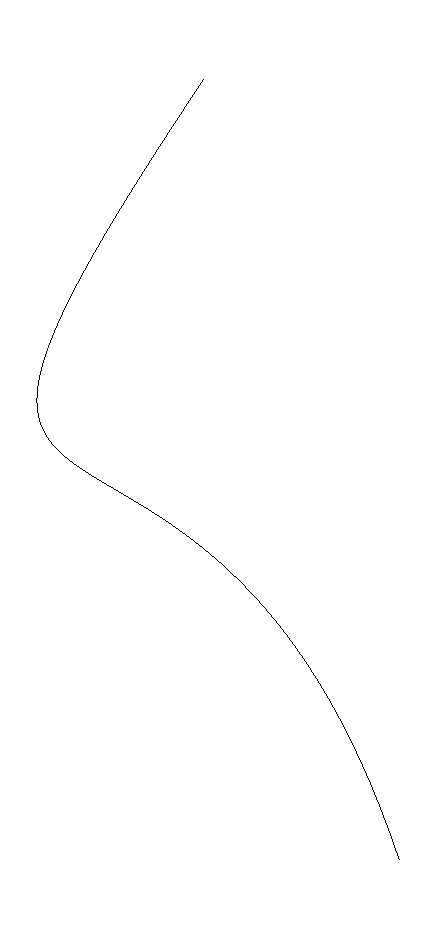
\includegraphics[height=.3\textheight]{graphics/curve_a.pdf}
        \caption{A cubic bezier curve parameterized with the start point $(4,5)$, end point $(3,1)$ and control points $(3,2)$ and $(1,4)$.}
    \end{subfigure}
    \begin{subfigure}{.45\textwidth}
        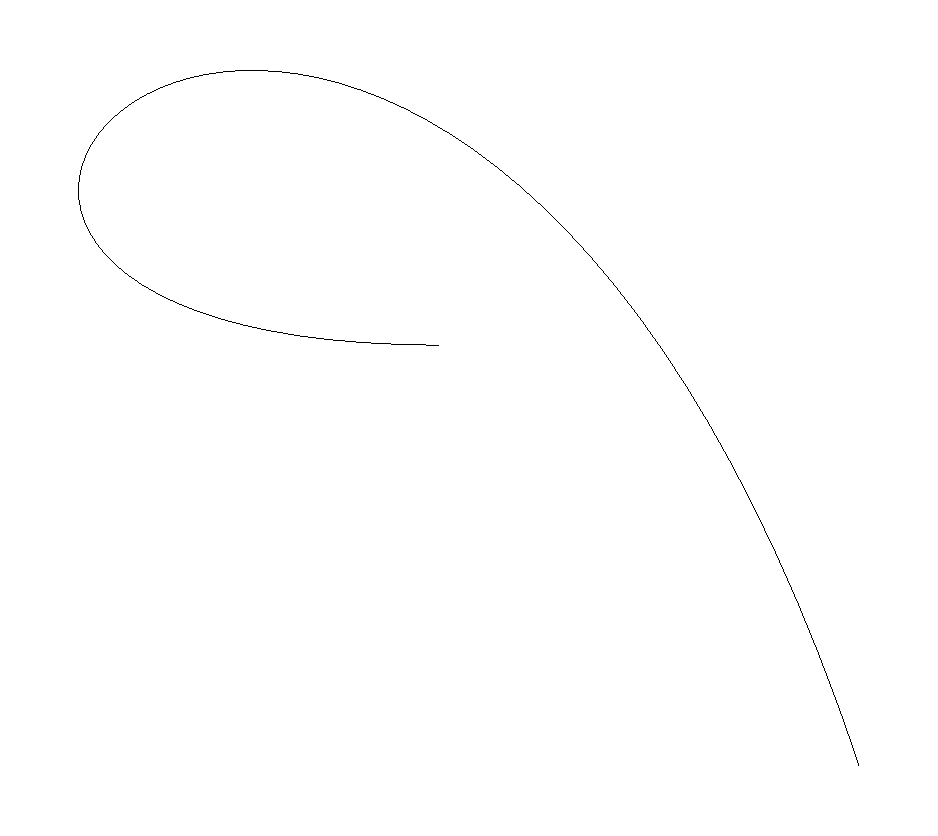
\includegraphics[height=.3\textheight]{graphics/curve_b.pdf}
        \caption{A cubic bezier curve parameterized with the start point $(4,5)$, end point $(3,4)$ and control points $(3,2)$ and $(1,4)$.}
    \end{subfigure}
    \caption{Two cubic bezier curves with identical parameters except the y-coordinate of the end point. Note, that even though nearly all parameters are identical, the visual representation of the curve is completely different.}
    \label{fig:curve.comparison}
\end{figure}

The second consideration for the error function chosen is that the absolute error is used instead of the squared error. This is due to the fact that the squared error diminishes small differences and exaggerates large differences, as described in \Cref{p:losses.regression}. Furthermore, the absolute value is more efficient to compute than the squared value.

As an aside, using the \gls{iou} as error function $d(\hat{\mathbf{y}},\mathbf{y}_j)$ for the total curve error was considered as an additional metric. However, this metric was ultimately not implemented due to high computational requirements.

\paragraph{Curve ratio}
Recall that the output vector image $\hat{\mathbf{Y}}=(\hat{\mathbf{y}}_j)_{j=0}^n$ and the ground truth vector image $\mathbf{Y}=(\mathbf{y}_j)_{j=0}^m$ consist of $n$ and $m$ cubic bezier curves, respectively. Given an output image $\hat{\mathbf{Y}}$ that visually resembles the ground truth $\mathbf{Y}$, a simple measure of matching vector structures is to consider the ratio number of output curves and ground truth curves $n/m\in[0,n]$. In the case of perfectly matching vector structures, $n=m$ and $n/m=1$. In the case of mismatching vector structures, $n/m\neq1$, with values closer to 1 indicating closer matches. Note that this metric should be considered in combination with the \gls{iou}, since it is also possible for the number of curves to match for visually dissimilar images.

\paragraph{Curve length}
The average curve length is an interesting property of vectorization methods, as it shows the kind of primitives the methods are biased towards. The value is calculated by evaluating the cubic bezier curves and measured in pixels. Note that there is no semantic preference towards shorter or longer curves. Hence, it makes sense to consider this information in combination with the average curve length in the ground truth listed in \Cref{tab:gt_metrics}. Values closer to the ground truth can be considered as representing a closer match to the ground truth vector structure. However, the curve length alone is neither sufficient nor necessary to conclude that.

\paragraph{Curve distance}
An important quality of a line-art vector image is that there are no unintended holes between curves. As explained in \Cref{subsec:cleanframes}, unintended holes in clean animation frames increase the difficulty of successive steps in the limited animation process. Furthermore, since junctions can only be represented using coincident curves, having holes in intended junctions can have an adverse effect on downstream applications \citep{Yan:2020:ABR}. Therefore, following \citet{Yan:2020:ABR}, holes between curves are measured using the the minimum distance of each curve endpoints to each other curve endpoints. Similar to \citet{Yan:2020:ABR}, the minimum distances are aggregated by sum instead of the average, since the average would benefit methods that erroneously output short curves with small distances for visually continuous curves in the input image. In detail, given an output vector image $\hat{\mathbf{Y}}=(\hat{\mathbf{y}}_j)_{j=0}^n$, the metric is defined by \Cref{eq:holes.distance}, where $\mathcal{E}=[0,1,6,7]$ defines the indices of the start and the end point parameters of a curve. There exists a small number of outliers with a minimum distance larger than 50 pixels, which are ignored since they are too far removed from other curves to be considered constituting holes within curve sequences.

\begin{equation}
\label{eq:holes.distance}
    \mu_{i=0}^n \left( \min_{j=0}^n \sum_{k\in\mathcal{E}} |\hat{y}_k^i - \hat{y}_k^j| \right)
\end{equation}

Note that there are two limitations associated with this metric. Firstly, it unduly considers some types of curves as having holes. \Cref{fig:intentional.hole} shows that there exist curves which are intentionally not connected to any other curve, but are placed in the close vicinity of other curves. Secondly, the metric does not normalize for the sequence length, which limits comparability since most methods output a different numbers of curves for the same raster image. Hence, as with the curve-length metric, the curve distance has to be considered together with the corresponding ground-truth metric in \Cref{tab:gt_metrics}. The closer the value is to the ground-truth baseline, the closer the vector structure can be considered to match the ground truth, while values that are higher than the baseline indicate more unintentional holes. For values that are smaller than the ground-truth baseline, two interpretations can be considered: If the curve ratio $n/m<1$, it follows that the output vector image simply contains fewer holes in proportion to the curve ratio. Otherwise, it shows that the method outputs fewer unintentional curves than the ground truth, which is unlikely but not impossible, due to the irregularities described in \Cref{subsec:dataset.limitations.irregularities}.

\begin{figure}
    \centering
    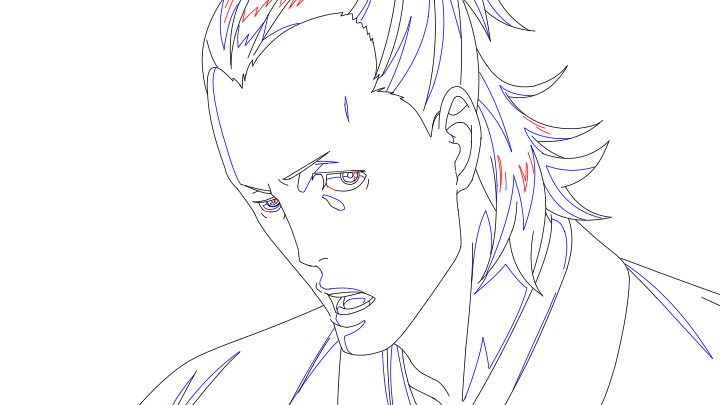
\includegraphics[height=.25\textheight,trim={17em 7em 25em 14em},clip]{graphics/douga/49.pdf}
    \caption{The clean animation frame shown in \Cref{fig:clean-frame-vec} zoomed into the nose region, which contains intentionally unconnected curves. Such curves include the black curve representing the right nostril, the black curve representing the upper lip or the black curve representing the crinkle below the left eye.}
    \label{fig:intentional.hole}
\end{figure}

\paragraph{Runtime}
A metric only tangentially related to the correct vectorization of a raster image, but still important for the application of the vectorization method is the runtime required to produce a vector image. The metric is measured in seconds, with lower values indicating faster algorithms. The runtime is measured using GNU Time \citep{gnutime} by adding the \gls{cpu} time spent in the kernel and in the user mode. An alternative would be to take the wall clock time, i.e., the total elapsed time between start and finish of the process. However, this value is not used since it could be inconsistently influenced by other processes blocking required resources.

\paragraph{\gls{gpu} Memory usage}
Another performance metric only tangentially related to the correct vectorization of a raster image is the maximum amount of dedicated \gls{gpu} memory required by the process. This is important since dedicated \gls{gpu} memory is often a limiting factor. It is measured using the \texttt{nvidia-smi} tool in \gls{mib}, where lower values indicate less memory usage. It is not measured for AutoTrace \citep{autotrace} since it does not use the \gls{gpu}.


Another important characteristic of output vector images is the number of overlapping curves, which could be calculated  similar to \Cref{subsec:dataset.stats}. However, since the calculation of overlapping curves is computationally expensive, this metric was not considered. Furthermore, overlapping curves are less of an issue than holes between curves, as described in \Cref{sec:challenges}.

Each performance metric is calculated per curve, leading to a metric distribution over all curves for each image in the test dataset. The two exceptions to this are the \gls{iou} and the runtime, which are calculated per image, leading to a distribution over all images in the test dataset. In any case, these distributions are represented using aggregate measures for location and skew. Usually, the mean and standard deviation are used for this purpose. However, these measures have low statistical efficiency when applied to non-normal data. \Cref{fig:example.metric.distributions} shows the distributions for the metrics of the line-art vectorization method developed in this work applied to the image shown in \Cref{fig:input.output.example}. It can be seen that the distributions do not follow the normal distribution, as they are left-skewed and contain outliers. This is corroborated by applying the Shapiro-Wilk test \citep{10.1093/biomet/52.3-4.591} on the data, which yields a p-value lower than 0.05 for all distributions, thereby rejecting the null hypothesis that the samples were drawn from the normal distribution. Thus, the median and the \gls{iqr} are chosen as robust alternatives for the location and skew measure. The only exception is the \gls{iou} shown in \Cref{fig:example.metric.distributions.raster_dist}, which is reasonably normal distributed. Still, to keep metrics consistent, the median and \gls{iqr} are used as aggregate measures for the \gls{iou} as well.

The metric distributions and other distributions are often compared against each other in subsequent sections, e.g. when comparing differences in model performance. In order to ascertain whether differences are actually statistically significant, the Wilcoxon-Mann-Whitney U-Test \citep{c4091bd3-d888-3152-8886-c284bf66a93a,10.1214/aoms/1177730491} is used. This test is used because it is nonparametric and has relaxed assumptions of the underlying distribution. The null hypothesis $H_0$ is that the model metrics follow the same distribution. The alternative hypothesis $H_A$ is that they follow different distributions. The primary interest lies in the \textit{location} of the distributions. The output of the statistical test is a $p$-value, which indicates the probability of the observed sample given the assumption of $H_0$ being true. Under the assumption of a significance level of $\alpha=95\%=0.95$, if $p < 1-\alpha=0.05$, $H_0$ is rejected and $H_A$ is accepted. This setup is used throughout the text when statistical significance is mentioned.

\begin{figure}[h]
    \centering
    \begin{subfigure}{.3\textwidth}
        \includegraphics[width=\textwidth]{graphics/eval/curve_error.pdf}
        \caption{Distribution of the curve error.}
        \label{fig:example.metric.distributions.curve_error}
    \end{subfigure}
    \begin{subfigure}{.3\textwidth}
        \includegraphics[width=\textwidth]{graphics/eval/curve_length.pdf}
        \caption{Distribution of the curve length.}
        \label{fig:example.metric.distributions.curve_length}
    \end{subfigure}
    \begin{subfigure}{.3\textwidth}
        \includegraphics[width=\textwidth]{graphics/eval/min_dist.pdf}
        \caption{Distribution of the minimum curve distance.}
        \label{fig:example.metric.distributions.min_dist}
    \end{subfigure}
    \begin{subfigure}{.3\textwidth}
        \includegraphics[width=\textwidth]{graphics/eval/raster_dist.pdf}
        \caption{Distribution of the \gls{iou} for all images in the Tonari test set.}
        \label{fig:example.metric.distributions.raster_dist}
    \end{subfigure}
    \begin{subfigure}{.3\textwidth}
        \includegraphics[width=\textwidth]{graphics/eval/curve_ratio.pdf}
        \caption{Distribution of the curve ratio for all images in the Tonari test set.}
        \label{fig:example.metric.distributions.curve_ratio}
    \end{subfigure}
    \begin{subfigure}{.3\textwidth}
    \includegraphics[width=\textwidth]{graphics/eval/runtime.pdf}
        \caption{Distribution of the runtime for all images in the Tonari test set.}
        \label{fig:example.metric.distributions.runtime}
    \end{subfigure}
    \caption{The distributions of all metrics calculated for the line-art image vectorization method developed in this work. The top three metrics are calculated for the image shown in \Cref{fig:input.output.example}. The bottom three metrics are calculated for the entire Tonari test dataset.}
    \label{fig:example.metric.distributions}
\end{figure}

\clearpage
\subsection{Quantitative Evaluation}
\label{subsec:eval.quant}
To answer the \gls{rq1}, this section provides a quantitative evaluation of the extent to which the line-art vectorization method developed in this work and related state-of-the-art methods are able to automatically vectorize clean animation frames. For this purpose, the methods are applied to vectorize a test dataset consisting of these images. Using the metrics described in \Cref{subsec:eval.metrics}, it is possible to ascertain and compare the results of the methods.

\begin{table}[]
    \centering
    \begin{tabular}{llrrrrrr}
\toprule
 &  & \multicolumn{2}{c}{curves} & \multicolumn{2}{c}{curve length} & \multicolumn{2}{c}{curve distance} \\
 &  & median & \acrshort{iqr} & median & \acrshort{iqr} & median & \acrshort{iqr} \\
\midrule
\multirow[t]{2}{*}{tonari} & 512-0.512 & 205.00 & 423.00 & 2.56 & 0.79 & 1555.82 & 1832.41 \\
 & 1024-1.024 & 205.00 & 423.00 & 5.12 & 1.57 & 1725.81 & 3489.33 \\
\cline{1-8}
\multirow[t]{2}{*}{sketchbench} & 512-0.512 & 208.00 & 266.00 & 12.43 & 14.29 & 2355.22 & 1237.41 \\
 & 1024-1.024 & 208.00 & 266.00 & 24.85 & 28.57 & 2726.03 & 2330.49 \\
\cline{1-8}
\bottomrule
\end{tabular}

    \caption{Selected metrics of the vector images in the test dataset. This information can be used as baseline for the corresponding metrics in \Cref{tab:tonari-False-512-0.512}. Note that the ground truth images are scaled to all evaluation resolutions to produce baseline values in all resolutions for convenience.}
    \label{tab:gt_metrics}
\end{table}
    
\begin{table}[h]
    \centering
    \begin{tabular}{lllllll}
\toprule
 &  & autotrace & \parbox[]{5em}{polyvector-\\flow} & \parbox[]{4em}{virtual-\\sketching} & \parbox[]{4em}{deepvec-\\techdraw} & marked \\
\midrule
\multirow[t]{2}{*}{\acrshort{iou} $\uparrow$} & median & 0.02 & 0.12 & \textit{0.29} & 0.28 & \textbf{0.30} \\
 & \acrshort{iqr} & 0.01 & 0.11 & 0.06 & 0.07 & 0.05 \\
\cline{1-7}
\multirow[t]{2}{*}{curve ratio} & median & 0.23 & 1.35 & 0.30 & 0.19 & 0.43 \\
 & \acrshort{iqr} & 0.11 & 1.08 & 0.14 & 0.13 & 0.15 \\
\cline{1-7}
\multirow[t]{2}{*}{curve length} & median & 1.00 & 0.55 & 11.16 & 9.06 & 8.19 \\
 & \acrshort{iqr} & 0.41 & 0.04 & 4.18 & 2.10 & 2.45 \\
\cline{1-7}
\multirow[t]{2}{*}{curve distance} & median & 891.00 & 439.18 & 1442.91 & 917.50 & 1361.28 \\
 & \acrshort{iqr} & 1535.00 & 1126.02 & 1782.80 & 974.06 & 1498.03 \\
\cline{1-7}
\multirow[t]{2}{*}{curve error $\downarrow$} & median & 20.37 & \textbf{14.05} & 20.08 & 17.58 & \textit{16.76} \\
 & \acrshort{iqr} & 19.15 & 14.64 & 9.12 & 10.03 & 5.36 \\
\cline{1-7}
\multirow[t]{2}{*}{runtime $\downarrow$} & median & \textbf{0.35} & 14.82 & 22.99 & 97.73 & \textit{9.49} \\
 & \acrshort{iqr} & 0.31 & 23.95 & 7.34 & 72.20 & 13.18 \\
\cline{1-7}
\bottomrule
\end{tabular}

    \caption{Comparison of the performance of the marked line-art image vectorization method and four prior works on the Tonari test subset at a resolution of 512px. If possible, the result of the best and the second-best performing method for the metric is indicated using bold and italics fonts, respectively.}
    \label{tab:tonari-False-512-0.512}
\end{table}

\begin{table}[!h]
    \centering
    \begin{tabular}{lllllll}
\toprule
 &  & autotrace & \parbox[]{5em}{polyvector-\\flow} & \parbox[]{4em}{virtual-\\sketching} & \parbox[]{4em}{deepvec-\\techdraw} & marked \\
\midrule
\multirow[t]{2}{*}{\acrshort{iou} $\uparrow$} & median & 0.02 & 0.09 & \textit{0.27} & 0.27 & \textbf{0.30} \\
 & \acrshort{iqr} & 0.01 & 0.05 & 0.04 & 0.05 & 0.05 \\
\cline{1-7}
\multirow[t]{2}{*}{curve ratio} & median & 1.01 & 3.47 & 1.00 & 0.71 & 1.36 \\
 & \acrshort{iqr} & 0.83 & 1.35 & 0.77 & 0.46 & 0.72 \\
\cline{1-7}
\multirow[t]{2}{*}{curve length} & median & 1.00 & 0.55 & 14.27 & 9.70 & 11.38 \\
 & \acrshort{iqr} & 0.41 & 0.03 & 2.00 & 2.78 & 4.01 \\
\cline{1-7}
\multirow[t]{2}{*}{curve distance} & median & 2359.00 & 863.19 & 2619.79 & 1533.96 & 2549.28 \\
 & \acrshort{iqr} & 641.00 & 1179.56 & 482.01 & 387.16 & 958.53 \\
\cline{1-7}
\multirow[t]{2}{*}{curve error $\downarrow$} & median & 50.82 & \textbf{39.73} & 51.01 & \textit{42.18} & 46.72 \\
 & \acrshort{iqr} & 31.58 & 44.97 & 29.90 & 22.00 & 37.58 \\
\cline{1-7}
\multirow[t]{2}{*}{runtime $\downarrow$} & median & \textbf{0.43} & 25.41 & 28.00 & 121.91 & \textit{15.83} \\
 & \acrshort{iqr} & 0.20 & 24.78 & 3.87 & 36.39 & 16.14 \\
\cline{1-7}
\bottomrule
\end{tabular}

    \caption{Comparison of the performance of the marked line-art image vectorization method and four prior works on the SketchBench test subset at a resolution of 512px.}
    \label{tab:sketchbench-False-512-0.512}
\end{table}

\begin{table}[]
    \centering
    \begin{tabular}{l|r}
        method & memory $\downarrow$ \\
        \hline
        polyvector-flow & \textit{1128} \\
        virtual-sketching & 2760 \\
        deepvectechdraw & 1935 \\
        marked & \textbf{1008}
    \end{tabular}
    \caption{Maximum dedicated \gls{gpu} memory measured in \gls{mib} required by the deep learning-based line-art image vectorization methods.}
    \label{tab:max_memory}
\end{table}

\Cref{tab:tonari-False-512-0.512} shows the performance of the following line-art image vectorization methods:

\begin{itemize}
    \item The method developed in this work, identified as \texttt{marked},
    \item The traditional algorithm by \citet{autotrace}, identified as \texttt{autotrace},
    \item The vectorization algorithm combining deep learning and heuristic optimization by \citet{Puhachov2021KeypointPolyvector} identified as \texttt{polyvector-flow},
    \item The deep learning-based algorithm using raster supervision by \citet{mo2021virtualsketching}, identified as \texttt{virtual-sketching}, and
    \item The deep learning-based algorithm using vector supervision by \citet{DBLP:conf/eccv/EgiazarianVAVST20}, identified by \texttt{deepvectechdraw}.
\end{itemize}

The methods are applied on the Tonari clean animation frame test dataset rasterized at a resolution of 512px, while preserving the aspect ratio (see \Cref{subsec:dataset.processing}). The performance is measured according using metrics explained in \Cref{subsec:eval.metrics}. Recall that the average curve length and the average curve distance should be close to the ground truth values, which are listed in \Cref{tab:gt_metrics}. The curve ratio is calculated with the number of curves listed in the same table. For the remaining metrics, the results can be interpreted more easily. While the arrow in the column name indicates whether larger or smaller numbers represent better performance, the results of the best and the second-best performing method on the metric are indicated using bold and italics fonts, respectively.

\Cref{tab:tonari-False-512-0.512} shows that the line-art vectorization method developed in this work outputs vector images that resemble the input raster image the closest. It achieves this with the second-smallest curve error behind the method by \citet{Puhachov2021KeypointPolyvector} and with a curve distance that is close to the ground truth, just behind the method by \citet{mo2021virtualsketching}. Interestingly, it uses roughly half the curves of the ground truth, with curves on average being nearly twice as long. Finally, it is also the fastest deep learning-based method, while requiring the least amount of dedicated \gls{gpu} memory (see \Cref{tab:max_memory}).


Note that the traditional method by \citet{autotrace} significantly outperforms all other methods on the runtime. On the other hand, it has the highest curve error and lowest \gls{iou}, suggesting ill-fitting outputs. The method by \citet{Puhachov2021KeypointPolyvector} also achieves a surprisingly low \gls{iou}, but also the best curve error. Note, that the output images of this method contain significantly more curves than other methods due to the overparamterezied outputs mentioned in \Cref{p:eval.setup.prior.poly}. This leads to a low curve distance, since most curves are just splitted parts of a long polyline.

The other two deep learning-based methods by \citet{mo2021virtualsketching,DBLP:conf/eccv/EgiazarianVAVST20} approach the \gls{iou} of the method developed in this work, albeit with a significantly higher curve error and runtime. Additionally, the method by \citet{DBLP:conf/eccv/EgiazarianVAVST20} outputs the lowest amounts of curves, but the curves of the method by \citet{mo2021virtualsketching} are still longer on average, suggesting that this method produces more curves that do not fit the ground truth curves.

\Cref{tab:sketchbench-False-512-0.512} shows that similar results are maintained on the publicly available SketchBench test dataset, demonstrating reproducibility and generalizability of the evaluation. Unsurprisingly, since the SketchBench images in general contain significantly fewer curves than Tonari images (see \Cref{subsec:dataset.stats}), the curve ratio ends up significantly higher.

In general, recall that the \gls{iou} is in $[0,1]$. Hence, most methods produce output images that surprisingly do not cover the input image well. This suggests that no method reproduces clean animation frames to the extent required by the task considered in this work.
\clearpage
\subsubsection{Results with higher resolution input images}
\label{subsec:eval.quant.1024}

\begin{table}[h]
    \centering
    \begin{tabular}{lllllll}
\toprule
 &  & autotrace & \parbox[]{5em}{polyvector-\\flow} & \parbox[]{4em}{virtual-\\sketching} & \parbox[]{4em}{deepvec-\\techdraw} & marked \\
\midrule
\multirow[t]{2}{*}{\acrshort{iou} $\uparrow$} & median & 0.01 & \textbf{0.67} & 0.49 & \textit{0.52} & 0.31 \\
 & \acrshort{iqr} & 0.00 & 0.05 & 0.04 & 0.14 & 0.04 \\
\cline{1-7}
\multirow[t]{2}{*}{curve ratio} & median & 0.27 & 17.49 & 0.63 & 0.32 & 0.39 \\
 & \acrshort{iqr} & 0.14 & 5.93 & 0.15 & 0.13 & 0.11 \\
\cline{1-7}
\multirow[t]{2}{*}{curve length} & median & 1.41 & 0.50 & 14.81 & 17.39 & 15.75 \\
 & \acrshort{iqr} & 0.41 & 0.02 & 2.17 & 4.80 & 4.83 \\
\cline{1-7}
\multirow[t]{2}{*}{curve distance} & median & 954.00 & 5068.26 & 2999.09 & 1622.45 & 1745.01 \\
 & \acrshort{iqr} & 2091.00 & 7893.17 & 4545.06 & 1669.95 & 2070.26 \\
\cline{1-7}
\multirow[t]{2}{*}{curve error $\downarrow$} & median & 31.99 & 33.99 & \textit{31.52} & \textbf{28.81} & 34.76 \\
 & \acrshort{iqr} & 25.92 & 38.28 & 20.31 & 12.80 & 18.17 \\
\cline{1-7}
\multirow[t]{2}{*}{runtime $\downarrow$} & median & \textbf{1.48} & 113.41 & 38.21 & 136.90 & \textit{9.46} \\
 & \acrshort{iqr} & 0.25 & 244.59 & 27.34 & 164.06 & 10.48 \\
\cline{1-7}
\bottomrule
\end{tabular}

    \caption{The same comparison as \Cref{fig:res_comparison} with input images of resolution 1024px.}
    \label{tab:tonari-False-1024-1.024}
\end{table}

\begin{table}[h]
    \centering
    \begin{tabular}{lllllll}
\toprule
 &  & autotrace & \parbox[]{5em}{polyvector-\\flow} & \parbox[]{4em}{virtual-\\sketching} & \parbox[]{4em}{deepvec-\\techdraw} & marked \\
\midrule
\multirow[t]{2}{*}{\acrshort{iou} $\uparrow$} & median & 0.01 & \textbf{0.74} & 0.50 & \textit{0.58} & 0.30 \\
 & \acrshort{iqr} & 0.00 & 0.04 & 0.03 & 0.07 & 0.03 \\
\cline{1-7}
\multirow[t]{2}{*}{curve ratio} & median & 1.11 & 78.40 & 2.47 & 0.97 & 1.31 \\
 & \acrshort{iqr} & 0.55 & 58.65 & 1.15 & 0.46 & 0.77 \\
\cline{1-7}
\multirow[t]{2}{*}{curve length} & median & 1.41 & 0.52 & 16.99 & 26.60 & 23.40 \\
 & \acrshort{iqr} & 0.00 & 0.01 & 1.72 & 11.05 & 7.68 \\
\cline{1-7}
\multirow[t]{2}{*}{curve distance} & median & 2390.00 & 12440.78 & 7069.76 & 2540.16 & 2680.15 \\
 & \acrshort{iqr} & 1291.00 & 5584.74 & 3125.29 & 1886.62 & 1642.49 \\
\cline{1-7}
\multirow[t]{2}{*}{curve error $\downarrow$} & median & 102.56 & 109.27 & 94.82 & \textbf{72.07} & \textit{93.62} \\
 & \acrshort{iqr} & 47.00 & 56.38 & 55.52 & 33.63 & 72.84 \\
\cline{1-7}
\multirow[t]{2}{*}{runtime $\downarrow$} & median & \textbf{1.84} & 280.16 & 56.01 & 300.92 & \textit{15.73} \\
 & \acrshort{iqr} & 0.44 & 132.90 & 17.81 & 186.96 & 13.91 \\
\cline{1-7}
\bottomrule
\end{tabular}

    \caption{The same comparison as \Cref{tab:tonari-False-1024-1.024} on the SketchBench test dataset instead of the Tonari test dataset.}
    \label{tab:sketchbench-False-1024-1.024}
\end{table}

The methods by \citet{autotrace,Puhachov2021KeypointPolyvector} performed unusually low on the evaluation in \Cref{tab:tonari-False-512-0.512}. A potential cause for this was identified as the low resolution of input images at 512px. To ascertain this hypothesis, the evaluation was rerun with input images rasterized at twice the resolution, i.e., 1024px, while preserving the aspect ratio. Note that this does not affect the training of the marked-curve reconstruction model, i.e. the model trained on a resolution of 512px is used. Keep in mind that this is significantly higher than the standard resolution of clean animation frames considered in this work (see \Cref{subsec:dataset.douga}). Hence, performance increases of methods at this resolution will likely not materialize when they are applied to real-world clean animation frames, which likely will only be available at a lower resolution.

\Cref{tab:tonari-False-1024-1.024} shows the evaluation results on higher resolution. Note that the metrics measured in pixels are affected by the increased resolution, i.e., given an identical vector structure, a curve error of 20px at 512px resolution corresponds to 40px at 1024px resolution. It is clear that all prior methods except AutoTrace \citep{autotrace} perform significantly better than at 512px resolution. The method by \citet{Puhachov2021KeypointPolyvector} even reaches an \gls{iou} well over 0.5, i.e., its outputs cover more than half of the input image correctly on average. This is dampened by a high curve error and curve distance, indicating incorrect vector structures. The method by \citet{DBLP:conf/eccv/EgiazarianVAVST20} performs similarly well, with a lower \gls{iou} but better curve error and curve distance, seemingly striking a different balance between visual resemblance and semantically correct vector structures.

Interestingly, the metrics of the method developed in this work stay remarkably stable at the increased resolution. This intriguing property is investigated in \Cref{fig:res_comparison}, which shows the differences of metrics at both resolution sizes. Note that, since metrics measured in pixels scale linearly with the resolution size, they are normalized by the resolution size, i.e., the values of metrics measured at the resolution of 1024px are divided by 2. The method developed in this work is the only one for which metrics do not significantly change depending on the input image resolution. This is especially remarkable for the runtime, which significantly and predictably changes for all other methods. The only exception to this is the curve error and the curve distance, which significantly increases only for the method by \citet{Puhachov2021KeypointPolyvector}. Since the increase in curve distance of this method is especially drastic, it cannot be displayed in \Cref{fig:curve_distance_res}. Furthermore, the \gls{iou} and curve ratio of AutoTrace \citep{autotrace} and the curve length of the method by \citet{DBLP:conf/eccv/EgiazarianVAVST20} do not change significantly. Also of interest is that the curve length of the method by \citet{mo2021virtualsketching} actually significantly decreases at high resolutions.

\Cref{tab:sketchbench-False-1024-1.024,fig:res_comparison.sketchbench} show that similar results are maintained on the SketchBench test dataset, with the curve error of the method developed in this work slightly improving against other methods.

One potential reason for this remarkable input image resolution invariance of the method developed in this work is the selection of reconstruction curves using marks, which explicitly \emph{forces} the model to reconstruct curves which other methods might not have detected. This can be the case for curves that are too thin or contain some spots at low resolutions.

While other methods achieve significantly better results at the high resolution of 1024px, it needs to be kept in mind that this resolution is higher than the target resolution of clean animation frames by Tonari Animation. Hence, these high results might not materialize when used for real-world data. One potential way to maintain this good performance of other methods with input images at lower resolutions is to apply super-resolution models \citep{DBLP:journals/pami/DongLHT16} to the input images. However, these models would need to be successfully finetuned to high-resolution line-art images beforehand, which is an open research question on its own.

An interesting question is if this trend continues at even lower resolutions. However, this was not attempted, because resolutions that are significantly lower than 512px are unreasonable small to still expect methods to extract semantically meaningful information out of input images.

\begin{figure}[h]
    \centering
    \begin{subfigure}{.3\textwidth}
    \centering
    \includegraphics[width=\textwidth]{graphics/eval/iou_res.pdf}
    \caption{The average \gls{iou}.}
    \label{fig:iou_res}
\end{subfigure}
    \begin{subfigure}{.3\textwidth}
    \centering
    \includegraphics[width=\textwidth]{graphics/eval/curve_ratio_res.pdf}
    \caption{The average curve ratio.}
\end{subfigure}
    \begin{subfigure}{.3\textwidth}
    \centering
    \includegraphics[width=\textwidth]{graphics/eval/runtime_res.pdf}
    \caption{The average runtime.}
\end{subfigure}
    \begin{subfigure}{.3\textwidth}
    \centering
    \includegraphics[width=\textwidth]{graphics/eval/curve_length_res.pdf}
    \caption{The average curve length.}
\end{subfigure}
    \begin{subfigure}{.3\textwidth}
    \centering
    \includegraphics[width=\textwidth]{graphics/eval/curve_distance_res.pdf}
    \caption{The total curve distance.}
    \label{fig:curve_distance_res}
\end{subfigure}
    \begin{subfigure}{.3\textwidth}
    \centering
    \includegraphics[width=\textwidth]{graphics/eval/curve_error_res.pdf}
    \caption{The average curve error.}
\end{subfigure}
    \caption{Metrics for the line-art image vectorization methods evaluated on images with 512px and 1024px resolution, respectively. Points denote the median of the metric, while vertical bars denote the \gls{iqr}. Horizontal lines show the trend of the metric. The metrics for the method developed in this work are emphasized. Note that they are not significantly affected by the image resolution and none decreases with lower resolutions.}
    \label{fig:res_comparison}
\end{figure}

\begin{figure}[!h]
    \centering
    \begin{subfigure}{.3\textwidth}
    \centering
    \includegraphics[width=\textwidth]{graphics/eval/iou_res_sketchbench.pdf}
    \caption{The average \gls{iou}.}
    \label{fig:iou_res_sketchbench}
\end{subfigure}
    \begin{subfigure}{.3\textwidth}
    \centering
    \includegraphics[width=\textwidth]{graphics/eval/curve ratio_res_sketchbench.pdf}
    \caption{The average curve ratio.}
\end{subfigure}
    \begin{subfigure}{.3\textwidth}
    \centering
    \includegraphics[width=\textwidth]{graphics/eval/runtime_res_sketchbench.pdf}
    \caption{The average runtime.}
\end{subfigure}
    \begin{subfigure}{.3\textwidth}
    \centering
    \includegraphics[width=\textwidth]{graphics/eval/curve length_res_sketchbench.pdf}
    \caption{The average curve length.}
\end{subfigure}
    \begin{subfigure}{.3\textwidth}
    \centering
    \includegraphics[width=\textwidth]{graphics/eval/curve distance_res_sketchbench.pdf}
    \caption{The total curve distance.}
    \label{fig:curve_distance_res_sketchbench}
\end{subfigure}
    \begin{subfigure}{.3\textwidth}
    \centering
    \includegraphics[width=\textwidth]{graphics/eval/curve error_res_sketchbench.pdf}
    \caption{The average curve error.}
\end{subfigure}
    \caption{The same comparison as in \Cref{fig:res_comparison} on the SketchBench test dataset instead of the Tonari test dataset.}
    \label{fig:res_comparison.sketchbench}
\end{figure}

\clearpage
\subsubsection{Results with binarized input images}
\label{subsec:eval.quant.True}

Looking at the results with higher resolution input images, one can assume that the cause for the bad performance of the methods by \citet{autotrace,Puhachov2021KeypointPolyvector} in \Cref{tab:tonari-False-512-0.512} is that the raster input images are not clearly visible enough. One way to improve this is to binarize the image with a low threshold for black pixels, which accentuates curves. In order to investigate this assumption, the evaluation was rerun using binarized input images. \Cref{tab:tonari-True-512-0.512,fig:binarization_comparison} show that the curve ratio significantly increases for the method by \citet{Puhachov2021KeypointPolyvector} and the curve length significantly increases for both methods, thus corroborating the assumption. This leads to the \gls{iou} significantly improving for both methods, with the method by \citet{Puhachov2021KeypointPolyvector} even surpassing the method developed in this work. Furthermore, the method now achieves the lowest curve error, while the improved curve error of AutoTrace \citep{autotrace} is still the worst value of all methods. On the other hand, the curve distance significantly worsens for the method by \citet{Puhachov2021KeypointPolyvector}, showing that the low value for non-binarized input images is just an artifact of output images containing a small amount of curves in the first place.

\begin{table}[h]
    \centering
    \begin{tabular}{lllllll}
\toprule
 &  & autotrace & \parbox[]{5em}{polyvector-\\flow} & \parbox[]{4em}{virtual-\\sketching} & \parbox[]{4em}{deepvec-\\techdraw} & marked \\
\midrule
\multirow[t]{2}{*}{\acrshort{iou} $\uparrow$} & median & 0.17 & \textbf{0.39} & \textit{0.29} & 0.18 & 0.28 \\
 & \acrshort{iqr} & 0.04 & 0.05 & 0.02 & 0.08 & 0.04 \\
\cline{1-7}
\multirow[t]{2}{*}{curve ratio} & median & 0.27 & 7.32 & 0.40 & 0.13 & 0.44 \\
 & \acrshort{iqr} & 0.11 & 2.01 & 0.13 & 0.09 & 0.22 \\
\cline{1-7}
\multirow[t]{2}{*}{curve length} & median & 9.43 & 0.50 & 10.37 & 9.92 & 7.99 \\
 & \acrshort{iqr} & 4.39 & 0.04 & 3.77 & 4.87 & 3.19 \\
\cline{1-7}
\multirow[t]{2}{*}{curve distance} & median & 1230.46 & 2453.15 & 1723.93 & 593.07 & 1413.85 \\
 & \acrshort{iqr} & 1188.55 & 3520.67 & 1926.67 & 498.94 & 1677.94 \\
\cline{1-7}
\multirow[t]{2}{*}{curve error $\downarrow$} & median & 19.81 & \textbf{16.26} & 19.77 & 20.52 & \textit{17.68} \\
 & \acrshort{iqr} & 11.03 & 9.61 & 11.32 & 30.64 & 5.68 \\
\cline{1-7}
\multirow[t]{2}{*}{runtime $\downarrow$} & median & \textbf{0.03} & 59.22 & 22.92 & 79.59 & \textit{9.76} \\
 & \acrshort{iqr} & 0.01 & 117.67 & 9.47 & 33.39 & 11.42 \\
\cline{1-7}
\bottomrule
\end{tabular}

    \caption{The same comparison as \Cref{tab:tonari-False-512-0.512} with binarization of images applied prior to running the methods.}
    \label{tab:tonari-True-512-0.512}
\end{table}

However, it can also be seen that binarization is not a silver bullet, as the method by \citet{DBLP:conf/eccv/EgiazarianVAVST20} is actively harmed by it. With binarized input images, it has a significantly worse \gls{iou} and a worse curve error.

Interestingly, the changes in curve error are not statistically significant for any method. The methods by \citet{autotrace,Puhachov2021KeypointPolyvector} have a significantly higher runtime than with non-binarized input images, further corroborating that they detect and reconstruct more  curves given binarized input images. Furthermore, the curve ratio of the method by \citet{mo2021virtualsketching} significantly increases. Other than that, most metrics do not change significantly.

Again, the metrics for the method developed in this work remain remarkably stable on binarized and non-binarized input images, with none changing significantly. Together with the similar result on resolution invariance, this shows that the method developed in this work is more robust to thinner and potentially poorly visible curves, as it is \emph{forced} to reconstruct them when they are marked. Furthermore, the \gls{iou} and curve error are only beaten by the method by \citet{Puhachov2021KeypointPolyvector}.

\begin{table}[h]
    \centering
    \begin{tabular}{lllllll}
\toprule
 &  & autotrace & \parbox[]{5em}{polyvector-\\flow} & \parbox[]{4em}{virtual-\\sketching} & \parbox[]{4em}{deepvec-\\techdraw} & marked \\
\midrule
\multirow[t]{2}{*}{\acrshort{iou} $\uparrow$} & median & 0.16 & \textbf{0.41} & 0.29 & 0.18 & \textit{0.30} \\
 & \acrshort{iqr} & 0.03 & 0.02 & 0.01 & 0.07 & 0.05 \\
\cline{1-7}
\multirow[t]{2}{*}{curve ratio} & median & 0.72 & 33.38 & 1.63 & 0.40 & 1.35 \\
 & \acrshort{iqr} & 0.40 & 27.34 & 0.91 & 0.53 & 0.77 \\
\cline{1-7}
\multirow[t]{2}{*}{curve length} & median & 20.42 & 0.52 & 13.89 & 12.32 & 11.91 \\
 & \acrshort{iqr} & 8.20 & 0.02 & 1.39 & 2.91 & 3.24 \\
\cline{1-7}
\multirow[t]{2}{*}{curve distance} & median & 1841.21 & 5900.94 & 3300.44 & 1130.48 & 2512.57 \\
 & \acrshort{iqr} & 883.82 & 2639.11 & 1414.49 & 436.67 & 875.13 \\
\cline{1-7}
\multirow[t]{2}{*}{curve error $\downarrow$} & median & \textbf{40.02} & 55.18 & 48.54 & 57.22 & \textit{46.66} \\
 & \acrshort{iqr} & 12.44 & 28.78 & 24.91 & 24.86 & 36.51 \\
\cline{1-7}
\multirow[t]{2}{*}{runtime $\downarrow$} & median & \textbf{0.04} & 136.89 & 27.13 & 159.14 & \textit{16.79} \\
 & \acrshort{iqr} & 0.00 & 78.87 & 5.36 & 49.33 & 13.88 \\
\cline{1-7}
\bottomrule
\end{tabular}

    \caption{The same comparison as \Cref{tab:tonari-True-512-0.512} on the SketchBench test dataset instead of the Tonari test dataset.}
    \label{tab:sketchbench-True-512-0.512}
\end{table}

\Cref{tab:sketchbench-True-512-0.512,fig:binarization_comparison.sketchbench} show that the results hold on the SketchBench test dataset, with the exception of the curve error, which actually significantly worsens for the method by \citet{Puhachov2021KeypointPolyvector}.

In general, while the results of the methods by \citet{Puhachov2021KeypointPolyvector,autotrace} significantly improve by using binarized input images, this also shows that these methods depend on a high signal-to-noise ratio in the input image. As has been shown, this is easy to achieve for clean line-art images considered in this work by simply binarizing them using a high threshold. However, binarization is non-trivial for images from different domains, which would be the input in a possible cross-domain extension of the line-art vectorization method, as explained in \Cref{sec:challenges}. Under this assumption, methods that are more robust to non-binarized images (and therefore to a lower signal-to-noise ratio) can be considered more suited for a possible extension to cross-domain line-art image vectorization. On the other hand, similar to the super-resolution case mentioned in \Cref{subsec:eval.quant.1024}, this can also be solved by training a separate binarization model for the specific domain, which could be applied before using the images as inputs to the methods by \citet{Puhachov2021KeypointPolyvector,autotrace}.

\begin{figure}[h]
    \centering
    \begin{subfigure}{.3\textwidth}
    \centering
    \includegraphics[width=\textwidth]{graphics/eval/iou_binarization_tonari.pdf}
    \caption{The average \gls{iou}.}
\end{subfigure}
    \begin{subfigure}{.3\textwidth}
    \centering
    \includegraphics[width=\textwidth]{graphics/eval/curve ratio_binarization_tonari.pdf}
    \caption{The average curve ratio.}
\end{subfigure}
    \begin{subfigure}{.3\textwidth}
    \centering
    \includegraphics[width=\textwidth]{graphics/eval/runtime_binarization_tonari.pdf}
    \caption{The average runtime.}
\end{subfigure}
    \begin{subfigure}{.3\textwidth}
    \centering
    \includegraphics[width=\textwidth]{graphics/eval/curve length_binarization_tonari.pdf}
    \caption{The average curve length.}
\end{subfigure}
    \begin{subfigure}{.3\textwidth}
    \centering
    \includegraphics[width=\textwidth]{graphics/eval/curve distance_binarization_tonari.pdf}
    \caption{The total curve distance.}
\end{subfigure}
    \begin{subfigure}{.3\textwidth}
    \centering
    \includegraphics[width=\textwidth]{graphics/eval/curve error_binarization_tonari.pdf}
    \caption{The average curve error.}
\end{subfigure}
    \caption{Metrics for the line-art image vectorization methods evaluated on binarized and non-binarized images with 512px resolution, respectively. Points denote the median of the metric, while vertical bars denote the \gls{iqr}. The metrics for the method developed in this work are emphasized. Note that they are not significantly affected by the binarization of images.}
    \label{fig:binarization_comparison}
\end{figure}

\begin{figure}[h]
    \centering
    \begin{subfigure}{.3\textwidth}
    \centering
    \includegraphics[width=\textwidth]{graphics/eval/iou_binarization_sketchbench.pdf}
    \caption{The average \gls{iou}.}
\end{subfigure}
    \begin{subfigure}{.3\textwidth}
    \centering
    \includegraphics[width=\textwidth]{graphics/eval/curve ratio_binarization_sketchbench.pdf}
    \caption{The average curve ratio.}
\end{subfigure}
    \begin{subfigure}{.3\textwidth}
    \centering
    \includegraphics[width=\textwidth]{graphics/eval/runtime_binarization_sketchbench.pdf}
    \caption{The average runtime.}
\end{subfigure}
    \begin{subfigure}{.3\textwidth}
    \centering
    \includegraphics[width=\textwidth]{graphics/eval/curve length_binarization_sketchbench.pdf}
    \caption{The average curve length.}
\end{subfigure}
    \begin{subfigure}{.3\textwidth}
    \centering
    \includegraphics[width=\textwidth]{graphics/eval/curve distance_binarization_sketchbench.pdf}
    \caption{The total curve distance.}
\end{subfigure}
    \begin{subfigure}{.3\textwidth}
    \centering
    \includegraphics[width=\textwidth]{graphics/eval/curve error_binarization_sketchbench.pdf}
    \caption{The average curve error.}
\end{subfigure}
    \caption{The same comparison as in \Cref{fig:binarization_comparison} on the SketchBench test dataset instead of the Tonari test dataset.}
    \label{fig:binarization_comparison.sketchbench}
\end{figure}

\clearpage
\subsubsection{Combining higher resolution and binarization}

Since it has been established that higher resolution input images and binarized input images significantly improve the results of the methods by \citet{Puhachov2021KeypointPolyvector,autotrace} while the method developed in this work remarkably maintains the same performance, a natural investigation is how a combination of higher resolutions and binarization affects the results.

\begin{table}[h]
    \centering
    \begin{tabular}{lllllll}
\toprule
 &  & autotrace & \parbox[]{5em}{polyvector-\\flow} & \parbox[]{4em}{virtual-\\sketching} & \parbox[]{4em}{deepvec-\\techdraw} & marked \\
\midrule
\multirow[t]{2}{*}{\acrshort{iou} $\uparrow$} & median & 0.26 & \textbf{0.57} & \textit{0.44} & 0.34 & 0.28 \\
 & \acrshort{iqr} & 0.05 & 0.11 & 0.02 & 0.12 & 0.05 \\
\cline{1-7}
\multirow[t]{2}{*}{curve ratio} & median & 0.38 & 14.33 & 0.70 & 0.28 & 0.40 \\
 & \acrshort{iqr} & 0.22 & 6.95 & 0.16 & 0.16 & 0.27 \\
\cline{1-7}
\multirow[t]{2}{*}{curve length} & median & 18.35 & 0.56 & 13.77 & 17.09 & 18.67 \\
 & \acrshort{iqr} & 6.26 & 0.05 & 3.70 & 4.19 & 6.07 \\
\cline{1-7}
\multirow[t]{2}{*}{curve distance} & median & 1814.25 & 4781.61 & 3242.38 & 1369.08 & 1711.39 \\
 & \acrshort{iqr} & 2470.04 & 8091.26 & 4562.22 & 1741.93 & 2943.68 \\
\cline{1-7}
\multirow[t]{2}{*}{curve error $\downarrow$} & median & 31.51 & \textbf{27.89} & \textit{30.60} & 33.51 & 38.82 \\
 & \acrshort{iqr} & 15.64 & 20.81 & 16.35 & 40.54 & 37.50 \\
\cline{1-7}
\multirow[t]{2}{*}{runtime $\downarrow$} & median & \textbf{0.05} & 110.56 & 39.43 & 205.20 & \textit{9.34} \\
 & \acrshort{iqr} & 0.01 & 246.80 & 26.99 & 201.60 & 11.36 \\
\cline{1-7}
\bottomrule
\end{tabular}

    \caption{The same comparison as \Cref{tab:tonari-False-512-0.512} with binarized input images of resolution 1024px.}
    \label{tab:tonari-True-1024-1.024}
\end{table}

\begin{table}[h]
    \centering
    \begin{tabular}{lllllll}
\toprule
 &  & autotrace & \parbox[]{5em}{polyvector-\\flow} & \parbox[]{4em}{virtual-\\sketching} & \parbox[]{4em}{deepvec-\\techdraw} & marked \\
\midrule
\multirow[t]{2}{*}{\acrshort{iou} $\uparrow$} & median & 0.24 & \textbf{0.64} & \textit{0.43} & 0.36 & 0.28 \\
 & \acrshort{iqr} & 0.04 & 0.06 & 0.01 & 0.08 & 0.03 \\
\cline{1-7}
\multirow[t]{2}{*}{curve ratio} & median & 1.10 & 72.27 & 2.40 & 1.01 & 1.35 \\
 & \acrshort{iqr} & 0.47 & 52.66 & 1.38 & 0.86 & 0.73 \\
\cline{1-7}
\multirow[t]{2}{*}{curve length} & median & 30.38 & 0.58 & 17.73 & 19.18 & 24.24 \\
 & \acrshort{iqr} & 12.68 & 0.04 & 1.71 & 3.21 & 8.15 \\
\cline{1-7}
\multirow[t]{2}{*}{curve distance} & median & 2930.17 & 11656.21 & 7108.09 & 2541.64 & 2796.84 \\
 & \acrshort{iqr} & 1978.72 & 5179.87 & 3309.66 & 1024.38 & 1840.35 \\
\cline{1-7}
\multirow[t]{2}{*}{curve error $\downarrow$} & median & \textbf{69.80} & 108.19 & \textit{93.70} & 97.45 & 96.15 \\
 & \acrshort{iqr} & 33.87 & 57.24 & 55.76 & 51.75 & 63.94 \\
\cline{1-7}
\multirow[t]{2}{*}{runtime $\downarrow$} & median & \textbf{0.07} & 313.40 & 54.40 & 338.88 & \textit{16.99} \\
 & \acrshort{iqr} & 0.02 & 204.41 & 17.86 & 166.38 & 11.69 \\
\cline{1-7}
\bottomrule
\end{tabular}

    \caption{The same comparison as \Cref{tab:tonari-True-1024-1.024} on the SketchBench test dataset instead of the Tonari test dataset.}
    \label{tab:sketchbench-True-1024-1.024}
\end{table}

\Cref{tab:tonari-True-1024-1.024,fig:res_binarization_comparison} show the results on binarized high-resolution input images. Note that, again, the curve ratio for the method by \citet{Puhachov2021KeypointPolyvector} is not shown since it is too large in comparison with other methods. Unsurprisingly, it can be seen that all prior methods significantly improve their results. However, some results are significantly worse than with non-binarized high resolution input images. This is the case for the \gls{iou} and curve error for the method by \citet{DBLP:conf/eccv/EgiazarianVAVST20}. It also has a lower curve ratio. This corroborates the finding in \Cref{subsec:eval.quant.True} that binarization of inputs actively harms this method. The case for the \gls{iou} also holds for the method by \citet{mo2021virtualsketching}, while the curve error and curve ratio for this method actually significantly improve. The curve error and the curve ratio did not improve significantly with binarization alone. This further shows that binarization is neither completely helpful nor harmful, but has a complex interaction for this method.

Interestingly, the \gls{iou} for the method by \citet{Puhachov2021KeypointPolyvector} is also significantly better with non-binarized high-resolution input images than binarized high-resolution input images, even though binarization alone also significantly improved the \gls{iou}. On the other hand, the curve error is significantly better than for both non-binarized high-resolution input images and binarized low-resolution input images. Furthermore, the curve ratio is the highest for non-binarized high resolution input images. This shows that given non-binarized high-resolution input images, the method produces a large number of curves visually fitting the input image but not the ground truth vector structure. Therefore, this suggests that for the output of this method, high-resolution input images are important for the visual quality, while binarization combined with high resolution is important for a semantically correct vector structure.

Binarized high-resolution input images seem to be the most helpful for AutoTrace \citep{autotrace}. The \gls{iou}, curve error, curve ratio and curve length of AutoTrace \citep{autotrace} significantly improves not only against the non-binarized low-resolution case, but also against the binarized low-resolution case. Recall that \Cref{subsec:eval.quant.1024} showed that high resolutions alone do not help this method at all. This result suggests that high resolutions combined with binarization help the method achieve not only visual resemblance but also matching vector structures.

The metrics for the method developed in this work again stay remarkably stable for all combinations of input image resolutions and binarization. This finally confirms that the method is robust to the input image resolution and binarization. Therefore, it can be concluded that the method can be applied for non-binarized and/or low-resolution input images, which increases its utility. However, note that this comes with the drawback of the results being significantly worse than the best performing method for binarized high-resolution input images.

\Cref{tab:sketchbench-True-1024-1.024,fig:res_binarization_comparison.sketchbench} show that the results are maintained for the SketchBench test dataset. However, as is the case for binarized input images, the curve error for the method by \citet{Puhachov2021KeypointPolyvector} actually significantly worsens, further showing that the vector structures produced by this method do not match the ground truth for this data domain. Furthermore, the curve error of the method developed by this work slightly improves against other methods, as is the case for non-binarized high-resolution input images (see \Cref{subsec:eval.quant.1024}). Finally, the curve distance actually significantly improves for this model, which is the only statistically significant change in all combinations of datasets, image resolutions and binarizations.

\begin{figure}[h]
    \centering
    \begin{subfigure}{.3\textwidth}
    \centering
    \includegraphics[width=\textwidth]{graphics/eval/iou_res_binarization_tonari.pdf}
    \caption{The average \gls{iou}.}
\end{subfigure}
    \begin{subfigure}{.3\textwidth}
    \centering
    \includegraphics[width=\textwidth]{graphics/eval/curve ratio_res_binarization_tonari.pdf}
    \caption{The average curve ratio.}
\end{subfigure}
    \begin{subfigure}{.3\textwidth}
    \centering
    \includegraphics[width=\textwidth]{graphics/eval/runtime_res_binarization_tonari.pdf}
    \caption{The average runtime.}
\end{subfigure}
    \begin{subfigure}{.3\textwidth}
    \centering
    \includegraphics[width=\textwidth]{graphics/eval/curve length_res_binarization_tonari.pdf}
    \caption{The average curve length.}
\end{subfigure}
    \begin{subfigure}{.3\textwidth}
    \centering
    \includegraphics[width=\textwidth]{graphics/eval/curve distance_res_binarization_tonari.pdf}
    \caption{The total curve distance.}
\end{subfigure}
    \begin{subfigure}{.3\textwidth}
    \centering
    \includegraphics[width=\textwidth]{graphics/eval/curve error_res_binarization_tonari.pdf}
    \caption{The average curve error.}
\end{subfigure}
    \caption{Metrics for the line-art image vectorization methods evaluated on non-binarized images with 512px resolution and binarized images with 1024px resolution, respectively. Points denote the median of the metric, while vertical bars denote the \gls{iqr}. The metrics for the method developed in this work are emphasized. Note that they are not significantly affected by the binarization and resolution of images.}
    \label{fig:res_binarization_comparison}
\end{figure}

\begin{figure}[h]
    \centering
    \begin{subfigure}{.3\textwidth}
    \centering
    \includegraphics[width=\textwidth]{graphics/eval/iou_res_binarization_sketchbench.pdf}
    \caption{The average \gls{iou}.}
\end{subfigure}
    \begin{subfigure}{.3\textwidth}
    \centering
    \includegraphics[width=\textwidth]{graphics/eval/curve ratio_res_binarization_sketchbench.pdf}
    \caption{The average curve ratio.}
\end{subfigure}
    \begin{subfigure}{.3\textwidth}
    \centering
    \includegraphics[width=\textwidth]{graphics/eval/runtime_res_binarization_sketchbench.pdf}
    \caption{The average runtime.}
\end{subfigure}
    \begin{subfigure}{.3\textwidth}
    \centering
    \includegraphics[width=\textwidth]{graphics/eval/curve length_res_binarization_sketchbench.pdf}
    \caption{The average curve length.}
\end{subfigure}
    \begin{subfigure}{.3\textwidth}
    \centering
    \includegraphics[width=\textwidth]{graphics/eval/curve distance_res_binarization_sketchbench.pdf}
    \caption{The total curve distance.}
\end{subfigure}
    \begin{subfigure}{.3\textwidth}
    \centering
    \includegraphics[width=\textwidth]{graphics/eval/curve error_res_binarization_sketchbench.pdf}
    \caption{The average curve error.}
\end{subfigure}
    \caption{The same comparison as in \Cref{fig:res_binarization_comparison} on the SketchBench test dataset instead of the Tonari test dataset.}
    \label{fig:res_binarization_comparison.sketchbench}
\end{figure}

For completeness, \Cref{fig:metric_True_1024_tonari,fig:metric_True_1024_sketchbench,fig:metric_1024_True_tonari,fig:metric_1024_True_sketchbench} provide plots for missing combinations of the binarization and resolution of input images. While \Cref{fig:metric_1024_True_tonari,fig:metric_1024_True_sketchbench} show how increasing the input image resolution affects results for binarized input images, \Cref{fig:metric_True_1024_tonari,fig:metric_True_1024_sketchbench} show how binarization affects results of high resolution input images. Note that on the SketchBench test dataset, there are two metrics that significantly change for the method developed in this work. Firstly, the curve distance is significantly better on high-resolution binarized input images than on low-resolution binarized input images. Secondly, the \gls{iou} is significantly worse on binarized high-resolution input images than on non-binarized high-resolution input images. This may suggest that given input images that are both binarized and in high resolution, the model outputs images with worse visual similarity but better semantic correctness of the vector structure. However, since this only concerns a single metric each for one test dataset only, the validity of this conclusion is limited.

\clearpage
\subsection{Qualitative Evaluation}
\label{subsec:eval.qual}

While the main results of the evaluation are detailed in \Cref{subsec:eval.quant}, this section shows some visual results to exemplify the results of the quantitative evaluation.

\Cref{fig:tonari-full_42_full_comparison} shows the best output of each method for the clean animation frame by Tonari Animation shown in \Cref{fig:input.output.example}. The input image has a resolution of 512px. Note that the input image is segmented by color, with each segment vectorized individually as a grayscale image and merged afterwards. Furthermore, the segments are binarized for the methods by \citet{autotrace,Puhachov2021KeypointPolyvector,mo2021virtualsketching}, since that leads to higher-quality outputs.

It can be seen that most methods produce a result that is visually similar to the input raster image, with the exception of the method by \citet{DBLP:conf/eccv/EgiazarianVAVST20}. However, the main objective is to not only achieve visual similarity but also match the semantically correct vector structure of the ground truth vector image associated with the input raster image. Obviously, this is tricky to visualize. Following \citet{DBLP:journals/cgf/GuoZHHLW19,mo2021virtualsketching,Puhachov2021KeypointPolyvector}, the vector structure of output images is shown in \Cref{fig:tonari-full_42_full.order} with curves represented using mutually exclusive colors, similar to \Cref{fig:douga.alternating}. Recall that an indication for a semantically meaningful vector structure is that visually continuous curves are stored using a single curve. This can be investigated for each method in \Cref{fig:tonari-full_42_full.order}, by checking if visually continuous curves have a constant color (i.e., are represented using a single curve). Additionally, the curve structure should match the one in \Cref{fig:tonari-full_42_full.order.gt}.

\begin{figure}[h]
    \centering
    \begin{subfigure}{.49\textwidth}
    \includegraphics[width=\textwidth]{graphics/outputs/tonari-full_42.png}
    \caption{Input raster image.}
    \end{subfigure}
    \begin{subfigure}{.49\textwidth}
    \includegraphics[width=\textwidth]{graphics/outputs/marked/512-0.512/tonari-full_42.pdf}
    \caption{Output of the developed method.}
    \end{subfigure}
    \begin{subfigure}{.49\textwidth}
    \includegraphics[width=\textwidth]{graphics/outputs/autotrace/binarized/512-0.512/tonari-full_42.pdf}
    \caption{Output of AutoTrace \citep{autotrace}.}
    \end{subfigure}
    \begin{subfigure}{.49\textwidth}
    \includegraphics[width=\textwidth]{graphics/outputs/deepvectechdraw/512-0.512/tonari-full_42.pdf}
    \caption{Output of \citet{DBLP:conf/eccv/EgiazarianVAVST20}.}
    \end{subfigure}
    \begin{subfigure}{.49\textwidth}
    \includegraphics[width=\textwidth]{graphics/outputs/polyvector-flow/binarized/512-0.512/tonari-full_42.pdf}
    \caption{Output of \citet{Puhachov2021KeypointPolyvector}.}
    \end{subfigure}
    \begin{subfigure}{.49\textwidth}
    \includegraphics[width=\textwidth]{graphics/outputs/virtual-sketching/binarized/512-0.512/tonari-full_42.pdf}
    \caption{Output of \citet{mo2021virtualsketching}.}
    \end{subfigure}
    \caption{The output vector image given a Tonari clean animation frame in raster format as input of each line-art image vectorization method studied in this work.}
    \label{fig:tonari-full_42_full_comparison}
\end{figure}

\begin{figure}[h]
    \centering
    \begin{subfigure}{.49\textwidth}
    \includegraphics[width=\textwidth]{graphics/outputs/ground-truth/order/tonari-full_42.pdf}
    \caption{Ground truth.}
    \label{fig:tonari-full_42_full.order.gt}
    \end{subfigure}
    \begin{subfigure}{.49\textwidth}
    \includegraphics[width=\textwidth]{graphics/outputs/marked/order/tonari-full_42.pdf}
    \caption{Output of the developed method.}
    \end{subfigure}
    \begin{subfigure}{.49\textwidth}
    \includegraphics[width=\textwidth]{graphics/outputs/autotrace/order/tonari-full_42.pdf}
    \caption{Output of AutoTrace \citep{autotrace}.}
    \end{subfigure}
    \begin{subfigure}{.49\textwidth}
    \includegraphics[width=\textwidth]{graphics/outputs/deepvectechdraw/order/tonari-full_42.pdf}
    \caption{Output of \citet{DBLP:conf/eccv/EgiazarianVAVST20}.}
    \end{subfigure}
    \begin{subfigure}{.49\textwidth}
    \includegraphics[width=\textwidth]{graphics/outputs/polyvector-flow/order/tonari-full_42.pdf}
    \caption{Output of \citet{Puhachov2021KeypointPolyvector}.}
    \label{fig:tonari-full_42_full.order.polyector}
    \end{subfigure}
    \begin{subfigure}{.49\textwidth}
    \includegraphics[width=\textwidth]{graphics/outputs/virtual-sketching/order/tonari-full_42.pdf}
    \caption{Output of \citet{mo2021virtualsketching}.}
    \end{subfigure}
    \caption{The vector structure behind the images in \Cref{fig:tonari-full_42_full_comparison} revealed by representing each curve with a mutually exclusive color.}
    \label{fig:tonari-full_42_full.order}
\end{figure}

\Cref{fig:tonari-full_42_full.order} shows that most methods produce a vector structure that is somewhat similar to the ground truth, with varying quality and the methods by \citet{DBLP:conf/eccv/EgiazarianVAVST20,mo2021virtualsketching} not performing favourably. The exception is the method by \citet{Puhachov2021KeypointPolyvector}, which produces curves that are significantly smaller than the ground truth. This is due to the fact that its output primitive does not match the primitives used in the ground truth and is therefore split into a sequence of cubic bezier curves (see \Cref{p:eval.setup.prior.poly}). In \Cref{fig:tonari-full_42_full.order.polyector.nosplit}, it can be seen that the vector structure of the output of this method before being split into cubic bezier curves contains curves that can be considered more semantically meaningful. However, they are significantly longer than the ground truth, confirming the mismatch between the primitives used by this method and the ground truth. Furthermore, the over-parameterization of primitives can be especially seen on curves that are supposed to be rather straight, e.g. the contours of the blade.

\begin{figure}
    \centering
    \includegraphics{graphics/outputs/polyvector-flow/order/tonari-full_42_nosplit.pdf}
    \caption{The output of \citep{Puhachov2021KeypointPolyvector} in \Cref{fig:tonari-full_42_full.order.polyector} without splitting the output primitive into cubic bezier curves.}
    \label{fig:tonari-full_42_full.order.polyector.nosplit}
\end{figure}

While \Cref{fig:tonari-full_42_full.order} seemingly shows that the vector structure produced by the methods match the ground truth, zooming into details of the image proves the contrary. All methods share the property that results appear to be visually correct at first glance, but looking into details reveals significant deficiencies. The method developed in this work arguably produces the most closely matching vector structure, with most curves faithfully reconstructed following their appearance. On the other hand, curves are often slightly too short, leaving undesirable holes.

The method by \citet{mo2021virtualsketching} is similar to the method developed in this work in that it faithfully reconstructs curves, but fails to preserve the constant stroke width. The methods by \citet{autotrace,Puhachov2021KeypointPolyvector} do not faithfully reconstruct curves, with multiple curves often merged into a single curve or altogether missing. This leads to a visually clean output -- even without a significant amount of holes in the case of AutoTrace \citep{autotrace}. However, the produced vector structure is ultimately far from the ground truth in \Cref{fig:tonari-full_42_full.order.zoom.gt}.

\begin{figure}[h]
    \centering
    \begin{subfigure}{.49\textwidth}
    \includegraphics[width=\textwidth,trim={6em 6em 12em 4em},clip]{graphics/outputs/ground-truth/order/tonari-full_42.pdf}
    \caption{Ground truth.}
    \label{fig:tonari-full_42_full.order.zoom.gt}
    \end{subfigure}
    \begin{subfigure}{.49\textwidth}
    \includegraphics[width=\textwidth,trim={6em 6em 12em 4em},clip]{graphics/outputs/marked/order/tonari-full_42.pdf}
    \caption{Output of the developed method.}
    \end{subfigure}
    \begin{subfigure}{.49\textwidth}
    \includegraphics[width=\textwidth,trim={6em 6em 12em 4em},clip]{graphics/outputs/autotrace/order/tonari-full_42.pdf}
    \caption{Output of AutoTrace \citep{autotrace}.}
    \end{subfigure}
    \begin{subfigure}{.49\textwidth}
    \includegraphics[width=\textwidth,trim={6em 6em 12em 4em},clip]{graphics/outputs/deepvectechdraw/order/tonari-full_42.pdf}
    \caption{Output of \citet{DBLP:conf/eccv/EgiazarianVAVST20}.}
    \end{subfigure}
    \begin{subfigure}{.49\textwidth}
    \includegraphics[width=\textwidth,trim={6em 6em 12em 4em},clip]{graphics/outputs/polyvector-flow/order/tonari-full_42_nosplit.pdf}
    \caption{Output of \citet{Puhachov2021KeypointPolyvector}.}
    \label{fig:tonari-full_42_full.order.zoom.polyector}
    \end{subfigure}
    \begin{subfigure}{.49\textwidth}
    \includegraphics[width=\textwidth,trim={6em 6em 12em 4em},clip]{graphics/outputs/virtual-sketching/order/tonari-full_42.pdf}
    \caption{Output of \citet{mo2021virtualsketching}.}
    \end{subfigure}
    \caption{The vector structure images in \Cref{fig:tonari-full_42_full.order} at high zoom level to reveal differences in the details.}
    \label{fig:tonari-full_42_full.order.zoom}
\end{figure}

\clearpage
\subsubsection{Robustness to the input image}

Recall that the results of the methods by \citet{Puhachov2021KeypointPolyvector,mo2021virtualsketching,autotrace} were produced given a binarized version of the input image shown in \Cref{fig:tonari-42.input}. This is due to the fact that results on non-binarized input images were of considerably worse quality. In contrast, the method developed in this  work is remarkably robust to the input image with respect to binarization and resolution, as \Cref{fig:tonari-full_42_full.marked.combinations} shows. On the other hand, \Cref{fig:tonari-full_42_full.polyvector.combinations} shows how brittle prior work is to non-binarized input images at the standard resolution considered in this work. While \Cref{fig:tonari-full_42_full.polyvector.combinations} only shows examples of the method by \citet{Puhachov2021KeypointPolyvector}, the other methods similarly break down for non-binarized input images.

\begin{figure}
    \centering
    \begin{subfigure}{.45\textwidth}
        \includegraphics[width=\textwidth]{graphics/outputs/marked/512-0.512/tonari-full_42.pdf}
        \caption{Output given a non-binarized standard-resolution input image.}
    \end{subfigure}
    \begin{subfigure}{.45\textwidth}
        \includegraphics[width=\textwidth]{graphics/outputs/marked/1024-1.024/tonari-full_42.pdf}
        \caption{Output given a non-binarized high-resolution input image.}
    \end{subfigure}
    \begin{subfigure}{.45\textwidth}
        \includegraphics[width=\textwidth]{graphics/outputs/marked/binarized/512-0.512/tonari-full_42.pdf}
        \caption{Output given a binarized standard-resolution input image.}
    \end{subfigure}
    \begin{subfigure}{.45\textwidth}
        \includegraphics[width=\textwidth]{graphics/outputs/marked/binarized/1024-1.024/tonari-full_42.pdf}
        \caption{Output given a binarized high-resolution input image.}
    \end{subfigure}
    \caption{The outputs of the method developed in this work given different versions of the input image shown in \Cref{fig:tonari-42.input}. Note that the outputs stay remarkably consistent given changing input images.}
    \label{fig:tonari-full_42_full.marked.combinations}
\end{figure}

\begin{figure}
    \centering
    \begin{subfigure}{.45\textwidth}
        \includegraphics[width=\textwidth]{graphics/outputs/polyvector-flow/512-0.512/tonari-full_42.pdf}
        \caption{Output given a non-binarized standard-resolution input image.}
    \end{subfigure}
    \begin{subfigure}{.45\textwidth}
        \includegraphics[width=\textwidth]{graphics/outputs/polyvector-flow/1024-1.024/tonari-full_42.pdf}
        \caption{Output given a non-binarized high-resolution input image.}
    \end{subfigure}
    \begin{subfigure}{.45\textwidth}
        \includegraphics[width=\textwidth]{graphics/outputs/polyvector-flow/binarized/512-0.512/tonari-full_42.pdf}
        \caption{Output given a binarized standard-resolution input image.}
    \end{subfigure}
    \begin{subfigure}{.45\textwidth}
        \includegraphics[width=\textwidth]{graphics/outputs/polyvector-flow/binarized/1024-1.024/tonari-full_42.pdf}
        \caption{Output given a binarized high-resolution input image.}
    \end{subfigure}
    \caption{The outputs of the method by \citet{Puhachov2021KeypointPolyvector} given different versions of the input image shown in \Cref{fig:tonari-42.input}.}
    \label{fig:tonari-full_42_full.polyvector.combinations}
\end{figure}

\clearpage
\subsubsection{Low curvature}
\label{subsec:low.curvature}

Both the method developed in this work as well as the methods by \citet{autotrace,Puhachov2021KeypointPolyvector} produce the best results for shapes with a low curvature, which make up a large part of the images. The methods by \citet{autotrace,Puhachov2021KeypointPolyvector} additionally produce their best results on longer curves. \Cref{fig:tonari-full_47.eye.zoom} shows outputs for these methods on an input image with high curvature curves in the eye region. Note that again, the input was binarized for the methods by \citet{autotrace,Puhachov2021KeypointPolyvector}. It can be seen in the eye region that the methods struggle to reconstruct the nearly perfect circle in the ground truth and instead approximate it by a sequence of low-curvature curves. As an aside, it is impossible to represent a perfect circle using a cubic bezier curve, but as the ground truth shows, it is possible to approximate a perfect circle in a way that is visually indistinguishable from it \citep{DOKKEN199033}.

\begin{figure}
    \centering
    \begin{subfigure}{.45\textwidth}
        \includegraphics[width=\textwidth,trim={15.5em 11.5em 15.5em 6em},clip]{graphics/outputs/ground-truth/tonari-full_47.pdf}
        \caption{Input image.}
    \end{subfigure}
    \begin{subfigure}{.45\textwidth}
        \includegraphics[width=\textwidth,trim={15.5em 11.5em 15.5em 6em},clip]{graphics/outputs/marked/512-0.512/tonari-full_47.pdf}
        \caption{Output of the developed method.}
    \end{subfigure}
    \begin{subfigure}{.45\textwidth}
        \includegraphics[width=\textwidth,trim={15.5em 11.5em 15.5em 6em},clip]{graphics/outputs/autotrace/binarized/512-0.512/tonari-full_47.pdf}
        \caption{Output of AutoTrace \citep{autotrace}.}
    \end{subfigure}
    \begin{subfigure}{.45\textwidth}
        \includegraphics[width=\textwidth,trim={15.5em 11.5em 15.5em 6em},clip]{graphics/outputs/polyvector-flow/binarized/512-0.512/tonari-full_47.pdf}
        \caption{Output of \cite{Puhachov2021KeypointPolyvector}.}
    \end{subfigure}
    \caption{Outputs of the method developed in this work and the methods by \citet{autotrace,Puhachov2021KeypointPolyvector} on an input image region containing high-curvature shapes such as circles. It can be seen that every method struggles to reproduce the circle with high curvature.}
    \label{fig:tonari-full_47.eye.zoom}
\end{figure}

\subsubsection{Catastrophic failure}
\label{subsec:catastrophy}

It is important to mention that there are cases where the method developed in this work catastrophically fails. This happens for one Tonari clean animation frame in the test dataset, which proves particularly challenging for all methods, as \Cref{fig:tonari-full_45} shows. It seems that the image contains too many small and detailed curves for methods to be able to reconstruct it properly at the standard resolution. It can be seen that the methods by \citet{DBLP:conf/eccv/EgiazarianVAVST20,autotrace,Puhachov2021KeypointPolyvector} simply ignore large parts of the detailed curves, arguably leading to a cleaner image than the output image of the method developed in this work. The method by \citet{mo2021virtualsketching} seemingly performs the best for this challenging input image.

\begin{figure}
    \centering
    \begin{subfigure}{.49\textwidth}
    \includegraphics[width=\textwidth]{graphics/outputs/ground-truth/tonari-full_45.png}
    \caption{Input raster image.}
    \end{subfigure}
    \begin{subfigure}{.49\textwidth}
    \includegraphics[width=\textwidth]{graphics/outputs/marked/512-0.512/tonari-full_45.pdf}
    \caption{Output of the developed method.}
    \end{subfigure}
    \begin{subfigure}{.49\textwidth}
    \includegraphics[width=\textwidth]{graphics/outputs/autotrace/512-0.512/tonari-full_45.pdf}
    \caption{Output of AutoTrace \citep{autotrace}.}
    \end{subfigure}
    \begin{subfigure}{.49\textwidth}
    \includegraphics[width=\textwidth]{graphics/outputs/deepvectechdraw/512-0.512/tonari-full_45.pdf}
    \caption{Output of \citet{DBLP:conf/eccv/EgiazarianVAVST20}.}
    \end{subfigure}
    \begin{subfigure}{.49\textwidth}
    \includegraphics[width=\textwidth]{graphics/outputs/polyvector-flow/512-0.512/tonari-full_45.pdf}
    \caption{Output of \citet{Puhachov2021KeypointPolyvector}.}
    \end{subfigure}
    \begin{subfigure}{.49\textwidth}
    \includegraphics[width=\textwidth]{graphics/outputs/virtual-sketching/512-0.512/tonari-full_45.pdf}
    \caption{Output of \citet{mo2021virtualsketching}.}
    \end{subfigure}
    \caption{The output images of the methods studied in this work given the challenging input example. Note that all methods fail reconstructing the input image, with the method by \citet{mo2021virtualsketching} performing the best.}
    \label{fig:tonari-full_45}
\end{figure}

Two reasons can be identified which lead to this catastrophic failure. Firstly, the marked-curve reconstruction model was trained on a considerably small dataset and thus likely did not encounter an input image containing curves similar to the one in this challenging example. Secondly, a disadvantage of the formulation of the iterative curve reconstruction algorithm (see \Cref{alg:iterative.recon}) is that it keeps invoking the reconstructing curves until a specific number of black pixels are covered, even if the output curves are not meaningful anymore. The output could likely be improved by stopping the generation earlier or manually removing the superfluous curves. However, implementing such a quick fix automatically in the algorithm would harm generalization of the method.


For completeness, \Cref{fig:tonari-full_47_full_comparison,fig:sketchbench-1.comparison,fig:sketchbench-2.order} show further results of the methods studied in this work on both the Tonari and the SketchBench test dataset. Note that, again, the input images are binarized for the methods by \citet{Puhachov2021KeypointPolyvector,autotrace,mo2021virtualsketching}.

\clearpage

\section{Ablation}
\label{sec:ablation}

This section provides additional insights and context for the developed line-art image vectorization method. \Cref{subsec:early} describes model architectures explored early in the work and derives the chronology to the current marked-curve reconstruction model. Additionally, \Cref{subsec:ablation.configs} provides an ablation study of different configurations of the marked-curve reconstruction model.

Note that, similar to the experiments in \Cref{sec:eval}, all models are trained with the number 1234 used to seed random number generators.

\subsection{Setup and Limitations}
\label{subsec:ablation.limitation}

Due to computational efficiency and experiment design reasons, there are significant differences of the model comparisons in this section to \Cref{subsec:eval.quant}. First, unless specified differently, the relevant metric used to compare models is the \emph{single} curve \gls{iou}, i.e., the \gls{iou} between a single randomly chosen curve and its reconstruction by the model. Second, the metric is calculated on the \textit{validation} dataset. Both of these decisions greatly reduce the runtime needed for metric computation, thereby enabling it to be run alongside training. Furthermore, since the model is applied iteratively on single curves each, the single curve \gls{iou} serves as a passable approximation of model performance. Additionally, this serves to prevent a leak of the test dataset into model training by it being used to guide the model design process.

Keep in mind that the models were trained on a rapidly changing codebase, severely limiting the generalizability of comparisons. In particular, metrics such as the single curve \gls{iou} are not comparable between changed model architectures.

Note that this section provides model comparisons as a post-hoc artifact of the model architecture design chronology. Thus, not all possible permutations of configurations are tried. Furthermore, of the permutations that were tried, only a small, selected amount of results is shown, as a lot more training runs were executed.

\subsection{Earlier Architectures}
\label{subsec:early}
This section gives the chronology of earlier architectures explored during the work on this thesis. This provides an indication of which approaches turned out to be successful and some indications on how the architecture could be improved.

Note that in general, the output images are displayed in raster format in this section.

\subsubsection{Line-art raster image autoencoder}
\label{subsec:early.ae}

Initially, in order to evaluate the feasibility of reconstructing line-art images, a naive experiment of training a raster line-art image autoencoder (see \Cref{subsec:bg.vae}) was conducted. Loosely motivated by the transferability of hyperparameters of simpler models to more complex models \citep{DBLP:conf/nips/YangHBSLFRPCG21}, this experiment also served as a starting point for the setting of hyperparameters in the model design phase.

The encoder consists of five stacked convolutional layers with a kernel size of 3, a stride of 2, padding of 1 and a filter size starting at 32 and doubling until reaching 512. The length of the latent vector is set to 8 to simulate the 8 control point parameters of a cubic bezier curve. The decoder is symmetrical to the encoder and consists of 5 transposed convolutional layers. All layers except the latent vector layer use the \gls{relu} activation function, with the former using tanh (see \Cref{eq:tanh}). The autoencoder is trained on raster images of 64x64px resolution using the \gls{rgb} color model consisting of up to 15 synthetically generated random black lines and white background with a batch size of 144 images. At each training iteration, a new batch of images is synthesized.

Of primary interest in this experiment was to determine a suitable learning rate and loss. With a learning rate of $\eta=5*10^{-4}$ and the dice loss defined in \Cref{eq:dice}, the model quickly converges to reconstruct the lines with almost perfect accuracy after just 8 epochs. \Cref{fig:ae.recons.dice,fig:ae.dice.loss} show the resulting images after training to convergence. Keep in mind that it did not see any image more than once, hence it likely did not overfit to the training data.

Other than the dice loss, models were also trained using the Huber loss defined in \Cref{eq:huber} and the binary cross-entropy loss defined in \Cref{eq:bce}. With the Huber loss, the model converges the fastest, but lands in a local minimum of disregarding the color and reconstructing with significant \emph{smear} and inconsistencies. Models trained with the binary cross-entropy loss perform almost as well as ones trained using the dice loss, but take more iterations to converge. Hence, the dice loss was chosen as starting point for successive experiments.

\begin{figure}
    \centering
    \begin{subfigure}{\textwidth}
        \includegraphics[width=\textwidth]{graphics/work-artifacts/vae/43/real_img_VanillaVAE_8-0.png}
        \caption{The input images.}
    \end{subfigure}
    \begin{subfigure}{\textwidth}
        \includegraphics[width=\textwidth]{graphics/work-artifacts/vae/43/recons_VanillaVAE_8-0.png}
        \caption{The output images using Huber loss.}
    \end{subfigure}
    \begin{subfigure}{\textwidth}
        \includegraphics[width=\textwidth]{graphics/work-artifacts/vae/89/recons_VanillaVAE_4471-0.png}
        \caption{The output images using binary cross-entropy loss.}
    \end{subfigure}
    \begin{subfigure}{\textwidth}
        \includegraphics[width=\textwidth]{graphics/work-artifacts/vae/79/recons_VanillaVAE_2014-0.png}
        \caption{The output images using Dice loss.}
        \label{fig:ae.recons.dice}
    \end{subfigure}
    \caption{Output images of the autoencoder models trained on random line images with different loss functions.}
    \label{fig:vae.recons}
\end{figure}

\begin{figure}
    \centering
    \begin{subfigure}{.45\textwidth}
    \includegraphics[width=\textwidth]{graphics/work-artifacts/vae/43/loss.pdf}    
    \caption{Huber loss trend.}
    \end{subfigure}
    \begin{subfigure}{.45\textwidth}
    \includegraphics[width=\textwidth]{graphics/work-artifacts/vae/89/loss.pdf}    
    \caption{Binary cross-entropy loss trend.}
    \end{subfigure}
    \begin{subfigure}{.45\textwidth}
    \includegraphics[width=\textwidth]{graphics/work-artifacts/vae/79/loss.pdf}    
    \caption{Dice loss trend.}
    \label{fig:ae.dice.loss}
    \end{subfigure}
    \caption{Trends for the losses used to train autoencoders.}
    \label{fig:ae.loss}
\end{figure}

Other than losses and learning rates, interesting findings include that the model diverges without batch normalization \citep{pmlr-v37-ioffe15}. Furthermore, setting the activation function of the latent layer to \gls{relu} allowed the model to converge at a higher learning rate of $\eta=5*10^{-3}$.

Furthermore, there was an attempt to train a \gls{vae} by adding a \gls{kl} divergence \citep{10.1214/aoms/1177729694} loss to the dice loss. The results in \Cref{fig:vae.109} show that the model converged but to a worse quality than without the \gls{kl} loss. Similar results were obtained for the binary cross-entropy and Huber loss. Since there is no need to sample outputs from the latent space, the \gls{vae} formulation can be safely ignored.

\begin{figure}
    \centering
    \begin{subfigure}{\textwidth}
        \includegraphics[width=\textwidth]{graphics/work-artifacts/vae/109/real_img_VanillaVAE_336-0.png}
        \caption{The input images.}
    \end{subfigure}
    \begin{subfigure}{\textwidth}
        \includegraphics[width=\textwidth]{graphics/work-artifacts/vae/109/recons_VanillaVAE_336-0.png}
        \caption{The output images.}
    \end{subfigure}
    \caption{A \gls{vae} trained on random line-art raster images.}
    \label{fig:vae.109}
\end{figure}

\subsubsection{Im2Vec}
\label{subsec:early.im2vec}

\begin{figure}
    \centering
    \includegraphics[width=\textwidth]{graphics/im2vec/arch.pdf}
    \caption{The architecture of Im2Vec \citep{DBLP:conf/cvpr/Reddy21}.}
    \label{fig:im2vec.arch}
\end{figure}

Im2Vec \citep{DBLP:conf/cvpr/Reddy21} was chosen as initial model architecture for experiments on line-art image vectorization because it was a recent method with publicly available code, model and dataset. Recall that Im2Vec is an encoder-decoder architecture, which is depicted in \Cref{fig:im2vec.arch}. The raster input image is encoded to a latent vector of length 128 using a \gls{cnn}. A \gls{rnn} is used to produce a predetermined number of latent vectors for each output shape. These path latent vectors are then decoded into vector primitives using 1-dimensional convolutional layers. \Cref{fig:110.loss,fig:110.recons} show the provided results for the publicly available model on a test dataset consisting of emoji glyphs. Note that, in general, input images and output images are shown as a sequence of a batch. An attempt was made to reproduce these results using the publicly available code and dataset. However, the reproduction converged to a different local minimum of disregarding the green eyes, which can be seen in \Cref{fig:110_repro.loss,fig:110_repro.recons}. 

\begin{figure}
    \centering
    \begin{subfigure}{.45\textwidth}
        \includegraphics[width=\textwidth]{graphics/work-artifacts/im2vec/110/loss.pdf}
        \caption{The training loss.}
    \end{subfigure}
    \begin{subfigure}{.45\textwidth}
        \includegraphics[width=\textwidth]{graphics/work-artifacts/im2vec/110/avg_val_loss.pdf}
        \caption{The validation loss.}
    \end{subfigure}
    \caption{The training and validation loss of the model provided by Im2Vec \citep{DBLP:conf/cvpr/Reddy21}.}
    \label{fig:110.loss}
\end{figure}

\begin{figure}
    \centering
    \begin{subfigure}{\textwidth}
        \includegraphics[width=\textwidth]{graphics/work-artifacts/im2vec/110/real_img_VectorVAEnLayers_0406.png}
        \caption{The input images.}
    \end{subfigure} \\
    \begin{subfigure}{\textwidth}
        \includegraphics[width=\textwidth]{graphics/work-artifacts/im2vec/110/recons_VectorVAEnLayers_0406.png}
        \caption{The output images.}
    \end{subfigure}
    \caption{The test input images and the reconstructed output images of the model provided by Im2Vec \citep{DBLP:conf/cvpr/Reddy21}.}
    \label{fig:110.recons}
\end{figure}

\begin{figure}
    \centering
    \begin{subfigure}{.45\textwidth}
        \includegraphics[width=\textwidth]{graphics/work-artifacts/im2vec/110_repro/loss.pdf}
        \caption{The training loss.}
    \end{subfigure}
    \begin{subfigure}{.45\textwidth}
        \includegraphics[width=\textwidth]{graphics/work-artifacts/im2vec/110_repro/avg_val_loss.pdf}
        \caption{The validation loss.}
    \end{subfigure}
    \caption{The training and validation loss of the attempted reproduction of \citep{DBLP:conf/cvpr/Reddy21} using its provided code and dataset.}
    \label{fig:110_repro.loss}
\end{figure}

\begin{figure}
    \centering
    \begin{subfigure}{\textwidth}
        \includegraphics[width=\textwidth]{graphics/work-artifacts/im2vec/110_repro/real_img_VectorVAEnLayers_0397.png}
        \caption{The input images.}
    \end{subfigure} \\
    \begin{subfigure}{\textwidth}
        \includegraphics[width=\textwidth]{graphics/work-artifacts/im2vec/110_repro/recons_VectorVAEnLayers_0397.png}
        \caption{The output images.}
    \end{subfigure}
    \caption{The test input images and the reconstructed output images of the attempted reproduction of \citep{DBLP:conf/cvpr/Reddy21} using its provided code and dataset.}
    \label{fig:110_repro.recons}
\end{figure}

Reproduction of Im2Vec \citep{DBLP:conf/cvpr/Reddy21} was achieved by disabling the adaptive resampler. Note that Im2Vec uses closed sequences of bezier curves with a uniform fill color as primitives to reconstruct images. The control points for these bezier curve are sampled with a constant interval. The model contains an adaptive resampler as additional step, which trains the model to change the interval of these control points depending on the local structure of input shapes. In other words, it trains the model to use quadratic bezier curves or even lines for simple shapes, while using cubic bezier curves for complex shapes. \Cref{fig:114.loss,fig:114.recons} show that the results with the adaptive resampler disabled are very close to the input images, with a smooth loss progression. Hence, the adaptive resampler was discarded from all further runs. The configuration for this reproduction is provided in the open source repository of this work.

\begin{figure}
    \centering
    \begin{subfigure}{.45\textwidth}
        \includegraphics[width=\textwidth]{graphics/work-artifacts/im2vec/114/loss.pdf}
        \caption{The training loss.}
    \end{subfigure}
    \begin{subfigure}{.45\textwidth}
        \includegraphics[width=\textwidth]{graphics/work-artifacts/im2vec/114/avg_val_loss.pdf}
        \caption{The validation loss.}
    \end{subfigure}
    \caption{The training and validation loss of the attempted reproduction of \citep{DBLP:conf/cvpr/Reddy21} using its provided code and dataset.}
    \label{fig:114.loss}
\end{figure}

\begin{figure}
    \centering
    \begin{subfigure}{\textwidth}
        \includegraphics[width=\textwidth]{graphics/work-artifacts/im2vec/114/real_img_VectorVAEnLayers_0574.png}
        \caption{The input images.}
    \end{subfigure} \\
    \begin{subfigure}{\textwidth}
        \includegraphics[width=\textwidth]{graphics/work-artifacts/im2vec/114/recons_VectorVAEnLayers_0574.png}
        \caption{The output images.}
    \end{subfigure}
    \caption{The test input images and the reconstructed output image of the attempted reproduction of \citep{DBLP:conf/cvpr/Reddy21} using its provided code and dataset.}
    \label{fig:114.recons}
\end{figure}

With the Im2Vec \citep{DBLP:conf/cvpr/Reddy21} model reproduced, the next step was to train it on clean line-art images. As \Cref{fig:im2vec.simpletest} shows, this could not be achieved as the model diverged. It is safe to assume that the model architecture is not suited for a large number of output primitives. Hence, the complexity was reduced and the model was trained to reconstruct a single quadratic bezier curve instead. As \Cref{fig:447.recons} shows, it successfully converged to reproduce the curve. It is important to note that the training dataset consisted only of 2 images, intentionally letting the model overfit to it.

\begin{figure}
    \centering
    \begin{subfigure}{.45\textwidth}
        \includegraphics[width=\textwidth]{graphics/work-artifacts/im2vec/447/real_img_VectorVAEnLayers_2497.png}
        \caption{The input images.}
    \end{subfigure}
    \begin{subfigure}{.45\textwidth}
        \includegraphics[width=\textwidth]{graphics/work-artifacts/im2vec/447/recons_VectorVAEnLayers_2497.png}
        \caption{The output images.}
    \end{subfigure}
    \caption{The input images and the reconstructed output images of \citep{DBLP:conf/cvpr/Reddy21} trained on images with a single cubic bezier curve.}
    \label{fig:447.recons}
\end{figure}

Notice that the reconstructed curves in \Cref{fig:447.recons} do not exhibit constant stroke width. This is due to the fact that the Im2Vec model was not able to learn to reconstruct a single curve using a single bezier curve only and instead represents this curve using a filled sequence of multiple bezier curves. To prevent this over-parameterization, the output primitive was restricted to be a single quadratic bezier curve. \Cref{fig:522.recons} shows that it was possible to train such a model, although the curve end points do not sufficiently match the input shapes.

\begin{figure}
    \centering
    \begin{subfigure}{.45\textwidth}
        \includegraphics[width=\textwidth]{graphics/work-artifacts/im2vec/522/real_img_VectorVAEnLayers_6284.png}
        \caption{The input images.}
    \end{subfigure}
    \begin{subfigure}{.45\textwidth}
        \includegraphics[width=\textwidth]{graphics/work-artifacts/im2vec/522/recons_VectorVAEnLayers_6284.png}
        \caption{The output images.}
    \end{subfigure}
    \caption{The input images and the reconstructed output images of \citep{DBLP:conf/cvpr/Reddy21} restricted to use quadratic bezier curves and trained on images with a single cubic bezier curve.}
    \label{fig:522.recons}
\end{figure}

Since the model architecture with output primitives restricted to quadratic bezier curves worked, the model was scaled up to reconstruct images containing multiple curves instead of a single curve. Again, the model is trained on a small dataset to intentionally let it overfit to the data. \Cref{fig:585.recons} shows that it is possible to scale up the model to multiple curves.

\begin{figure}
    \centering
    \begin{subfigure}{.45\textwidth}
        \includegraphics[width=\textwidth]{graphics/work-artifacts/im2vec/585/real_img_VectorVAEnLayers_6086.png}
        \caption{The input images.}
    \end{subfigure}
    \begin{subfigure}{.45\textwidth}
        \includegraphics[width=\textwidth]{graphics/work-artifacts/im2vec/585/recons_VectorVAEnLayers_6086.png}
        \caption{The output images.}
    \end{subfigure}
    \caption{The test input images and the reconstructed output images of \citep{DBLP:conf/cvpr/Reddy21} restricted to use quadratic bezier curves and trained on images with multiple cubic bezier curves.}
    \label{fig:585.recons}
\end{figure}

Since a model was successfully overfit to reproduce images with multiple quadratic bezier curves, the next step was to ascertain whether this is still possible without overfitting. For this purpose, a model was trained on 500 images, which produces passable results, as \Cref{fig:587.recons,fig:587.loss} show.

\begin{figure}
    \centering
    \begin{subfigure}{.45\textwidth}
        \includegraphics[width=\textwidth]{graphics/work-artifacts/im2vec/587/real_img_VectorVAEnLayers_1545.png}
        \caption{The input images.}
    \end{subfigure}
    \begin{subfigure}{.45\textwidth}
        \includegraphics[width=\textwidth]{graphics/work-artifacts/im2vec/587/recons_VectorVAEnLayers_1545.png}
        \caption{The output images.}
    \end{subfigure}
    \caption{The test input images and the reconstructed output images of \citep{DBLP:conf/cvpr/Reddy21} restricted to use quadratic bezier curves and trained without overfitting on images with multiple random cubic bezier curve.}
    \label{fig:587.recons}
\end{figure}

\begin{figure}
    \centering
    \begin{subfigure}{.45\textwidth}
        \includegraphics[width=\textwidth]{graphics/work-artifacts/im2vec/587/loss.pdf}
        \caption{The training loss.}
    \end{subfigure}
    \begin{subfigure}{.45\textwidth}
        \includegraphics[width=\textwidth]{graphics/work-artifacts/im2vec/587/avg_val_loss.pdf}
        \caption{The validation loss.}
    \end{subfigure}
    \caption{The train and validation loss trends for the model shown in \Cref{fig:587.recons}. The similarity of the validation loss to the train loss shows that the model did not overfit to the training data.}
    \label{fig:587.loss}
\end{figure}

\subsubsection{Iterative single curve reconstruction model}
\label{subsec:early.iterative.single}

Since the custom model architecture loosely based on Im2Vec \citep{DBLP:conf/cvpr/Reddy21} developed in \Cref{subsec:early.im2vec} was successfully used to train a model to reconstruct multiple randomly generated quadratic bezier curves, the next step is to scale this up to the roughly \num{1000} curves required in a clean animation frame. However, training a model to output more than 15 curves proved unsuccessful. \Cref{fig:591.recons} shows the results of a model trained on 25 curves. It is clear that the architecture is not suited for such a high number of output curves, since the output is generated in a single invocation using a \gls{rnn} \citep{hochreiterdipl,Bengio:1994:LLD:2325857.2328340}. Hence, the architecture was changed to an iterative model, i.e., a model that only generates a single curve per invocation.

\begin{figure}
    \centering
    \includegraphics[width=\textwidth]{graphics/work-artifacts/im2vec/recons_VectorVAEnLayers_1335.png}
    \caption{Output of a model trained to reconstruct input image containing 25 quadratic bezier curves.}
    \label{fig:591.recons}
\end{figure}

This is done by changing the output $\hat{\mathbf{y}}$ to consist only of the parameters of a single curve. The input to the model is a raster image $\mathbf{X}$ displaying multiple random curves and a raster image displaying already reconstructed curves, also called \emph{canvas} image. Given this input, the model is trained to output curve parameters $\hat{\mathbf{y}}$ that match the ground truth curve $\mathbf{y}$. The ground truth curve is defined as the remaining curve that fits the generated curve the most. This iterative model can then be used to vectorize an entire image consisting of line art by iteratively invoking it to reconstruct a remaining curve until none are left.

The first step is to reproduce the result of the full model on input images of 15 curves using the iterative model. Once that works, it should be easy to scale up to more than 15 curves. This reproduction proved tricky. \Cref{fig:iterative.116.recons} shows the results of an iterative model overfit to a small training dataset. Note that input and output images are displayed as a sequence of 4 images of 64x64px resolution, respectively. As in \Cref{fig:im2vec.arch}, the input images of this section are raster images containing curves. In contrast, the output images now display the canvas image using black curves and the curve output by the model $\hat{\mathbf{y}}$ as a blue curve. Note that this represents only a single invocation of the model.

\begin{figure}
    \centering
    \begin{subfigure}{.45\textwidth}
        \includegraphics[width=\textwidth]{graphics/work-artifacts/116/input.png}
        \caption{Input images.}
    \end{subfigure}
    \begin{subfigure}{.45\textwidth}
        \includegraphics[width=\textwidth]{graphics/work-artifacts/116/recons.png}
        \caption{Output images (canvas images in black).}
    \end{subfigure}
    \caption{The output of the iterative model overfit to a small dataset of images consisting of quadratic bezier curves.}
    \label{fig:iterative.116.recons}
\end{figure}

While the overfitted model produced a perfect reconstruction, training a model without overfitting on quadratic bezier curves was unsuccessful. \Cref{fig:iterative.120.recons} shows the output of the best attempt after \num{3000} iterations. Note that \Cref{fig:iterative.120.recons} shows 16 input and output images of resolution 64x64px in 2 rows of 8 images each, respectively. It can be seen that the only curve that is correctly reconstructed is one that resembles a straight line.

\begin{figure}
    \centering
    \begin{subfigure}{.45\textwidth}
        \includegraphics[width=\textwidth]{graphics/work-artifacts/iterative/120/input.png}
        \caption{Input images.}
    \end{subfigure}
    \begin{subfigure}{.45\textwidth}
        \includegraphics[width=\textwidth]{graphics/work-artifacts/iterative/120/recons.png}
        \caption{Output images (canvas images in black).}
    \end{subfigure}
    \caption{The output of the iterative model trained without overfitting on images consisting of quadratic bezier curves.}
    \label{fig:iterative.120.recons}
\end{figure}

Since the iterative models trained without overfitting produced only straight lines correctly, the task was simplified to reconstruct lines instead of quadratic bezier curves. \Cref{fig:iterative.server.135.recons} shows that a model could be somewhat successfully trained to achieve this. Additionally, \Cref{fig:iterative.server.135.metrics} shows the smooth progression of both the loss and the single curve \gls{iou} used to measure the model during training. Furthermore, the progression on the validation set looks similar to the training set, showing that the model did not overfit.

There are some changes to the model architecture which enabled the result in \Cref{fig:iterative.server.135.recons,fig:iterative.server.135.metrics}. Most importantly, the loss was changed. It now consists of a combination of a raster-based and a vector-based loss, with the raster-based loss consisting of the dice and binary cross-entropy loss as motivated in \Cref{subsec:early.ae} and the vector-based loss consisting of the \gls{mse} between the generated curve $\hat{\mathbf{y}}$ and the ground truth curve $\hat{\mathbf{y}}$. Additionally, as motivated by \Cref{subsec:early.ae}, the \gls{kl} divergence loss was removed as it harmed results and served no purpose for this method. Moreover, the Im2Vec \citep{DBLP:conf/cvpr/Reddy21} architecture calculates the loss at multiple resolutions of the input and the output image, apparently to derive a stronger gradient signal. However, this did not change results in the conducted experiments and was removed due to high computational requirements. Finally, in addition to the \gls{cnn} encoder of the input and the canvas image, a Transformer \citep{DBLP:conf/nips/VaswaniSPUJGKP17} model was added to encode the vector paths of the canvas image.

\begin{figure}
    \centering
    \begin{subfigure}{.45\textwidth}
        \includegraphics[width=\textwidth]{graphics/work-artifacts/iterative/server/135/real_images.png}
        \caption{Input images.}
    \end{subfigure}
    \begin{subfigure}{.45\textwidth}
        \includegraphics[width=\textwidth]{graphics/work-artifacts/iterative/server/135/generated_images.png}
        \caption{Output images (canvas images in black).}
    \end{subfigure}
    \caption{The output of the iterative model trained without overfitting on images consisting of lines.}
    \label{fig:iterative.server.135.recons}
\end{figure}

\begin{figure}
    \centering
    \begin{subfigure}{.45\textwidth}
        \includegraphics[width=\textwidth]{graphics/work-artifacts/iterative/server/135/train_loss.pdf}
        \caption{Train loss.}
    \end{subfigure}
    \begin{subfigure}{.45\textwidth}
        \includegraphics[width=\textwidth]{graphics/work-artifacts/iterative/server/135/val_loss.pdf}
        \caption{Validation loss.}
    \end{subfigure}
    \begin{subfigure}{.45\textwidth}
        \includegraphics[width=\textwidth]{graphics/work-artifacts/iterative/server/135/train_iou_step.pdf}
        \caption{Train single curve \gls{iou}.}
    \end{subfigure}
    \begin{subfigure}{.45\textwidth}
        \includegraphics[width=\textwidth]{graphics/work-artifacts/iterative/server/135/val_iou_step.pdf}
        \caption{Validation single curve \gls{iou}.}
    \end{subfigure}
    \caption{Loss and single curve \gls{iou} for the iterative model trained without overfitting on images consisting of lines.}
    \label{fig:iterative.server.135.metrics}
\end{figure}

One remaining issue of the models shown in \Cref{fig:iterative.server.135.recons} is that the reconstructed primitives are often too short. This was improved by two further changes to the model architecture: Firstly the Transformer-based \citep{DBLP:conf/nips/VaswaniSPUJGKP17} path encoder was removed. Secondly, the ground truth target curve $\mathbf{y}$ was fixed to be the longest curve inside the image, which led to a smoother loss landscape. It seems that structuring the target this way is necessary, as the model does not have sufficient information on which curve to reconstruct otherwise.

\Cref{fig:iterative.server.156.recons} shows that a model trained using the improved architecture generated primitives that fit the length of the ground truth. This architecture was further scaled up to a higher resolution of 128x128px, as shown in \Cref{fig:iterative.server.145.recons}. Note that the model architecture was still not stable enough to be properly scaled up to quadratic bezier curves, as \Cref{fig:iterative.147.recons} shows.

\begin{figure}
    \centering
    \begin{subfigure}{.45\textwidth}
        \includegraphics[width=\textwidth]{graphics/work-artifacts/iterative/server/156/real_images.png}
        \caption{Input images.}
    \end{subfigure}
    \begin{subfigure}{.45\textwidth}
        \includegraphics[width=\textwidth]{graphics/work-artifacts/iterative/server/156/generated_images.png}
        \caption{Output images (canvas images in black).}
    \end{subfigure}
    \caption{The output of the iterative model trained on images consisting of lines.}
    \label{fig:iterative.server.156.recons}
\end{figure}

\begin{figure}
    \centering
    \begin{subfigure}{.45\textwidth}
        \includegraphics[width=\textwidth]{graphics/work-artifacts/iterative/server/145/real_images.png}
        \caption{Input images.}
    \end{subfigure}
    \begin{subfigure}{.45\textwidth}
        \includegraphics[width=\textwidth]{graphics/work-artifacts/iterative/server/145/generated_images.png}
        \caption{Output images (canvas images in black).}
    \end{subfigure}
    \caption{The output of the iterative model trained on images consisting of lines with a resolution of 128x128px.}
    \label{fig:iterative.server.145.recons}
\end{figure}

\begin{figure}
    \centering
    \begin{subfigure}{.45\textwidth}
        \includegraphics[width=\textwidth]{graphics/work-artifacts/iterative/147/input.png}
        \caption{Input images.}
    \end{subfigure}
    \begin{subfigure}{.45\textwidth}
        \includegraphics[width=\textwidth]{graphics/work-artifacts/iterative/147/recons.png}
        \caption{Output images (canvas images in black).}
    \end{subfigure}
    \caption{The output of the iterative model trained without overfitting on images consisting of quadratic bezier curves.}
    \label{fig:iterative.147.recons}
\end{figure}

After the model being somewhat successfully trained, it was evaluated on reconstructing a whole image. In other words, an algorithm starts with an empty canvas image and iteratively applies the single curve reconstruction model to reconstruct the longest remaining curve in the input image until none are left. \Cref{fig:iterative.2.process} shows this process for the case of lines. As can be seen, the image consisting of 4 random lines is reconstructed with some quality, albeit not perfectly. \Cref{fig:iterative.3.recons} shows the same for a model trained on quadratic bezier curves. While the model outputs look promising, there are also frequent failure cases for both line and quadratic bezier curve inputs, one of which is shown in \Cref{fig:iterative.3.recons}. This may be due to multiple factors, with the main cause assumed to be that the information on which curve to reproduce is too ambiguous for the model, which harms the training process.

\begin{figure}
    \centering
    \begin{subfigure}{.15\textwidth}
        \includegraphics[width=\textwidth]{graphics/work-artifacts/iterative/full/2/process/test.png}
        \caption{Input.}
    \end{subfigure}
    \begin{subfigure}{.15\textwidth}
        \includegraphics[width=\textwidth]{graphics/work-artifacts/iterative/full/2/process/test-0.png}
        \caption{Iteration 1.}
    \end{subfigure}
    \begin{subfigure}{.15\textwidth}
        \includegraphics[width=\textwidth]{graphics/work-artifacts/iterative/full/2/process/test-1.png}
        \caption{Iteration 2.}
    \end{subfigure}
    \begin{subfigure}{.15\textwidth}
        \includegraphics[width=\textwidth]{graphics/work-artifacts/iterative/full/2/process/test-2.png}
        \caption{Iteration 3.}
    \end{subfigure}
    \begin{subfigure}{.15\textwidth}
        \includegraphics[width=\textwidth]{graphics/work-artifacts/iterative/full/2/process/test-3.png}
        \caption{Result.}
    \end{subfigure}
    \caption{The vectorization process of the single curve reconstruction model on an input image consisting of 4 random lines. The model is invoked sequentially until the number of output curves reaches 4. At each time step, the previously reconstructed curves serve as canvas image.}
    \label{fig:iterative.2.process}
\end{figure}

\begin{figure}
    \centering
    \begin{subfigure}{.2\textwidth}
        \includegraphics[width=\textwidth]{graphics/work-artifacts/iterative/full/3/A/test.png}
        \caption{Input image 1.}
    \end{subfigure}
    \begin{subfigure}{.2\textwidth}
        \includegraphics[width=\textwidth]{graphics/work-artifacts/iterative/full/3/A/test-final.png}
        \caption{Final result 1.}
    \end{subfigure}
    \begin{subfigure}{.2\textwidth}
        \includegraphics[width=\textwidth]{graphics/work-artifacts/iterative/full/3/C/test.png}
        \caption{Input image 2.}
    \end{subfigure}
    \begin{subfigure}{.2\textwidth}
        \includegraphics[width=\textwidth]{graphics/work-artifacts/iterative/full/3/C/test-final.png}
        \caption{Final result 2.}
    \end{subfigure}
    \caption{Two example results of the iterative model applied to images consisting of quadratic bezier curves. The first reconstruction succeeds, while the second one fails.}
    \label{fig:iterative.3.recons}
\end{figure}

\subsubsection{Marked iterative model}

As \Cref{fig:iterative.server.145.recons,fig:iterative.147.recons} show, was possible to train an iterative model for lines using the designed architecture, but the results were not good enough to scale it up to quadratic - let alone cubic - bezier curves. Hence, the architecture was changed in order to reduce the complexity of the task for the model. The reduced task of the model is to reconstruct a single curve, with explicit information about the curve given to the model. This is in contrast to the model in \Cref{subsec:early.iterative.single}, where the information about which curve to reconstruct is given implicitly by the curve length or not given at all. The explicit information is passed to the model via coloring the curve red, which can be seen in the input images of this section.

\Cref{fig:iterative.308.recons} shows that this new task formulation enabled a model to be trained that reconstructs the target line nearly perfectly, reaching a high single curve \gls{iou} of 0.88. This could be successfully scaled up to quadratic bezier curves, as \Cref{fig:iterative.310.recons} shows. This model also reached a high single curve \gls{iou} of 0.84.

\begin{figure}
    \centering
    \begin{subfigure}{.45\textwidth}
        \includegraphics[width=\textwidth]{graphics/work-artifacts/iterative/308/input.png}
        \caption{Input images.}
    \end{subfigure}
    \begin{subfigure}{.45\textwidth}
        \includegraphics[width=\textwidth]{graphics/work-artifacts/iterative/308/recons.png}
        \caption{Output images.}
    \end{subfigure}
    \caption{The output of the marked iterative model trained on images consisting of lines.}
    \label{fig:iterative.308.recons}
\end{figure}

\begin{figure}
    \centering
    \begin{subfigure}{.45\textwidth}
        \includegraphics[width=\textwidth]{graphics/work-artifacts/iterative/310/input.png}
        \caption{Input images.}
    \end{subfigure}
    \begin{subfigure}{.45\textwidth}
        \includegraphics[width=\textwidth]{graphics/work-artifacts/iterative/310/recons.png}
        \caption{Output images.}
    \end{subfigure}
    \caption{The output of the marked iterative model trained on images consisting of quadratic bezier curves.}
    \label{fig:iterative.310.recons}
\end{figure}

While the models shown in \Cref{fig:iterative.308.recons,fig:iterative.310.recons} give a good indication of the maximum potential of a line-art image vectorization model, they cannot be used for real-world data because they require the target curve to be fully marked to be able to reconstruct it. A more realistic formulation is that the target curve information is indicated by placing a mark at a single location of the curve, which reduces the heavy requirements for the curve identification. Furthermore, the input image is now centered on the mark before being input into the \gls{cnn} encoder. \Cref{fig:iterative.312.recons} shows that a model for lines could be successfully trained using this formulation, reaching a single curve \gls{iou} of 0.79. Note that the mark is indicated as a red pixel on the target line. Accordingly, \Cref{fig:marked.local.102.recons} shows this model architecture scaled up to quadratic bezier curves, again reaching a single curve \gls{iou} of 0.79. Finally \Cref{fig:marked.local.107.recons} shows that the model architecture can be scaled to cubic bezier curves, which is the target primitive of this work. It reached a somewhat lower but passable single curve \gls{iou} of 0.72.

\begin{figure}
    \centering
    \begin{subfigure}{.45\textwidth}
        \includegraphics[width=\textwidth]{graphics/work-artifacts/iterative/312/input.png}
        \caption{Input images.}
    \end{subfigure}
    \begin{subfigure}{.45\textwidth}
        \includegraphics[width=\textwidth]{graphics/work-artifacts/iterative/312/recons.png}
        \caption{Output images.}
    \end{subfigure}
    \caption{The output of the marked iterative model trained on images consisting of lines, with a single mark placed on the target curve instead of the entire curve being colored.}
    \label{fig:iterative.312.recons}
\end{figure}

\begin{figure}
    \centering
    \begin{subfigure}{.45\textwidth}
        \includegraphics[width=\textwidth]{graphics/work-artifacts/marked/local/102/input.png}
        \caption{Input images.}
    \end{subfigure}
    \begin{subfigure}{.45\textwidth}
        \includegraphics[width=\textwidth]{graphics/work-artifacts/marked/local/102/recons.png}
        \caption{Output images.}
    \end{subfigure}
    \caption{The output of the marked iterative model trained on images consisting of quadratic bezier curves, with a single mark placed on the target curve instead of the entire curve being colored.}
    \label{fig:marked.local.102.recons}
\end{figure}

\begin{figure}
    \centering
    \begin{subfigure}{.45\textwidth}
        \includegraphics[width=\textwidth]{graphics/work-artifacts/marked/server/107/real_img_20773.png}
        \caption{Input images.}
    \end{subfigure}
    \begin{subfigure}{.45\textwidth}
        \includegraphics[width=\textwidth]{graphics/work-artifacts/marked/server/107/recons_20773.png}
        \caption{Output images.}
    \end{subfigure}
    \caption{The output of the marked iterative model trained on images consisting of cubic bezier curves, with a single mark placed on the target curve instead of the entire curve being colored.}
    \label{fig:marked.local.107.recons}
\end{figure}

The model architecture derived in this section can be scaled up to cubic bezier curves as primitives and to a large number of curves due to the iterative nature. Furthermore, to give an example of how the model works, \Cref{fig:marked.3.process} shows the process of vectorizing an entire input image consisting of 7 quadratic bezier curves, similar to \Cref{fig:iterative.2.process}.

\begin{figure}
    \centering
    \begin{subfigure}{.1\textwidth}
        \includegraphics[width=\textwidth]{graphics/work-artifacts/marked/full/3/test.png}
        \caption{Input.}
    \end{subfigure}
    \begin{subfigure}{.1\textwidth}
        \includegraphics[width=\textwidth]{graphics/work-artifacts/marked/full/3/test-0.png}
        \caption{$t=1$.}
    \end{subfigure}
    \begin{subfigure}{.1\textwidth}
        \includegraphics[width=\textwidth]{graphics/work-artifacts/marked/full/3/test-1.png}
        \caption{$t=2$.}
    \end{subfigure}
    \begin{subfigure}{.1\textwidth}
        \includegraphics[width=\textwidth]{graphics/work-artifacts/marked/full/3/test-2.png}
        \caption{$t=3$.}
    \end{subfigure}
    \begin{subfigure}{.1\textwidth}
        \includegraphics[width=\textwidth]{graphics/work-artifacts/marked/full/3/test-3.png}
        \caption{$t=4$.}
    \end{subfigure}
    \begin{subfigure}{.1\textwidth}
        \includegraphics[width=\textwidth]{graphics/work-artifacts/marked/full/3/test-4.png}
        \caption{$t=5$.}
    \end{subfigure}
    \begin{subfigure}{.1\textwidth}
        \includegraphics[width=\textwidth]{graphics/work-artifacts/marked/full/3/test-5.png}
        \caption{$t=6$.}
    \end{subfigure}
    \begin{subfigure}{.1\textwidth}
        \includegraphics[width=\textwidth]{graphics/work-artifacts/marked/full/3/test-6.png}
        \caption{End.}
    \end{subfigure}
    \caption{The vectorization process of the marked single curve reconstruction model on an input image consisting of 7 quadratic bezier curves. The model is invoked sequentially until the number of output curves reaches 7. At each time step, the previously reconstructed curves are removed from the canvas image and a mark is placed on a remaining curve.}
    \label{fig:marked.3.process}
\end{figure}


\subsection{Marked-Curve Reconstruction Model configurations}
\label{subsec:ablation.configs}

The marked-curve reconstruction model architecture derived in \Cref{subsec:early} and shown in \Cref{fig:marked.local.102.recons} forms a good base for a line-art image vectorization algorithm. This section provides an ablation of various different configurations of this model.

\subsubsection{Setup}

During the model design phase, the model was trained using different configurations. The single curve \gls{iou} is used as metric to compare these configurations. In order to achieve consistent comparability, this metric is collected at iteration \num{100000} for every model. Note that this is not the final performance of the model, as results still improve after \num{100000} iterations (see \Cref{fig:work-artifact-107-val-iou-full}). However, the rate of improvement decreases over time, leading to the performance at step \num{100000} to be a passable approximation of final performance. This reduces the time needed to train the models.

Since the metric value at a single point $t=100000$ exhibits a large variance, the average of the values of the last 30 steps leading up to $t=100000$ is used as performance indicator. Again, like in \Cref{subsec:eval.quant}, the \gls{iqr} is provided as a scale measure. Keep in mind that contrary to \Cref{subsec:eval.quant}, the distribution of the single curve \gls{iou} is over 30 iterations and thus non-stationary. However, as the change in performance of the model does not change significantly within 30 iterations, this is not a problem in practice.

As in \Cref{subsec:eval.quant}, the arrow in the metric column indicates whether higher or lower numbers are better, with the results sorted ascending. All values that are not statistically significantly different from the best value are highlighted. As in \Cref{subsec:eval.quant}, the Wilcoxon-Mann-Whitney U-Test \citep{c4091bd3-d888-3152-8886-c284bf66a93a,10.1214/aoms/1177730491} is used to ascertain statistical significance. For the interpretation of this test, again, note that it is now calculated between the distributions of the metric over the last 30 steps.

\begin{figure}
    \centering
    \includegraphics[height=.2\textheight]{graphics/work-artifacts/version_107/val_iou_step_full.pdf}
    \caption{The validation single curve \gls{iou} for the marked reconstruction model trained on random cubic bezier curves. Note that while performance improves until the final step (over \num{1000000}), the model already achieves 97\% of its final performance at 200k steps and 94\% of its performance at 100k steps.}
    \label{fig:work-artifact-107-val-iou-full}
\end{figure}

\subsubsection{Training dataset}

Note that in contrast to the models in \Cref{subsec:early}, the input image resolution is increased to 512x512px in order to match real-world data more closely (see \Cref{subsec:dataset.processing}).

\paragraph{Synthetic data}
\label{p:ablation.synthetic}

The models derived in \Cref{subsec:early} were trained and evaluated solely using synthetic data (see \Cref{subsec:dataset.synthetic}). Attempts to scale these models to the higher resolution of 512px failed, as all training runs diverged. Together with the fact that the models are intended to be used on human-generated images, this leads to the assumption that human-generated data needs to be added to the training dataset. The remaining question is what the ratio of synthetic data to human-generated data should be. \Cref{tab:versions-synthetic-data-ratio} shows that a ratio of 1 to 5 performs better than an even match between synthetic and human-generated data. In conclusion, it seems that too much synthetic data is harmful for performance on human-generated images.

\begin{table}[]
    \centering
\begin{tabular}{llr}
\toprule
 & \multicolumn{2}{c}{Single curve \acrshort{iou} $\uparrow$} \\
 & median & \acrshort{iqr} \\
synthetic data ratio &  &  \\
\midrule
1:1 & 0.550 & 0.015 \\
1:5 & \textbf{0.608} & 0.023 \\
\bottomrule
\end{tabular}

    \caption{Comparison of models trained with different amounts of synthetic data.}
    \label{tab:versions-synthetic-data-ratio}
\end{table}

\paragraph{TU Berlin subset}

While the Tonari and SketchBench subsets are assumed to be essential for model performance on professional line-art images, it is questionable if the amateur sketches of the TU Berlin subset are necessary. \Cref{tab:versions-TU-Berlin-subset} shows that the model actually diverges if the TU Berlin subset is not included, showing that it is necessary to train a model successfully. Furthermore, this shows that the Tonari and SketchBench datasets are not sufficient to train a model. This is likely due to their small size. Another explanation would be that the TU Berlin subset serves as a kind of curriculum learning \citep{10.1145/1553374.1553380}, providing learning signals for simpler sketches to enable the model to reach a sufficiently optimized state to take advantage of the learning signals for the professional line-art images in the Tonari and SketchBench datasets.

\begin{table}[]
    \centering
\begin{tabular}{llr}
\toprule
 & \multicolumn{2}{c}{Single curve \acrshort{iou} $\uparrow$} \\
 & median & \acrshort{iqr} \\
TU Berlin subset &  &  \\
\midrule
without TU Berlin & 0.501 & 0.000 \\
with TU Berlin & \textbf{0.613} & 0.002 \\
\bottomrule
\end{tabular}

    \caption{Comparison of models trained with and without the TU Berlin subset.}
    \label{tab:versions-TU-Berlin-subset}
\end{table}

\paragraph{Data augmentation}

As explained in \Cref{subsec:dataaug}, the training dataset is synthetically increased by applying data augmentation transformations on the human-generated subsets. \Cref{tab:versions-data-augmentation} shows that this significantly improves the performance of the model.

\begin{table}[]
    \centering
\begin{tabular}{llr}
\toprule
 & \multicolumn{2}{c}{Single curve \acrshort{iou} $\uparrow$} \\
 & median & \acrshort{iqr} \\
data augmentation &  &  \\
\midrule
no data augmentation & 0.610 & 0.002 \\
data augmentation & \textbf{0.617} & 0.002 \\
\bottomrule
\end{tabular}

    \caption{Comparison of models trained with and without data augmentation.}
    \label{tab:versions-data-augmentation}
\end{table}


\subsubsection{Learning rate}

A common question when training machine learning models is which learning rate to use (see \Cref{subsec:bg.nn.optim}). The learning rate affects the magnitude of parameter updates in a single iterations. \Cref{tab:versions-lr} shows that the learning rate of $\eta=5*10^{-4}$ derived in \Cref{subsec:early.ae} performs the best, together with a lower learning rate $\eta=5*10^{-5}$. Increasing the learning rate to $\eta=5*10^{-3}$ leads to divergence. Hence, $\eta=5*10^{-4}$ is maintained as learning rate for the model.

\begin{table}[]
    \centering
\begin{tabular}{llr}
\toprule
 & \multicolumn{2}{c}{Single curve \acrshort{iou} $\uparrow$} \\
 & median & \acrshort{iqr} \\
learning rate &  &  \\
\midrule
0.005 & 0.527 & 0.000 \\
0.0005 & \textbf{0.609} & 0.008 \\
0.00005 & \textbf{0.610} & 0.001 \\
\bottomrule
\end{tabular}

    \caption{Comparison of models trained with different learning rates}
    \label{tab:versions-lr}
\end{table}

\subsubsection{Global pooling}

As described in \Cref{p:global.pooling}, there are two ways of differentiably reshaping \gls{cnn} outputs to a flat vector of a predefined size. One is to flatten the \gls{cnn} output followed by an \gls{mlp} layer. The other is to use global pooling, which does not require a fixed width and height to be set at training or inference time. The other quality of global pooling is that it contains fewer learnable parameters, which may be a disadvantage or an advantage depending on the model. \Cref{tab:versions-globalpool} shows that the reduced parameter size is not a disadvantage and that the model with global pooling performs significantly better than the model without. Hence, since global pooling is more flexible with respect to the input image size and has less runtime and memory complexity than the \gls{mlp} approach, it is used to reshape the \gls{cnn} encoder output.

%global pooling is roughly twice as fast (50k iterations to .6 IoU instead vs 100k)

\begin{table}[]
    \centering
\begin{tabular}{llr}
\toprule
 & \multicolumn{2}{c}{Single curve \acrshort{iou} $\uparrow$} \\
 & median & \acrshort{iqr} \\
global pooling &  &  \\
\midrule
no global pooling & 0.610 & 0.002 \\
global pooling & \textbf{0.611} & 0.001 \\
\bottomrule
\end{tabular}

    \caption{Comparison of a model trained with global pooling and a model trained by flattening the \gls{cnn} output using an \gls{mlp} layer.}
    \label{tab:versions-globalpool}
\end{table}

\subsubsection{Loss}

As the loss function acts as differentiable proxy of the task objective (see \Cref{subsec:bg.losses}), it is an important decision in the model design. Since the model directly optimizes the loss function, different formulations of it might lead to better or worse performance at the intended task.

\paragraph{Weighing loss by curve length}
One shortcoming of the trained model is that curves are often slightly too short, leaving holes within curve sequences. One potential fix to this is to assign the curve length as weight to the loss, thus increasing the focus of the model on longer curves and decreasing it for shorter curves. However, as \Cref{tab:versions-curve-length-loss-weight} shows, this decreases the performance of the model. As it does not improve the curve length, this loss formulation is not considered further.

\begin{table}[]
    \centering
\begin{tabular}{llr}
\toprule
 & \multicolumn{2}{c}{Single curve \acrshort{iou} $\uparrow$} \\
 & median & \acrshort{iqr} \\
curve length loss weight &  &  \\
\midrule
curve length loss weight & 0.602 & 0.002 \\
no curve length loss weight & \textbf{0.610} & 0.002 \\
\bottomrule
\end{tabular}

    \caption{Comparison of a model trained with the loss weighted by the curve length and a model trained without.}
    \label{tab:versions-curve-length-loss-weight}
\end{table}

\paragraph{Vector vs. raster supervision}

The combination of vector and raster-based losses is an important distinction of this method from prior work. Hence, it is important to ascertain whether it is actually essential for model performance. \Cref{tab:versions-loss} shows that a model trained using the vector-based loss achieves a significantly lower single curve \gls{iou} than a model trained using a combination of a vector- and raster-based loss. Note that the metric used to measure performance itself is calculated on raster representations of vector structures, which intuitively shows why a raster-based loss is an important addition.

\begin{table}[]
    \centering
\begin{tabular}{llr}
\toprule
 & \multicolumn{2}{c}{Single curve \acrshort{iou} $\uparrow$} \\
 & median & \acrshort{iqr} \\
loss &  &  \\
\midrule
vector loss & 0.560 & 0.010 \\
vector + raster loss & \textbf{0.608} & 0.023 \\
\bottomrule
\end{tabular}

    \caption{Comparison of a model trained with vector supervision only and a model trained with vector and raster supervision.}
    \label{tab:versions-loss}
\end{table}

\subsubsection{Binarization}

As shown in \Cref{subsec:eval.quant}, binarization of input images improves the results for some line-art image vectorization methods studied in this work. On the other hand, the method developed in this work performs remarkably similar when given binarized and non-binarized input images. To investigate whether this is just an artifact of the training data, two models are trained with binarized and non-binarized input images, respectively. \Cref{tab:versions-binarization} shows that there is no significant difference between those two models, leading to the conclusion that model performance does not depend on the binarization of input images.

\begin{table}[]
    \centering
\begin{tabular}{llr}
\toprule
 & \multicolumn{2}{c}{Single curve \acrshort{iou} $\uparrow$} \\
 & median & \acrshort{iqr} \\
binarization &  &  \\
\midrule
binarized & \textbf{0.606} & 0.004 \\
non-binarized & \textbf{0.608} & 0.023 \\
\bottomrule
\end{tabular}

    \caption{Comparison of models trained with and without binarization of input images.}
    \label{tab:versions-binarization}
\end{table}